% !TEX program = xelatex
\documentclass[8pt,aspectratio=169]{beamer}
\usepackage{mybeamer}

\bibliography{bib}

\graphicspath{{./figures/}} % Change the path

\title{Local metal-insulator transition in an extended Anderson impurity model}
\subtitle{JRF-to-SRF Upgradation Presentation}

\author{Abhirup Mukherjee}

\date{Supervisor: Dr. Siddhartha Lal\\[10pt]
\today} 

\institute{Department of Physical Sciences, IISER Kolkata, Mohanpur\\[20pt]

\includegraphics[width=0.1\textwidth]{figures/epqm_logo_mod.jpeg}

\includegraphics[width=0.1\textwidth]{figures/dps_logo.jpeg}

\includegraphics[width=0.1\textwidth]{figures/IISER-K_Logo.png}
}

\begin{document}

\centering

\begin{frame}
\maketitle
\end{frame}

\begin{frame}{}

\section{Summary of Work}

\end{frame}

\begin{frame}{Summary of Work}
\flushleft 
{\bf Completed Projects}
\vspace*{\fill}
\begin{itemize}
\nitem Unveiling the Kondo cloud: Unitary renormalization-group study of the Kondo model \\[2pt]
{\small\alert{Phys. Rev. B 105, 085119}, arXiv:2111.10580v3}\\
{\small A. Mukherjee, {\it Abhirup Mukherjee}, N. S. Vidhyadhiraja, A. Taraphder, and S. Lal}\\[10pt]

\nitem Frustration shapes multi-channel Kondo physics: A star graph perspective\\[2pt]
\small{\alert{under review at PRB}, arXiv:2205.00790\\
S. Patra, {\it Abhirup Mukherjee}, A. Mukherjee, N. S. Vidhyadhiraja, A. Taraphder, S. Lal} \\[10pt]
\end{itemize}
\vspace*{\fill}

{\bf Ongoing Projects}
\vspace*{\fill}
\begin{itemize}
	\nitem Metal-insulator transition in an extended Anderson impurity model ({\it \small{manuscript in preparation}})\\
	\rule{0.6\textwidth}{2pt}\\[10pt]
	\nitem Holography and topology of entanglement scaling in free fermions ({\it \small{manuscript in preparation}})\\[10pt]
	\nitem URG-based auxiliary model approach to correlated systems ({\it \small{ongoing}})
\end{itemize}

\end{frame}

\begin{frame}{}
\section{Local MIT in an extended Anderson impurity model}

\begin{minipage}{0.5\textwidth}
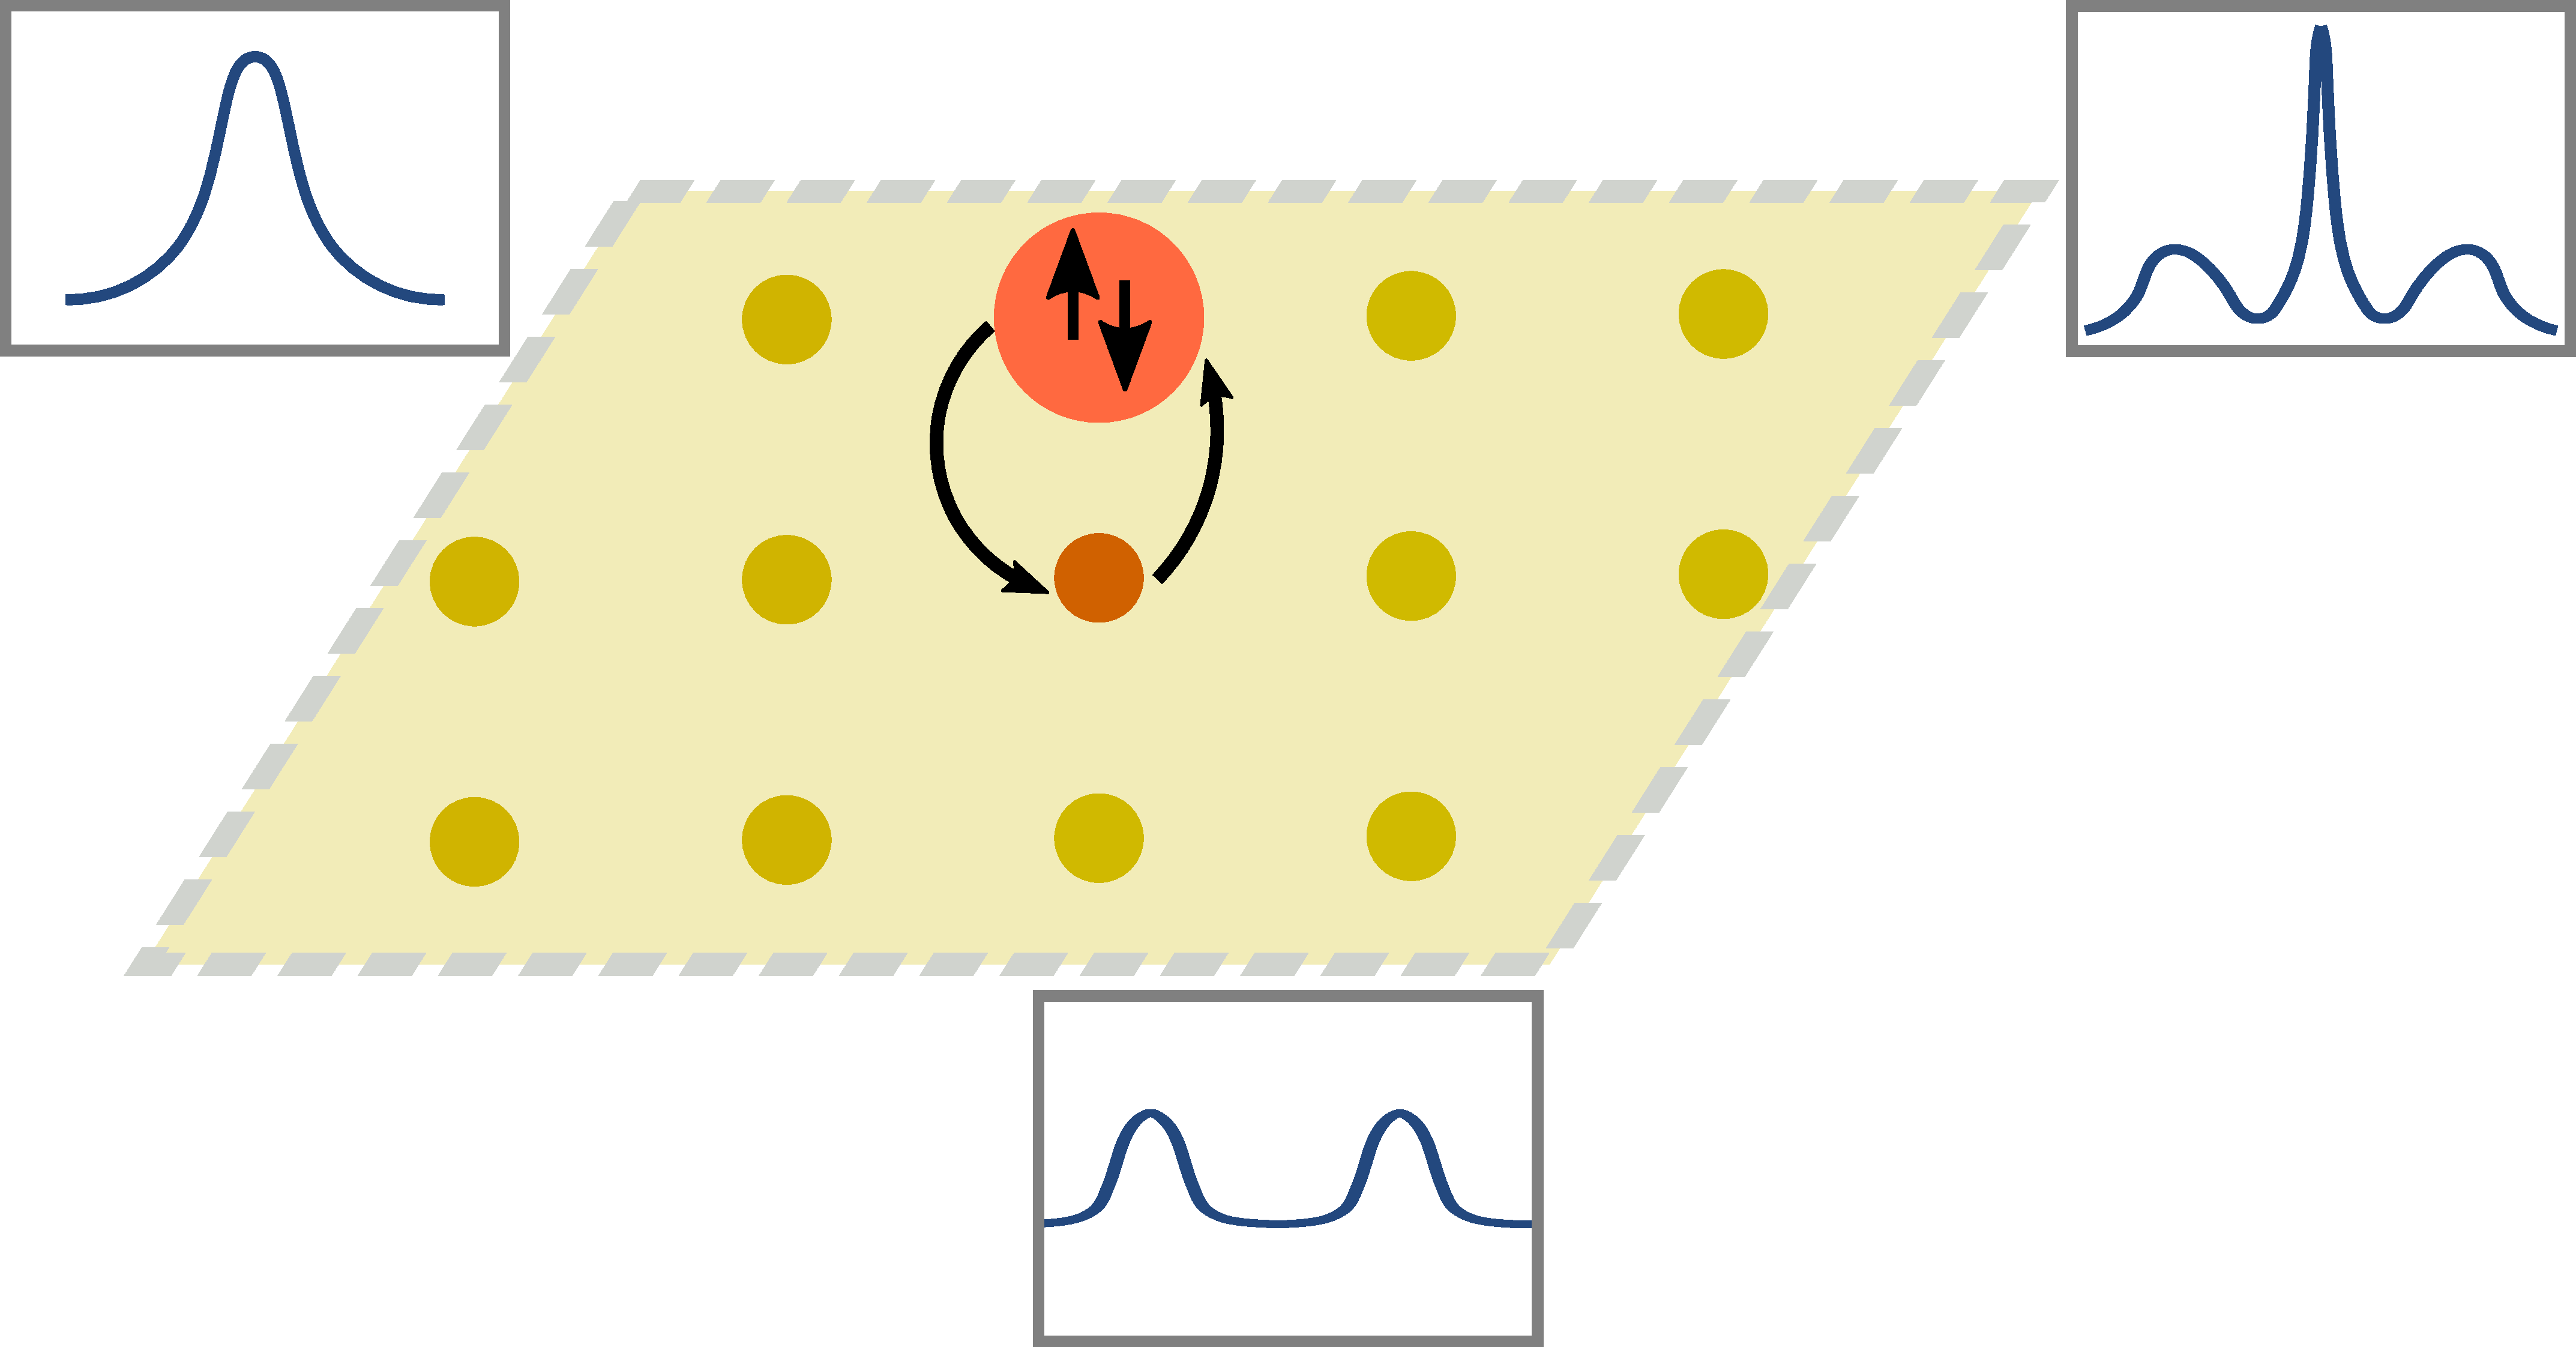
\includegraphics[width=0.8\textwidth]{DMFT.pdf}
\end{minipage}
\hspace*{\fill}
\begin{minipage}{0.45\textwidth}
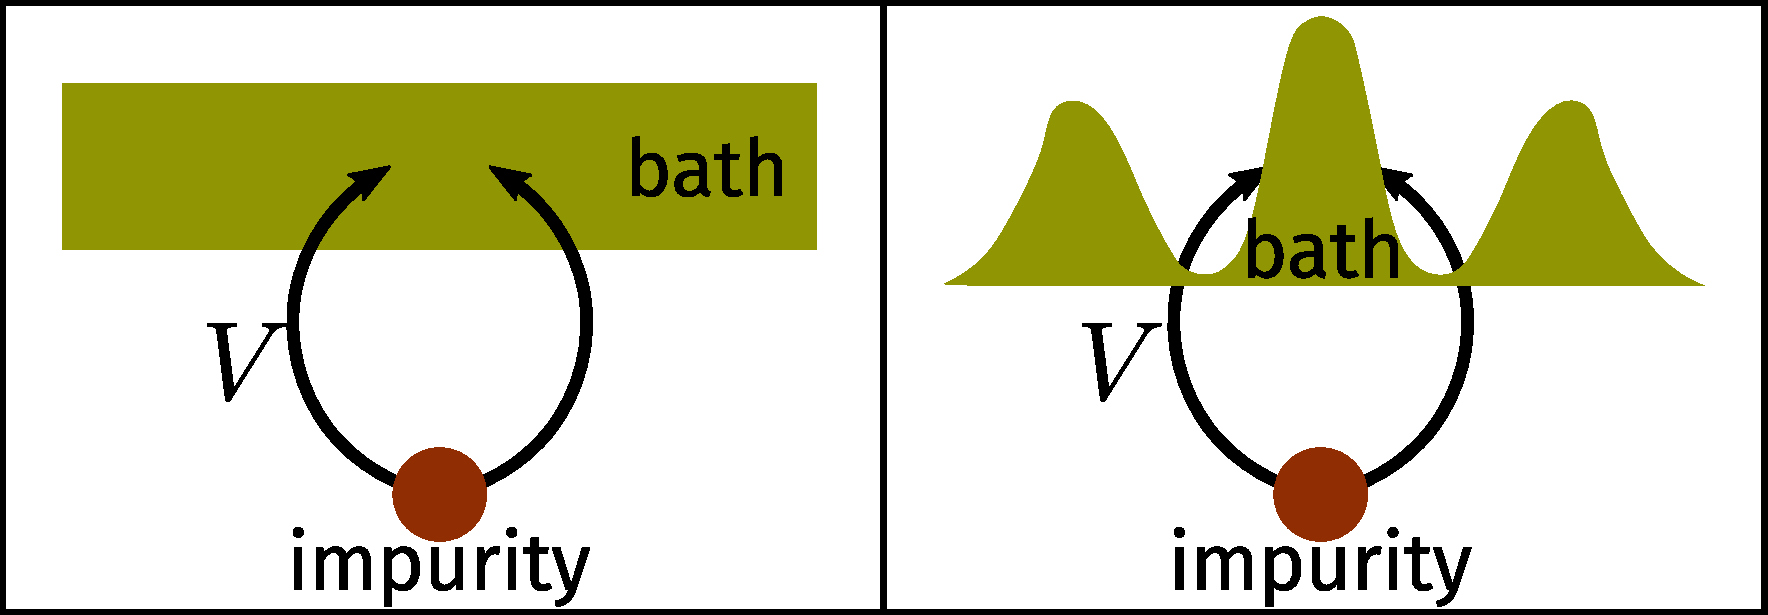
\includegraphics[width=\textwidth]{dos_diff.pdf}
\end{minipage}

\end{frame}

\begin{frame}{}
\section{Introducing the extended Anderson impurity model}
\end{frame}

\begin{frame}{DMFT on the Bethe lattice: Exact in \(d=\infty\)}
\footcite{metzner_volhardt_1989,kotliar1996,parcollet_2004,maier_2005,kotliar_rmp_2006,ohashi_2008,held_2013,sen_2020}

\begin{itemize}
\begin{minipage}{0.4\textwidth}
\nitem shows \alert{metal-insulator transition} on the Bethe lattice with \(\infty\) coordination number
\end{minipage}
\hspace*{\fill}
\begin{minipage}{0.45\textwidth}
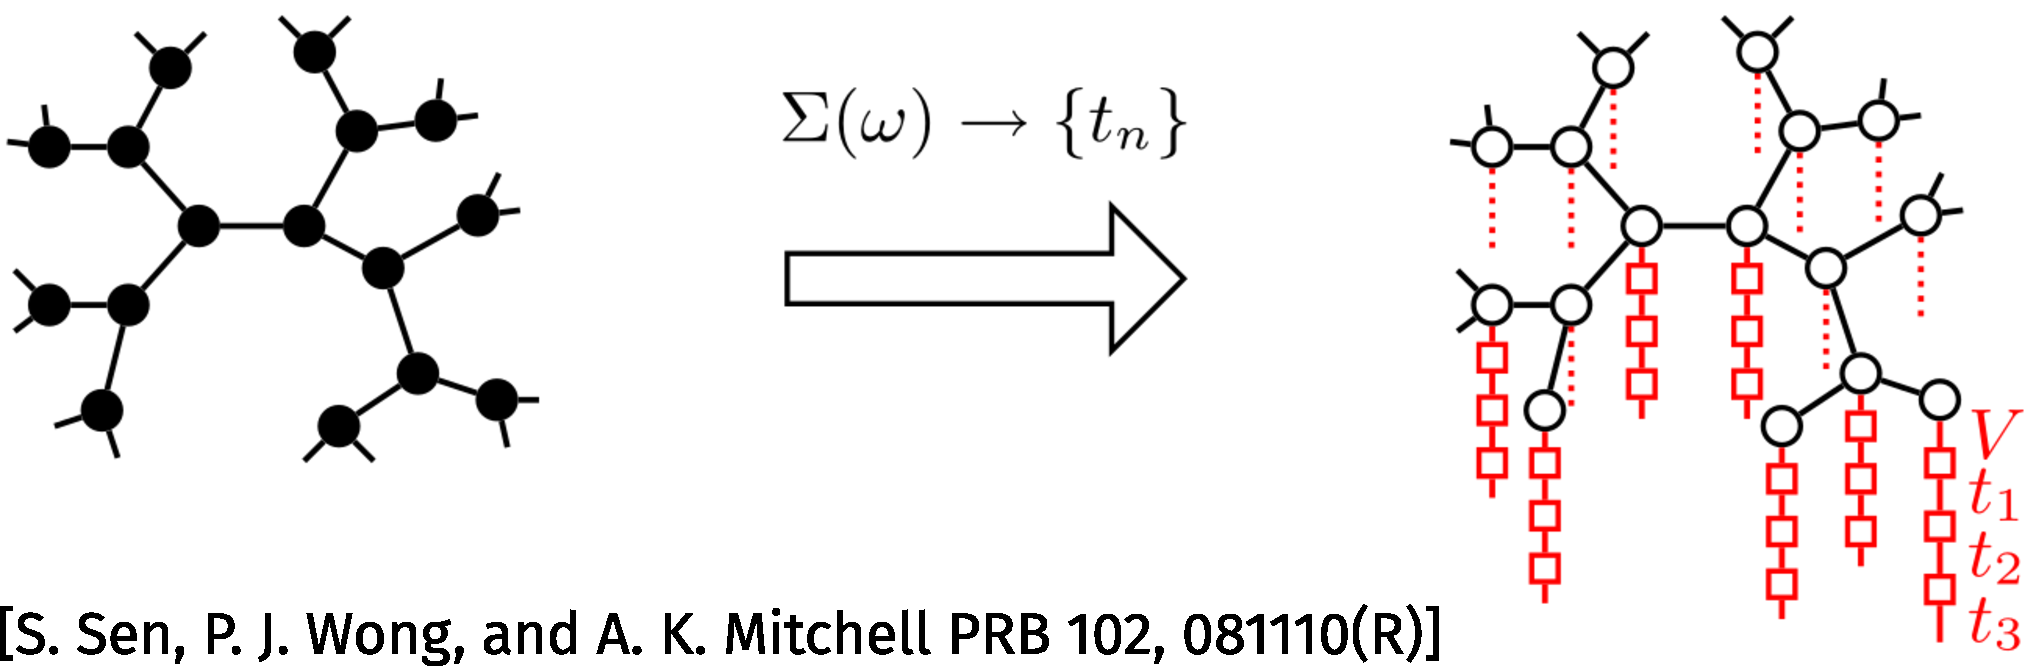
\includegraphics[width=\textwidth]{bethe-lattice.pdf}
\end{minipage}

\vspace*{\fill}

\begin{minipage}{0.45\textwidth}
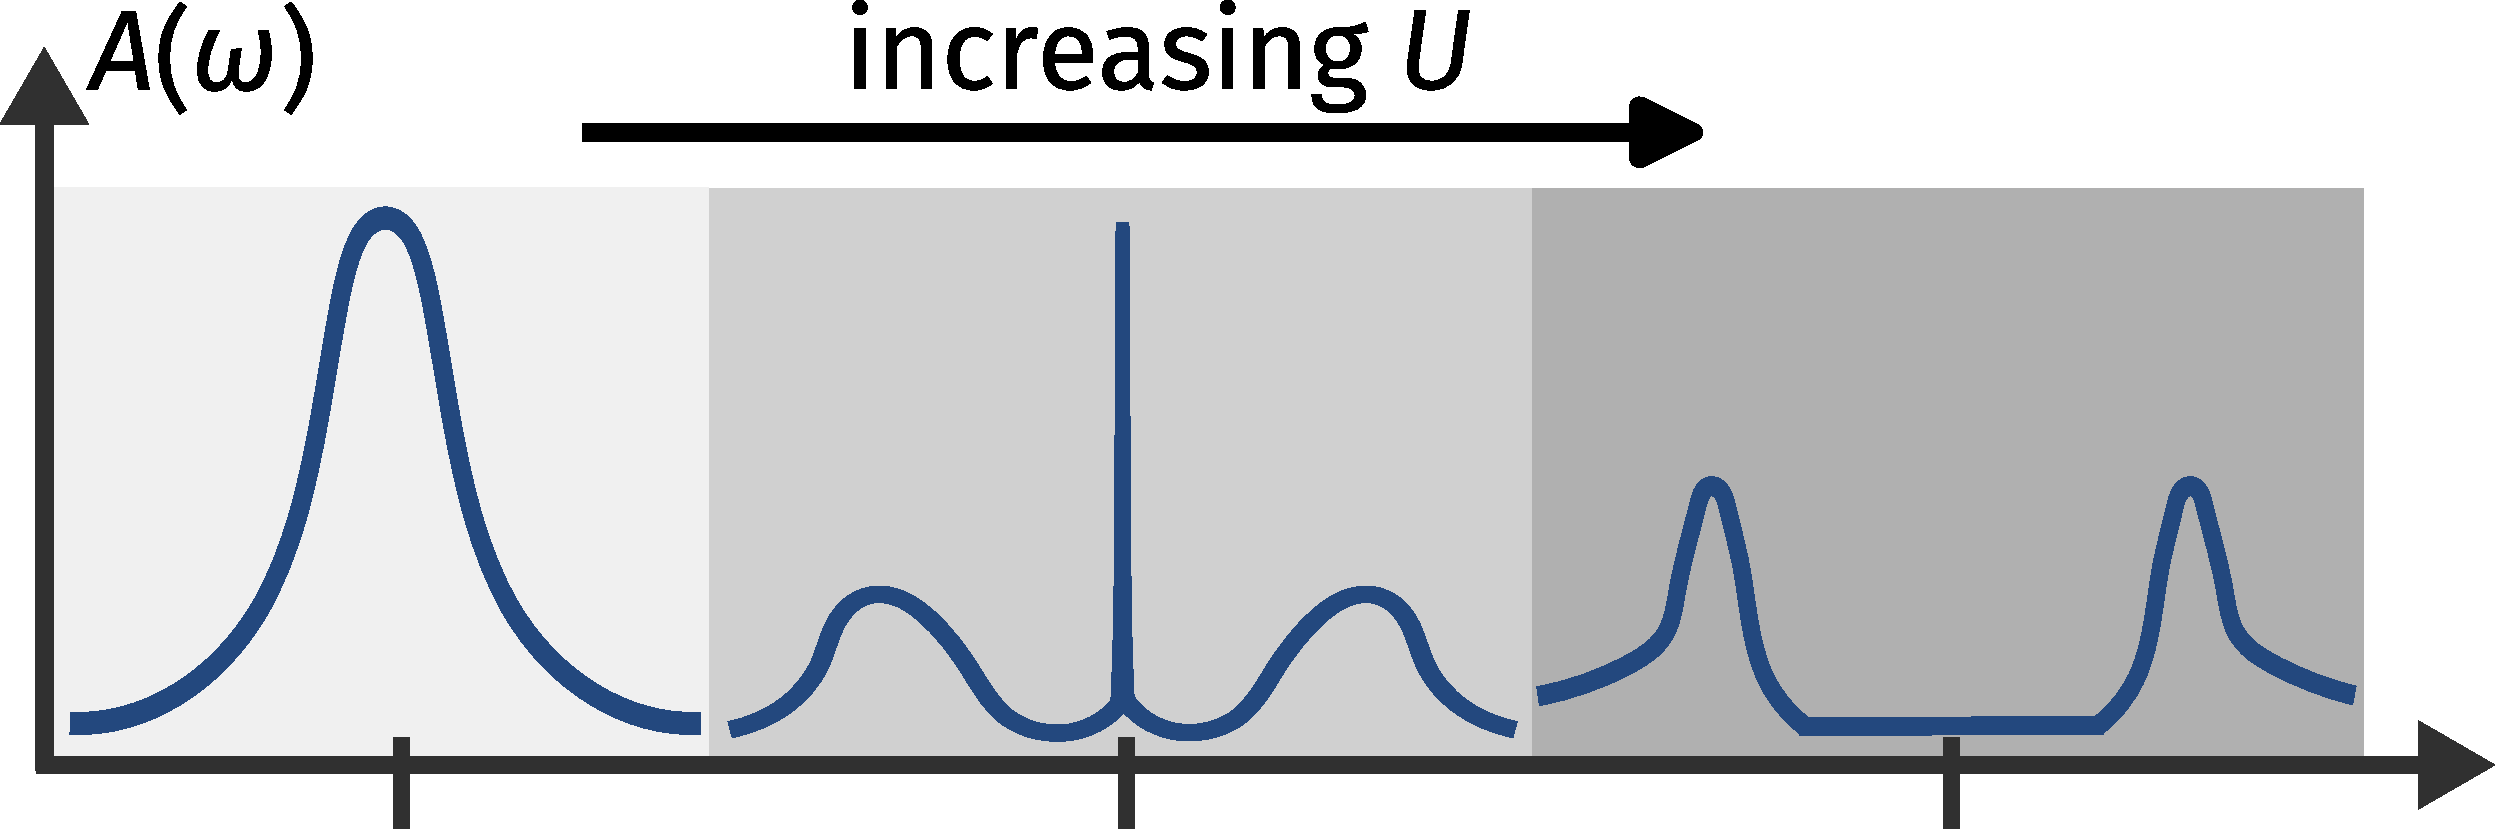
\includegraphics[width=\textwidth]{dmft-sf.pdf}
\end{minipage}
\hspace*{\fill}
\begin{minipage}{0.4\textwidth}
\nitem Spectral function develops three peaks and then \alert{gaps out}
\end{minipage}

\vspace*{\fill}

\begin{minipage}{0.4\textwidth}
\nitem Conduction bath obtained by imposing self-consistency shows \alert{non-trivial correlations}
\end{minipage}
\hspace*{\fill}
\begin{minipage}{0.45\textwidth}
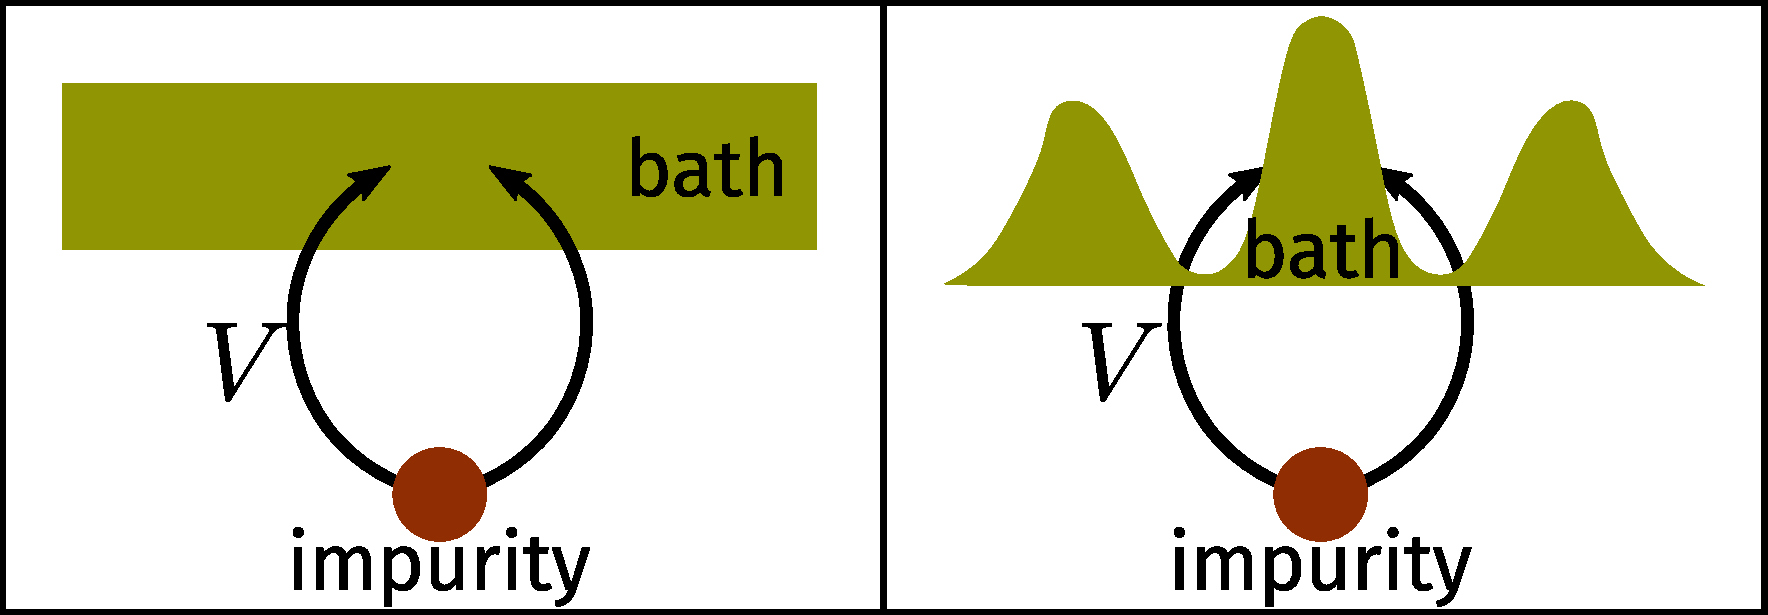
\includegraphics[width=\textwidth]{dos_diff.pdf}
\end{minipage}
\end{itemize}
	
\end{frame}

\begin{frame}{DMFT on the Bethe lattice: Exact in \(d=\infty\)}
\centering
\hspace*{-20pt}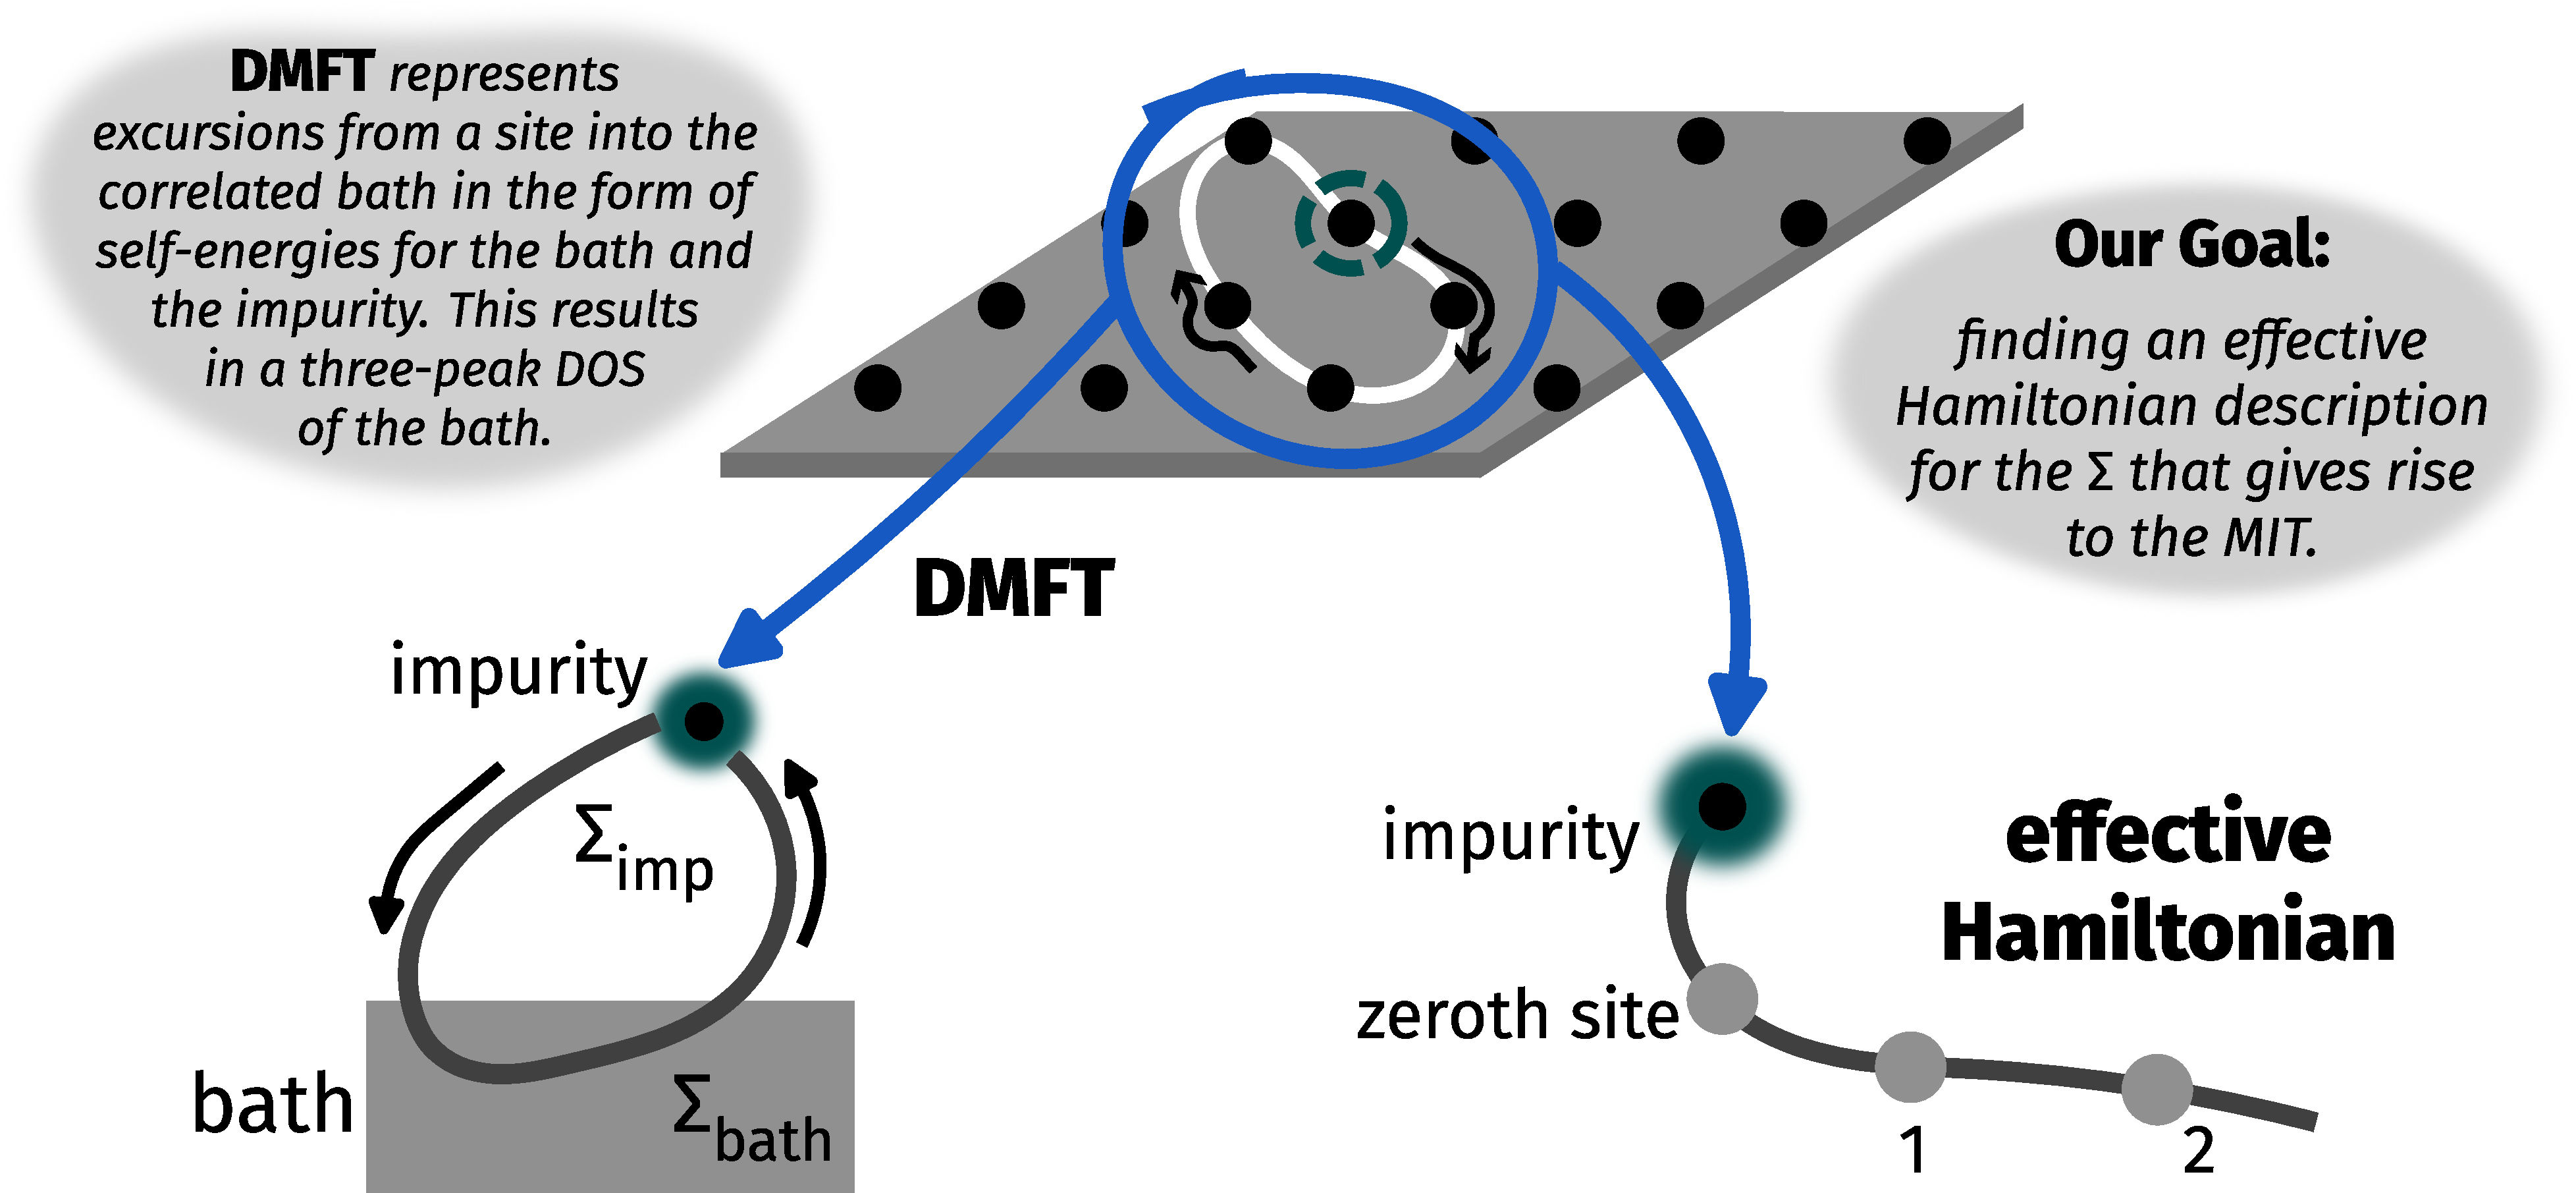
\includegraphics[width=1.1\textwidth]{contrast2.pdf}
\end{frame}

\begin{frame}{DMFT on the Bethe lattice: Exact in \(d=\infty\)}
\centering
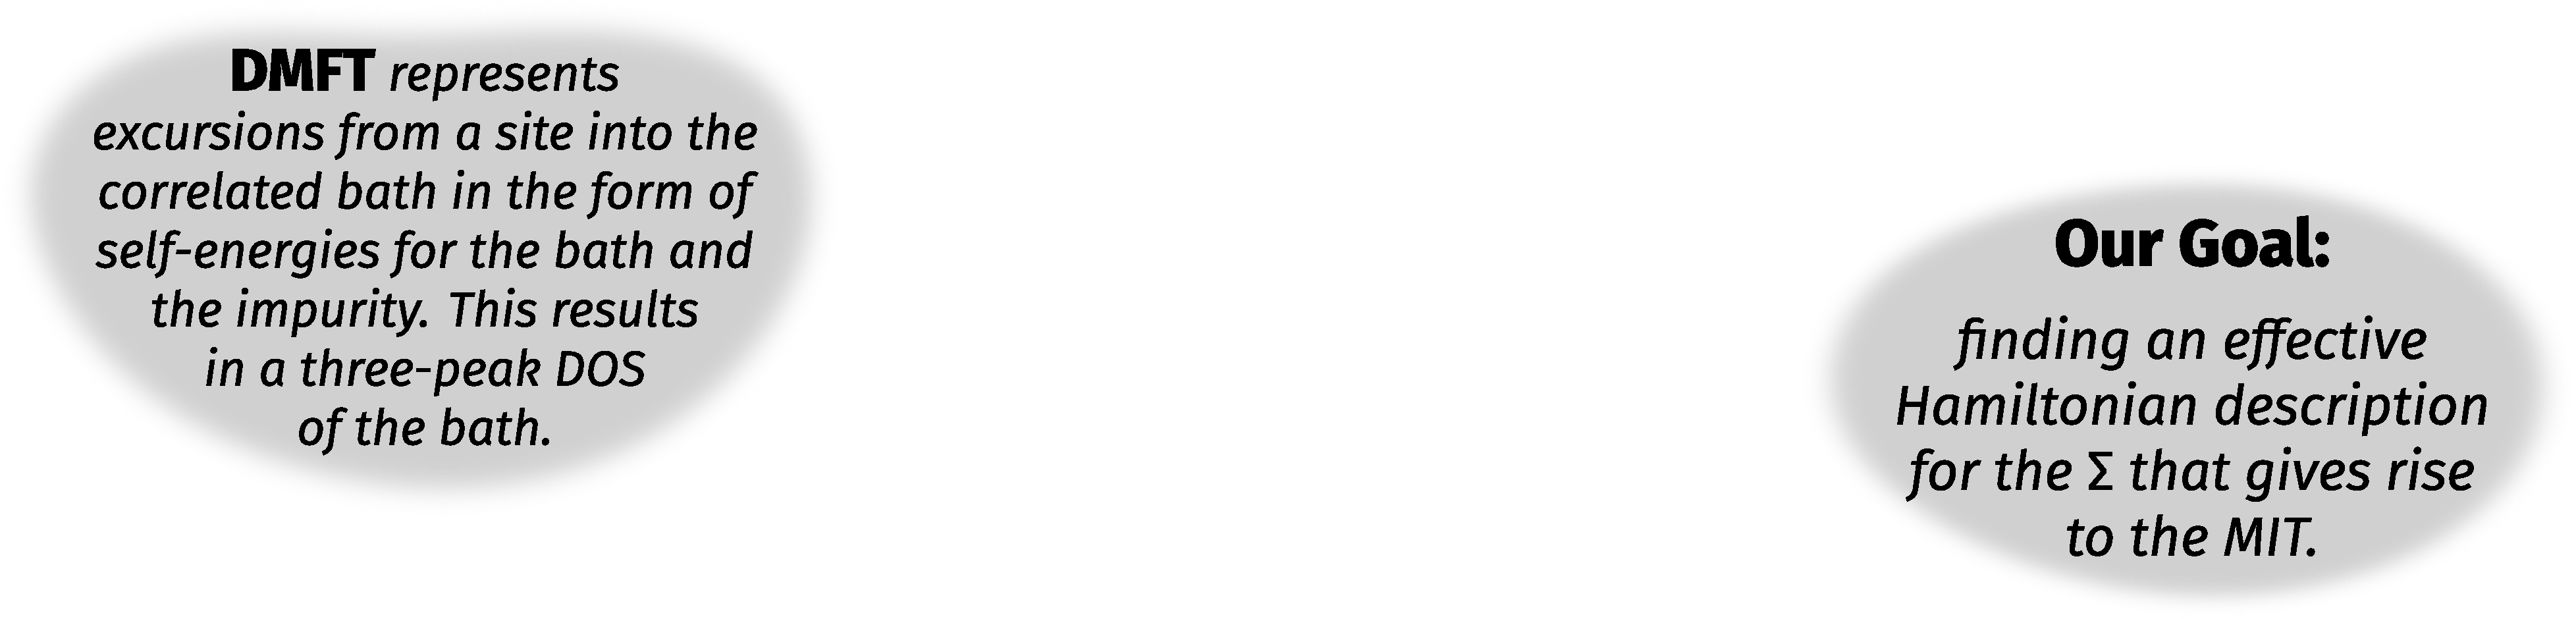
\includegraphics[width=\textwidth]{contrast3.pdf}

\vspace*{\fill}

Similar approach was adopted by Si \& Kotliar for an extended Hubbard model~\footcite{si_kotliar_1993,Kotliar_1993}.
\end{frame}

\begin{frame}{Introducing the extended Anderson impurity model}
\footcite{anderson_1961,anderson_1978,wilson1974,nozieres1974fermi,hrk_wilson_1980,andrei_1980,tsvelickKondoreview,hewson1993,costi_hewson_1990,costi2000,kuramoto1987,Cox1988}

\begin{minipage}{0.5\textwidth}
{\bf Standard Anderson impurity model\\}
\begin{itemize}
	\nitem no local-moment phase, \(A(\omega)\) gapless
	\nitem cannot explain insulating phase of DMFT
\end{itemize}
\end{minipage}
\hspace*{\fill}
\begin{minipage}{0.45\textwidth}
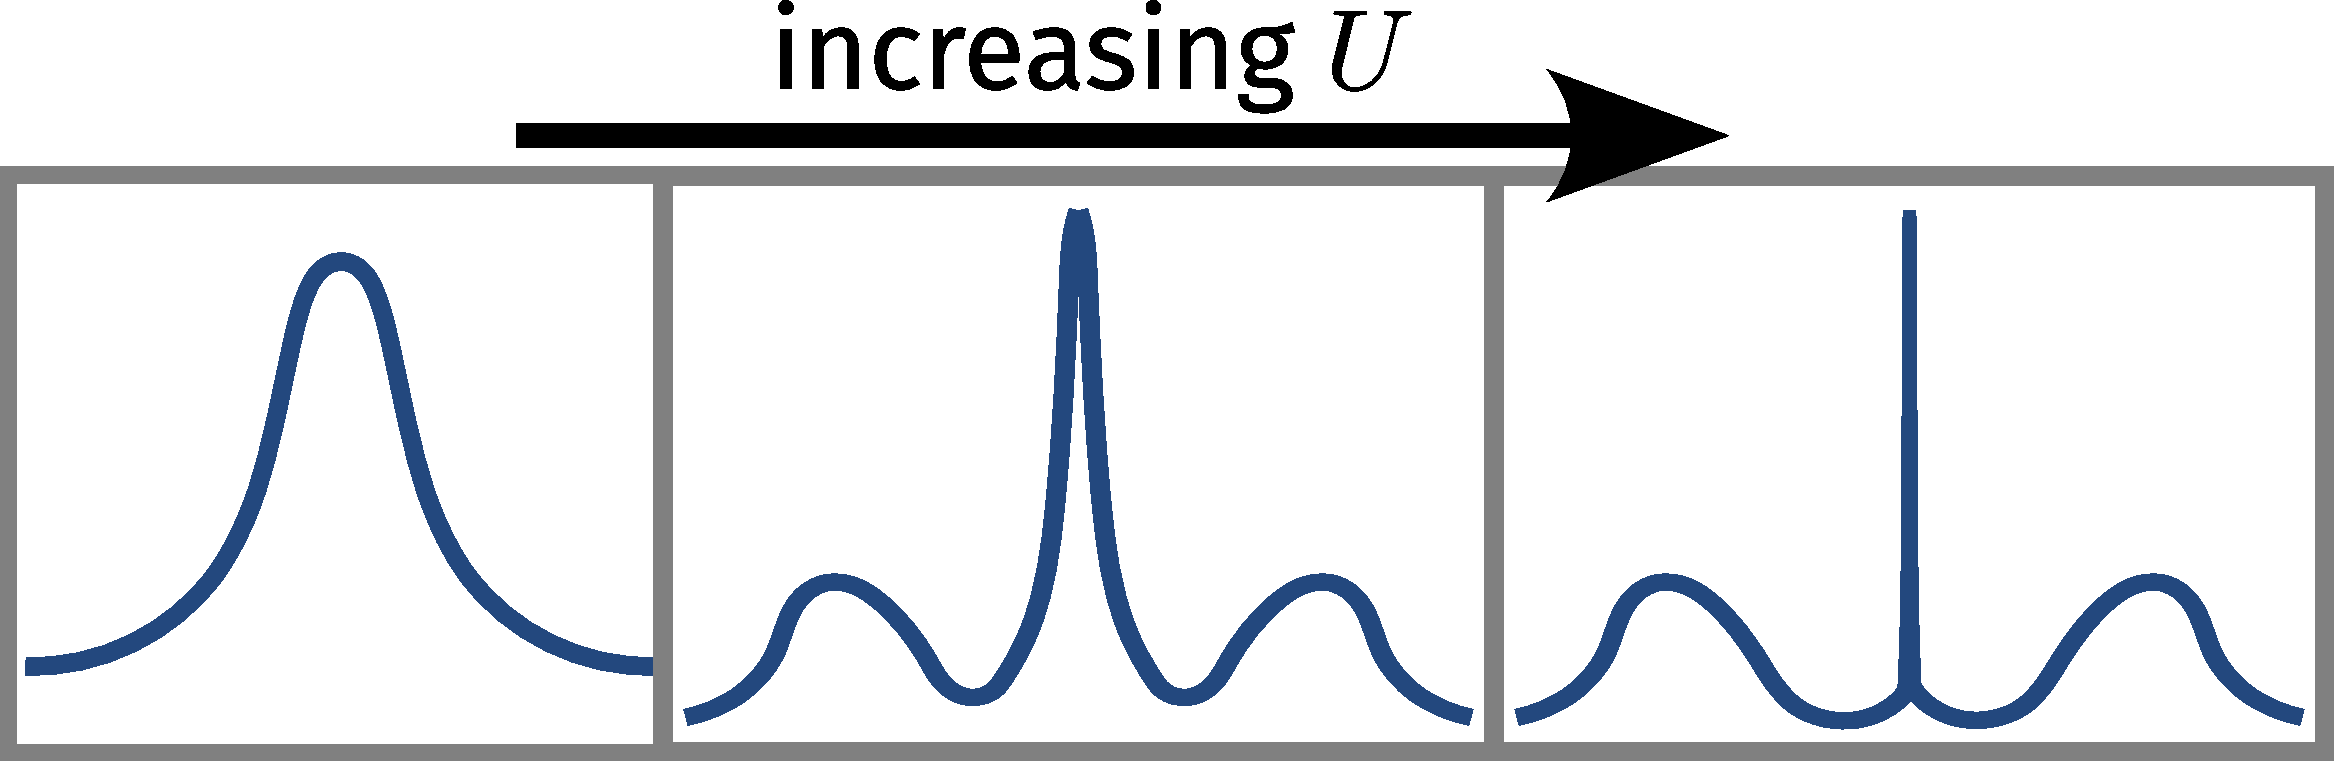
\includegraphics[width=\textwidth]{standard-siam.pdf}
\end{minipage}

\vspace*{20pt}

\alert{Gap in spectral function requires additional physics!}

\vspace*{20pt}

\begin{minipage}{0.5\textwidth}
\textbf{{\it Extended} Anderson impurity model\\}
\begin{itemize}
\nitem impurity-bath spin correlation: \(J\)
\nitem bath zeroth site local correlation: \(U_b\)
\end{itemize}
\end{minipage}
\hspace*{\fill}
\begin{minipage}{0.48\textwidth}
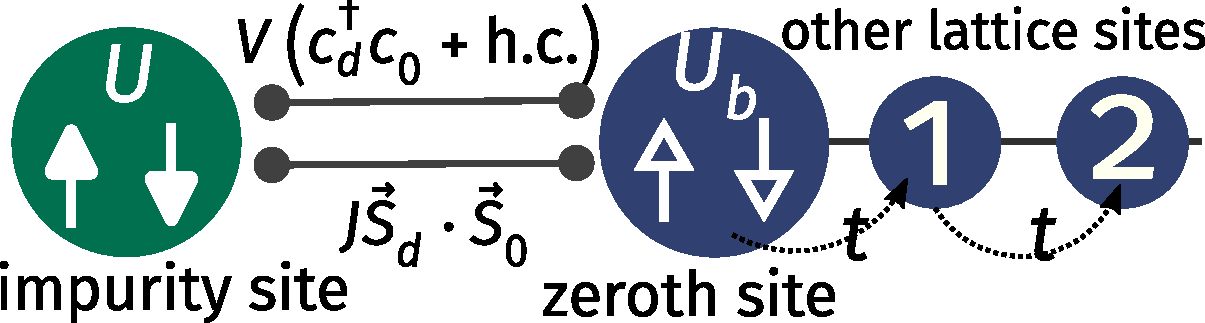
\includegraphics[width=\textwidth]{zeromode_bare.pdf}
\end{minipage}

\end{frame}

\begin{frame}{}
\section{Phase Diagram \& Ground-States}
\end{frame}

\begin{frame}{Nature of RG flows}

\begin{itemize}
	\nitem URG Equations reveal \alert{critical} point at  \(r = -U_b / J = 1/4\):
	\nitem RG equation for most dominant coupling \(J\):
	\[\Delta J = J(J + 4U_b)n(D)\frac{1}{\omega - D/2 + U_b/2 + J/4}\]
\nitem allows averting strong-coupling behaviour\\[5pt]
\nitem \(U_b\) always marginal
\end{itemize}

\vspace*{\fill}

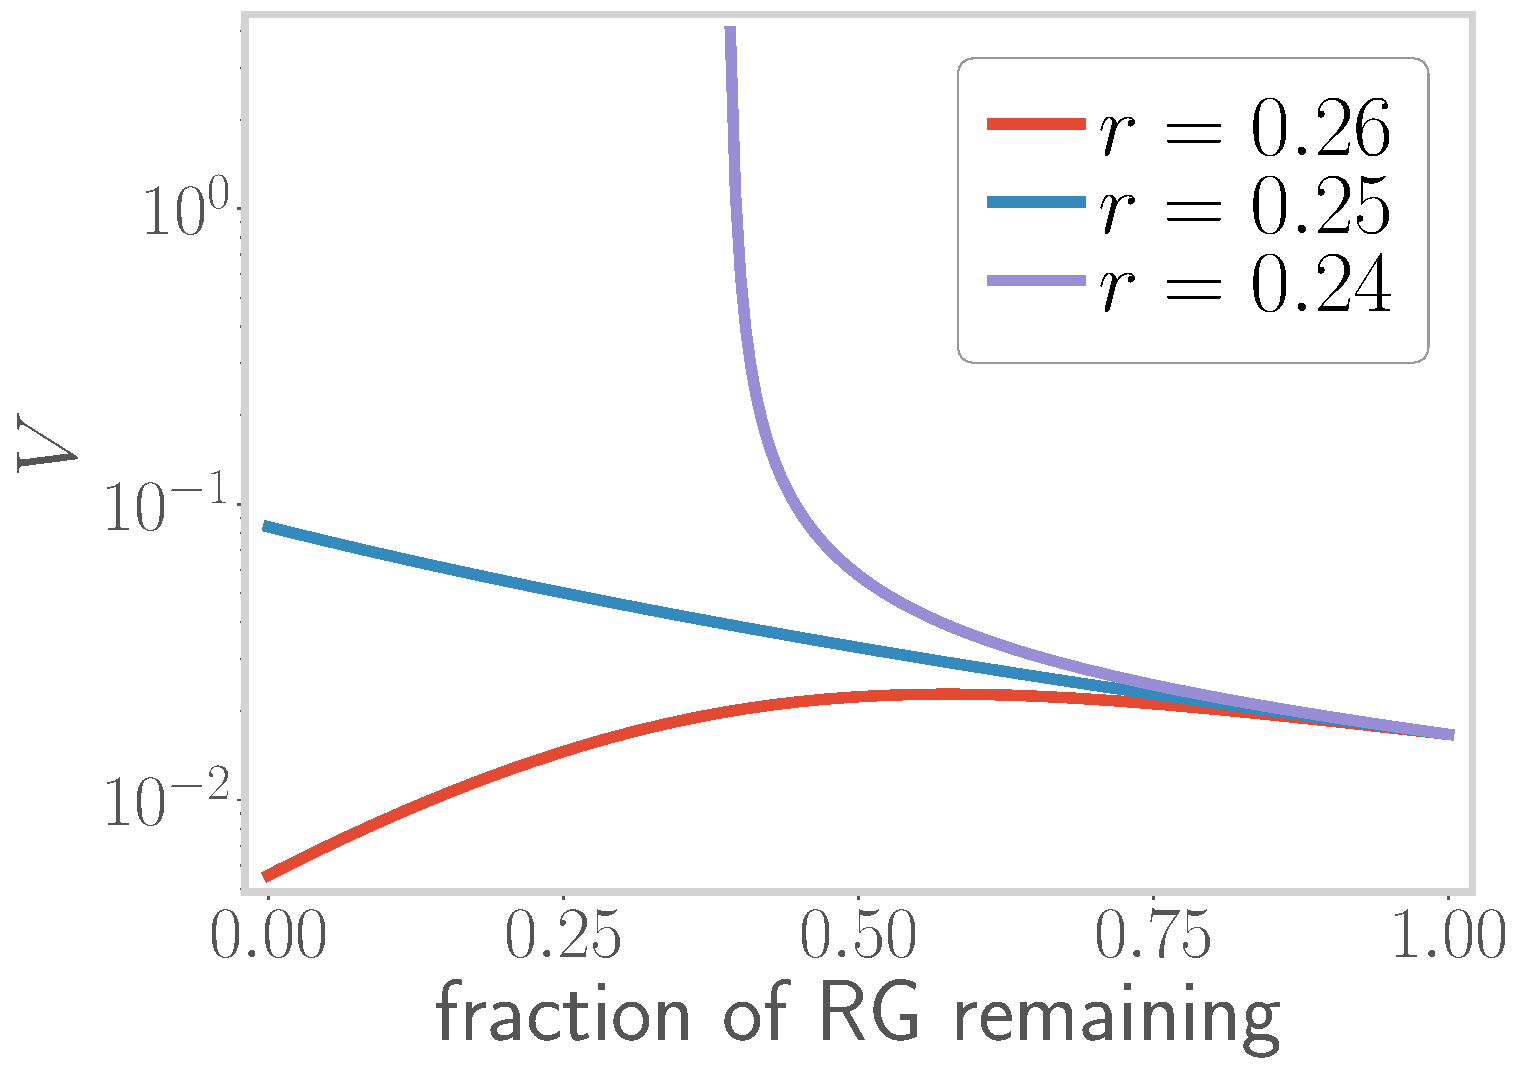
\includegraphics[width=0.45\textwidth]{V_Ub.pdf}
\hspace*{\fill}
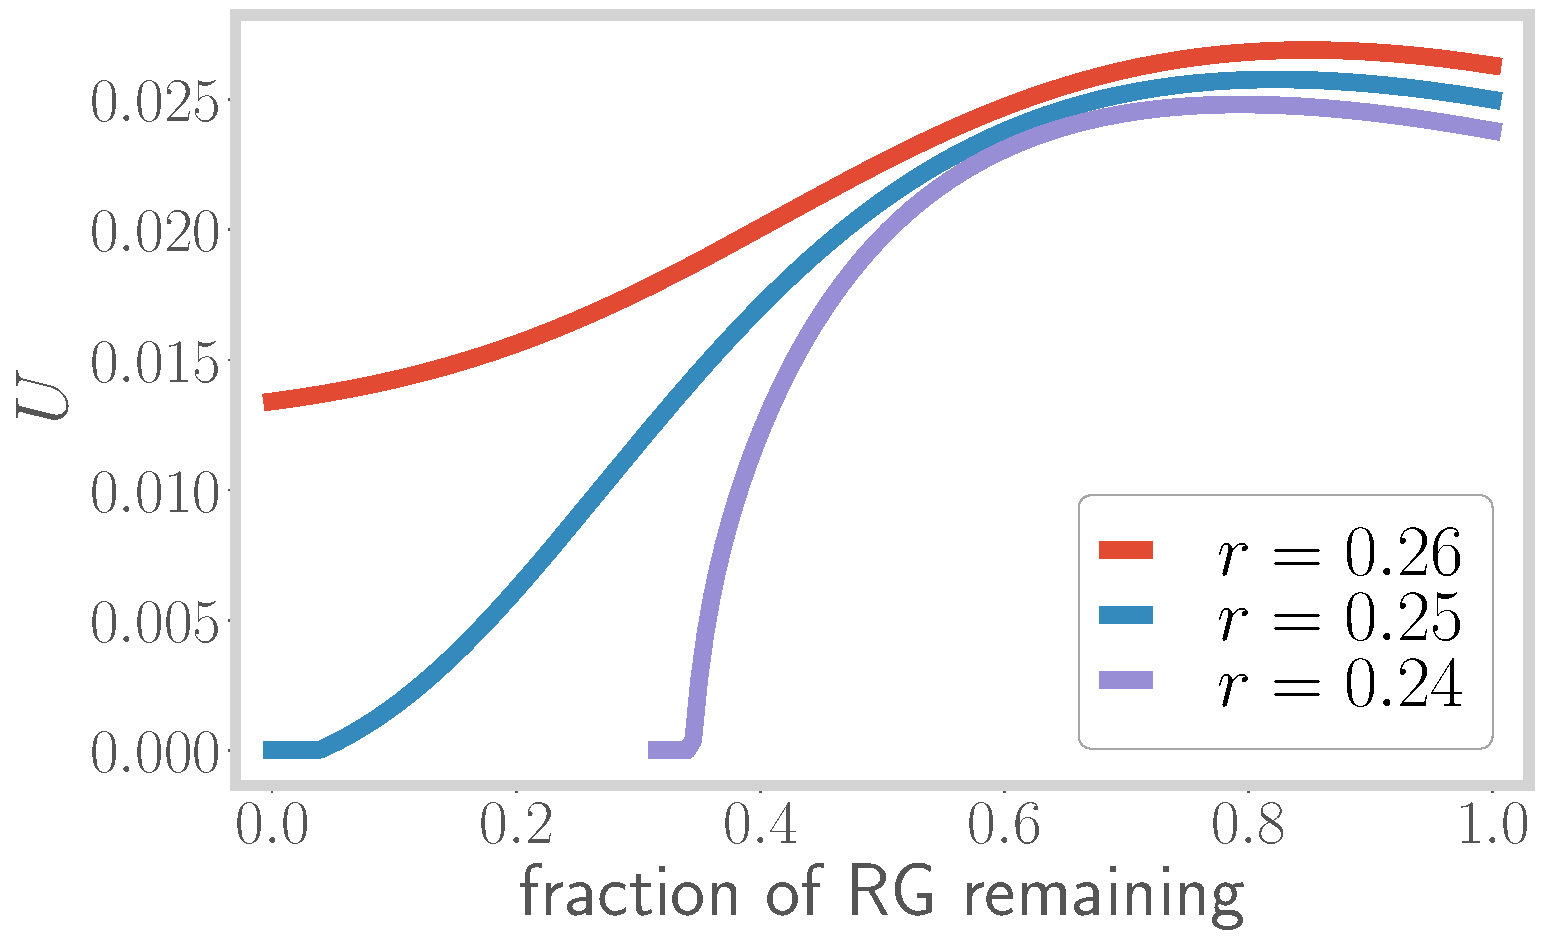
\includegraphics[width=0.45\textwidth]{U_Ub.pdf}

\end{frame}

\begin{frame}{RG Phase Diagram}
\centering

\flushright
\begin{minipage}{0.7\textwidth}
\begin{enumerate}
\nitem blue phase \(\longrightarrow\) \(U_b < -J/4\) : \(V,J\) are \alert{irrelevant} \(\longrightarrow\) local moment flows
\end{enumerate}
\end{minipage}

\vspace*{\fill}

\begin{minipage}{0.45\textwidth}
\begin{enumerate}
\nitem yellow phase: \(J \ll D_0\): involves \alert{\(V,U,U_b\)}\\[5pt]
{\it vanishes for large systems}\\
\vspace*{40pt}
\nitem gray phase: \(J \sim D_0\): \alert{all} couplings irrelevant\\[5pt]
{\it vanishes for large systems}
\end{enumerate}
\end{minipage}
\hspace*{\fill}
\begin{minipage}{0.5\textwidth}
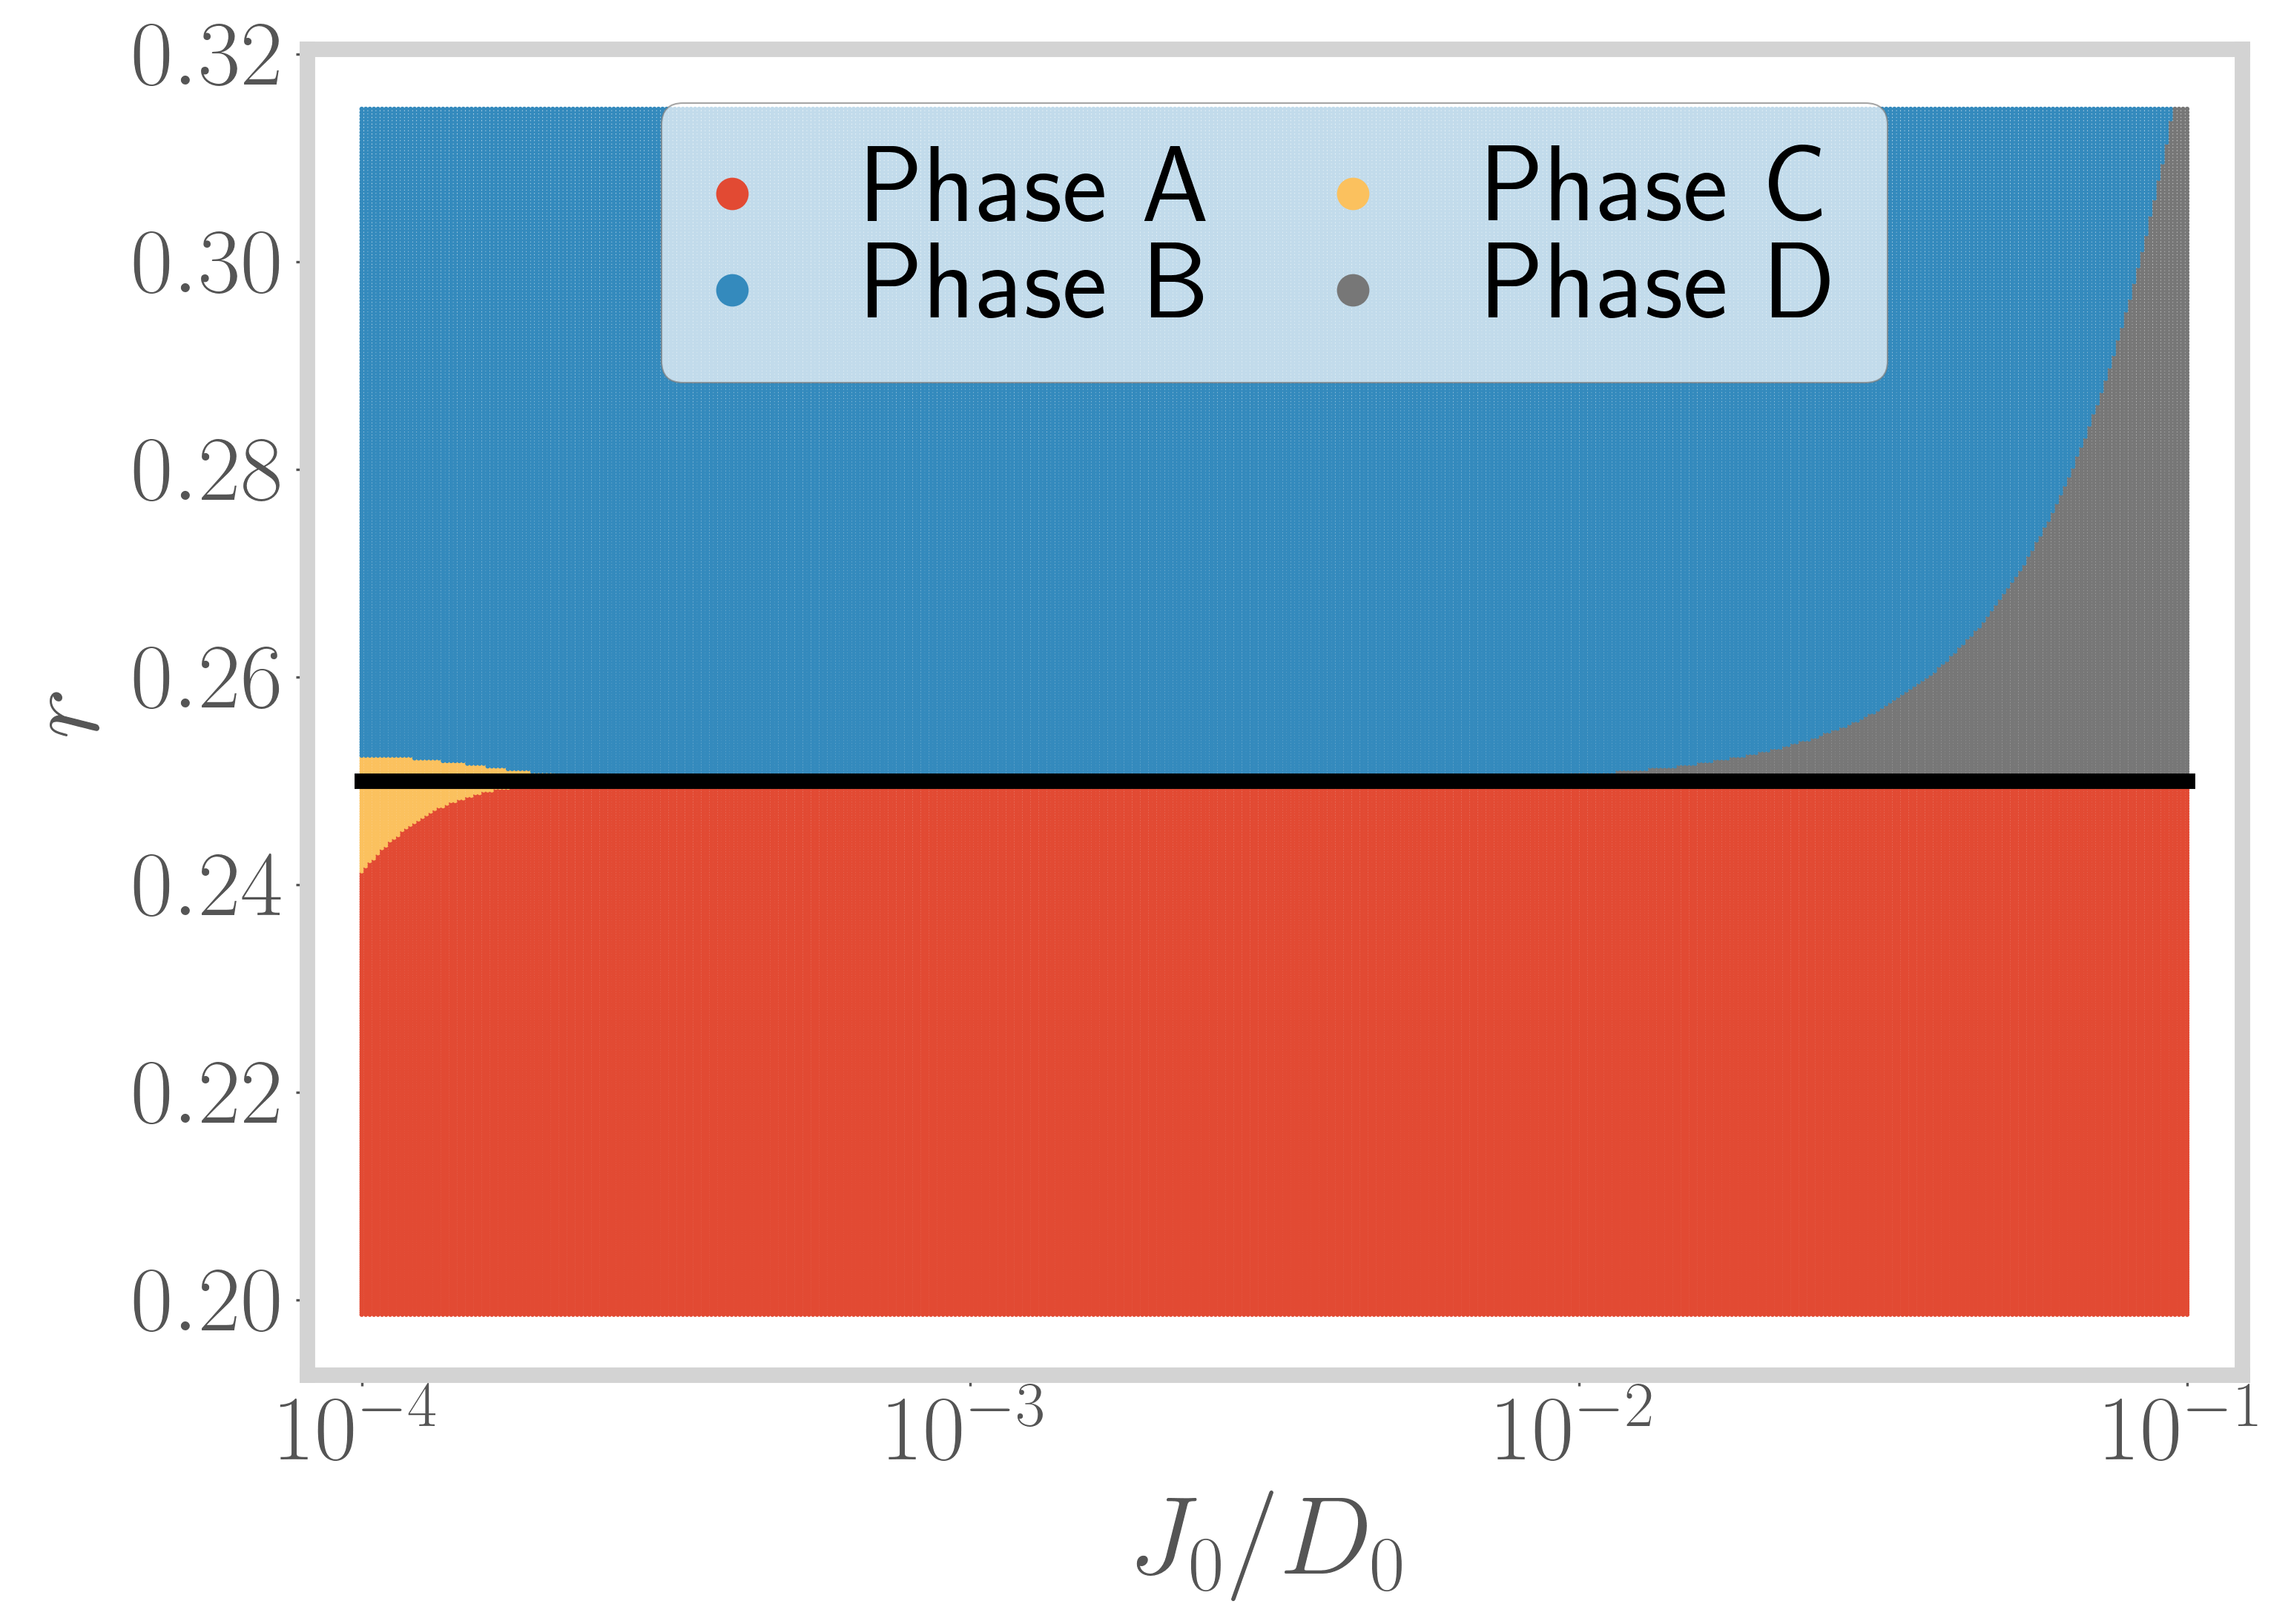
\includegraphics[width=\textwidth]{phase-map-MIT.png}
\end{minipage}

\vspace*{\fill}

\flushright
\begin{minipage}{0.7\textwidth}
\begin{enumerate}
\nitem red phase \(\longrightarrow\) \(U_b > -J/4\): \(V,J\) are \alert{relevant} \(\longrightarrow\) strong-coupling flows
\end{enumerate}
\end{minipage}

\end{frame}

\begin{frame}{Low-energy effective Hamiltonians and ground-states}

\only<1-2>{
{\Large \bf Regime 1: ~ \(|U_b| < J/4\)}

\vspace*{\fill}

\only<1>{
\begin{minipage}{0.4\textwidth}
\begin{itemize}
\nitem \(J\) relevant,\\[5pt]
\nitem \(V\) subdominant,\\[5pt]
\nitem \(U\) irrelevant\\[10pt]
\end{itemize}
\[H = J \vec{S}_d\cdot\vec{S}_0 - U_b\left( \hat n_{0 \uparrow} - \hat n_{0 \downarrow} \right)^2 + \sum_{k < \Lambda^*}\epsilon_k \hat n_{k\sigma}\]
\end{minipage}
\hspace*{\fill}
\begin{minipage}{0.3\textwidth}
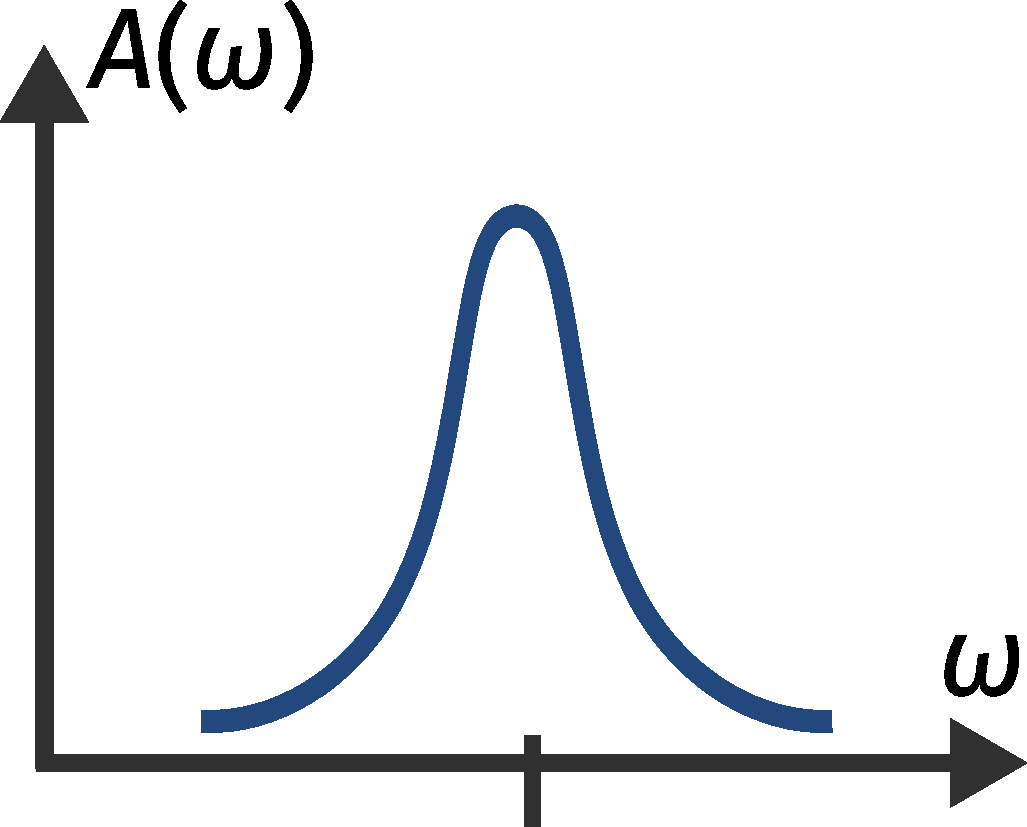
\includegraphics[width=\textwidth]{sf-1.pdf}
\end{minipage}
}
\only<2>{
{\Large \bf Zero-bandwidth limit}

\begin{minipage}{0.4\textwidth}
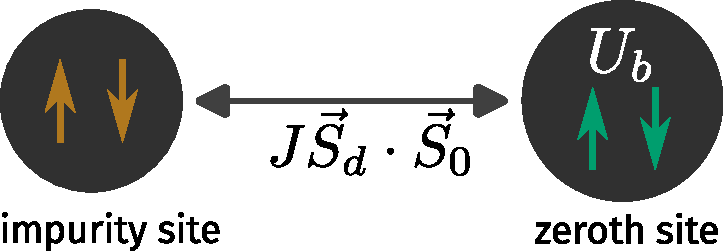
\includegraphics[width=\textwidth]{singlet.pdf}
\[H = J \vec{S}_d\cdot\vec{S}_0 - U_b\left( \hat n_{0 \uparrow} - \hat n_{0 \downarrow} \right)^2\]
\end{minipage}
\hspace*{\fill}
\begin{minipage}{0.45\textwidth}
\vspace*{\fill}
\begin{enumerate}
\nitem two-spin Heisenberg, attractive zeroth site \\[6pt]
\nitem \alert{singlet} ground state\\[10pt]
\end{enumerate}
\[\ket{\Psi}_\text{GS} = \frac{1}{\sqrt 2}\left[\ket{\uparrow_d \downarrow_0} - \ket{\downarrow_d \uparrow_0}\right] \]
\end{minipage}
}

\vspace*{\fill}

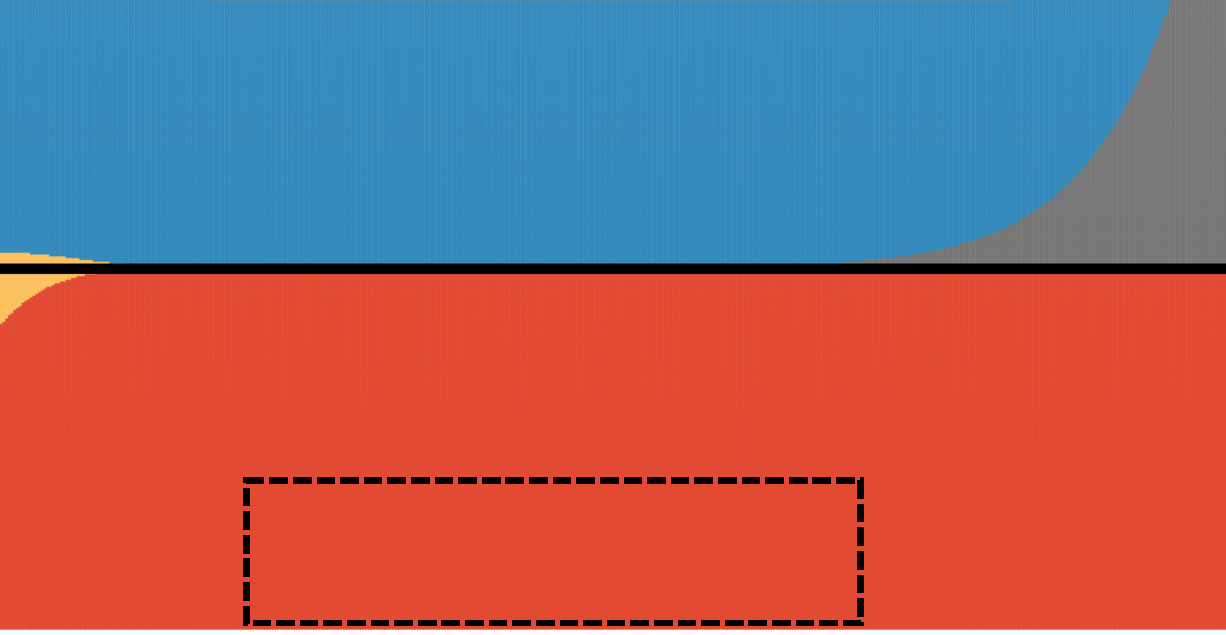
\includegraphics[width=0.45\textwidth]{phase-map-MIT1.pdf}
}

\only<3-4>{
{\Large \bf Regime 2: ~ \(|U_b| \sim J/4\)}

\vspace*{\fill}

\only<3>{
\begin{minipage}{0.4\textwidth}
\begin{itemize}
\nitem \(J\) relevant,\\[5pt]
\nitem \(V\) relevant,\\[5pt]
\nitem \(U\) irrelevant\\[10pt]
\end{itemize}
\[H = J \vec{S}_d\cdot\vec{S}_0 + V \sum_\sigma \left( c^\dagger_{d\sigma}c_{0\sigma} + \text{h.c.} \right) - U_b\left( \hat n_{0 \uparrow} - \hat n_{0 \downarrow} \right)^2 + \sum_{k < \Lambda^*}\epsilon_k \hat n_{k\sigma}\]
\end{minipage}
\hspace*{\fill}
\begin{minipage}{0.3\textwidth}
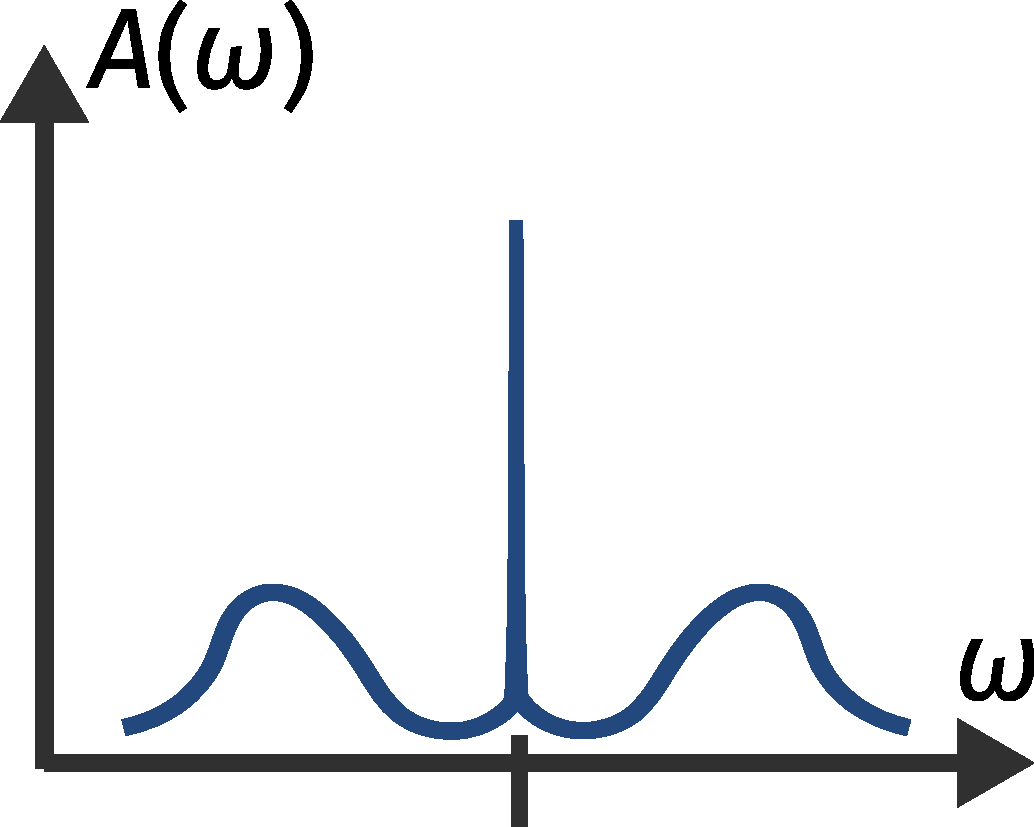
\includegraphics[width=\textwidth]{sf-3.pdf}
\end{minipage}

}
\only<4>{
{\Large \bf Zero-bandwidth limit}

\begin{minipage}{0.4\textwidth}
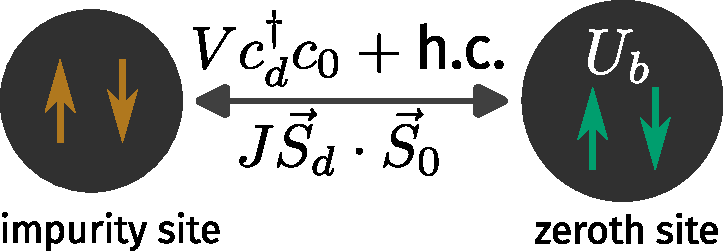
\includegraphics[width=\textwidth]{siam-JV.pdf}
\[H = J \vec{S}_d\cdot\vec{S}_0 + V \sum_\sigma \left( c^\dagger_{d\sigma}c_{0\sigma} + \text{h.c.} \right) - U_b\left( \hat n_{0 \uparrow} - \hat n_{0 \downarrow} \right)^2\]
\end{minipage}
\hspace*{\fill}
\begin{minipage}{0.45\textwidth}
\vspace*{\fill}
\begin{enumerate}
\nitem \alert{spin+charge} dimer with attractive zeroth site\\[6pt]
\nitem spin-singlet + charge-triplet-zero in gr-state\\[10pt]
\end{enumerate}
\[\ket{\Psi}_\text{GS} = \frac{1}{2\sqrt 2}\left[\ket{\uparrow_d \downarrow_0} - \ket{\downarrow_d \uparrow_0}\right] ~ + ~ \frac{1}{2\sqrt 2}\left[\ket{2_d, 0_0} - \ket{0_d, 2_0} \right] \]
\end{minipage}
}

\vspace*{\fill}

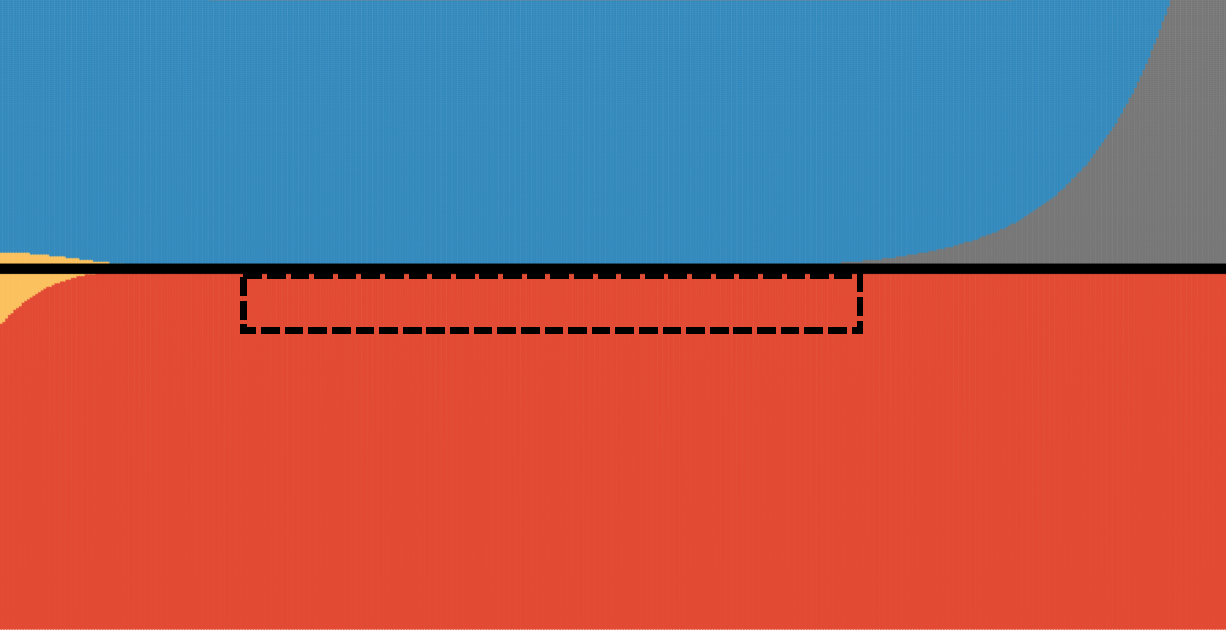
\includegraphics[width=0.45\textwidth]{phase-map-MIT2.pdf}
}

\only<5-6>{
{\Large \bf Regime 3: ~ \(|U_b| > J/4\)}

\vspace*{\fill}

\only<5>{
\begin{minipage}{0.4\textwidth}
\begin{itemize}
\nitem \(J,V\) irrelevant,\\[5pt]
\nitem \(U\) relevant,\\[5pt]
\end{itemize}
\[H = - U/2\left( \hat n_{d \uparrow} - \hat n_{d \downarrow} \right)^2 - U_b\left( \hat n_{0 \uparrow} - \hat n_{0 \downarrow} \right)^2 + \sum_{k < \Lambda^*}\epsilon_k \hat n_{k\sigma}\]
\end{minipage}
\hspace*{\fill}
\begin{minipage}{0.3\textwidth}
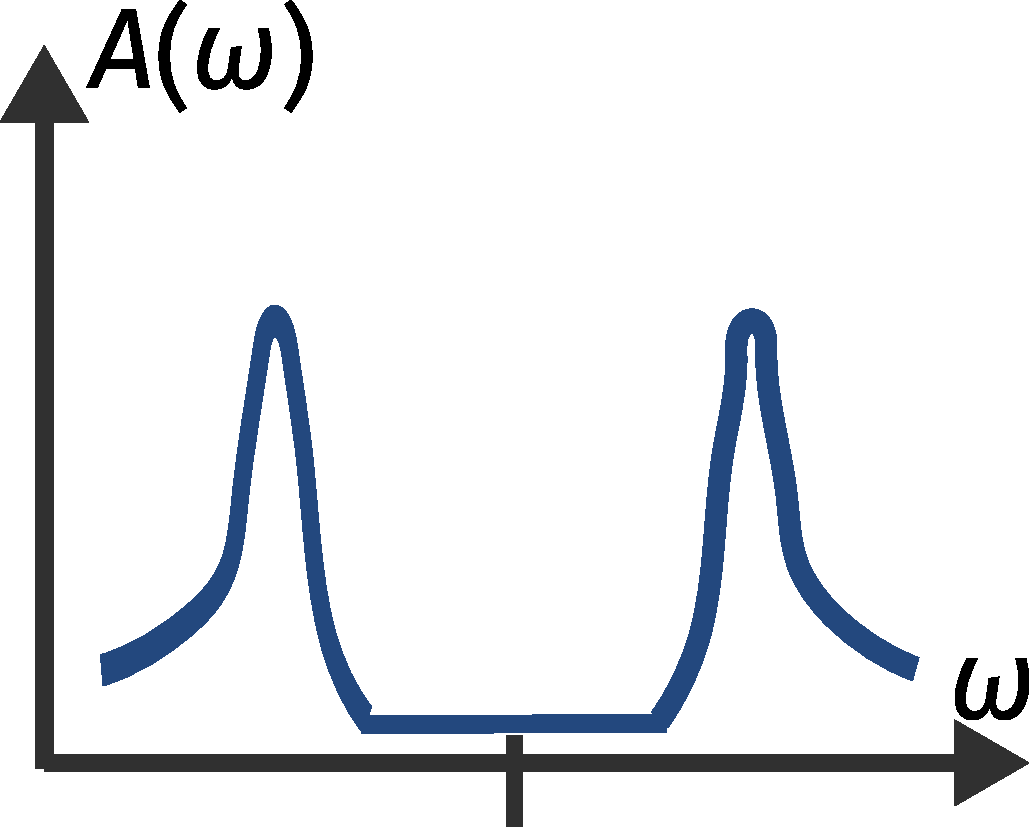
\includegraphics[width=\textwidth]{sf-4.pdf}
\end{minipage}

}
\only<6>{
{\Large \bf Zero-bandwidth limit}

\begin{minipage}{0.4\textwidth}

\includegraphics[width=\textwidth]{local-moment.pdf}
\[H = - U/2\left( \hat n_{d \uparrow} - \hat n_{d \downarrow} \right)^2 - U_b\left( \hat n_{0 \uparrow} - \hat n_{0 \downarrow} \right)^2\]
\end{minipage}
\hspace*{\fill}
\begin{minipage}{0.45\textwidth}
\vspace*{\fill}
\begin{enumerate}
\nitem impurity site detaches from bath\\[6pt]
\nitem \alert{local moment} ground-state\\[10pt]
\end{enumerate}
\[\ket{\Psi}_\text{GS} = \ket{\uparrow,\downarrow}_d\otimes\ket{0,2}_0 \]
\end{minipage}
}

\vspace*{\fill}

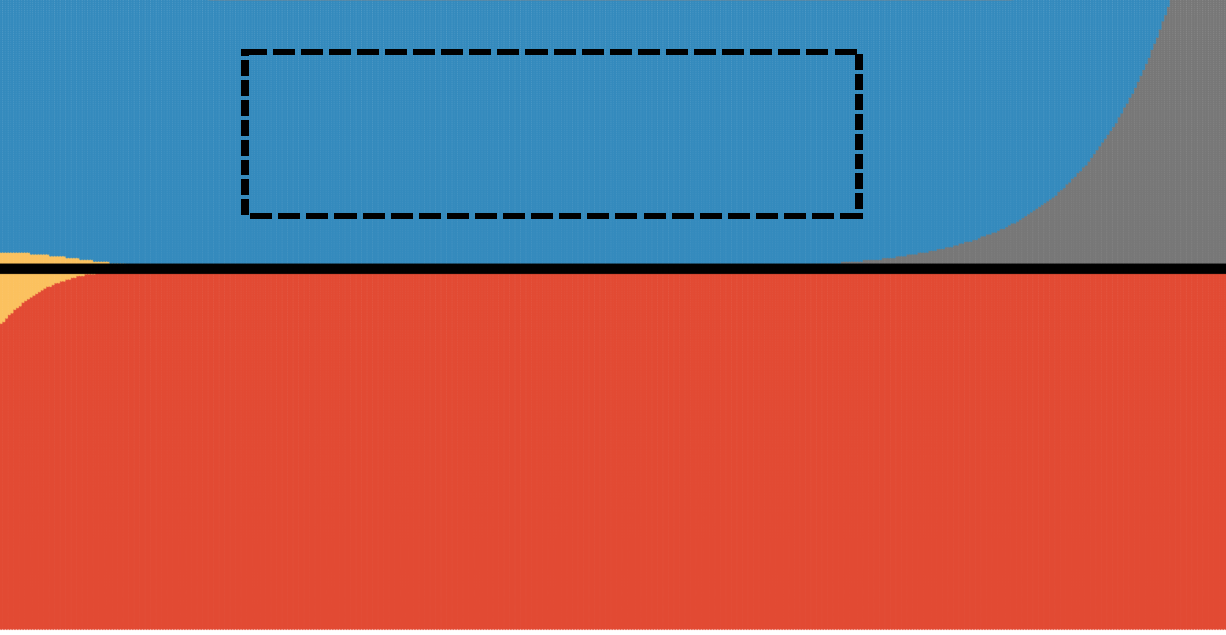
\includegraphics[width=0.45\textwidth]{phase-map-MIT3.pdf}
}

\only<7>{
\alert{Ground-state overlaps} with spin singlet and charge triplet zero\\
\vspace*{\fill}
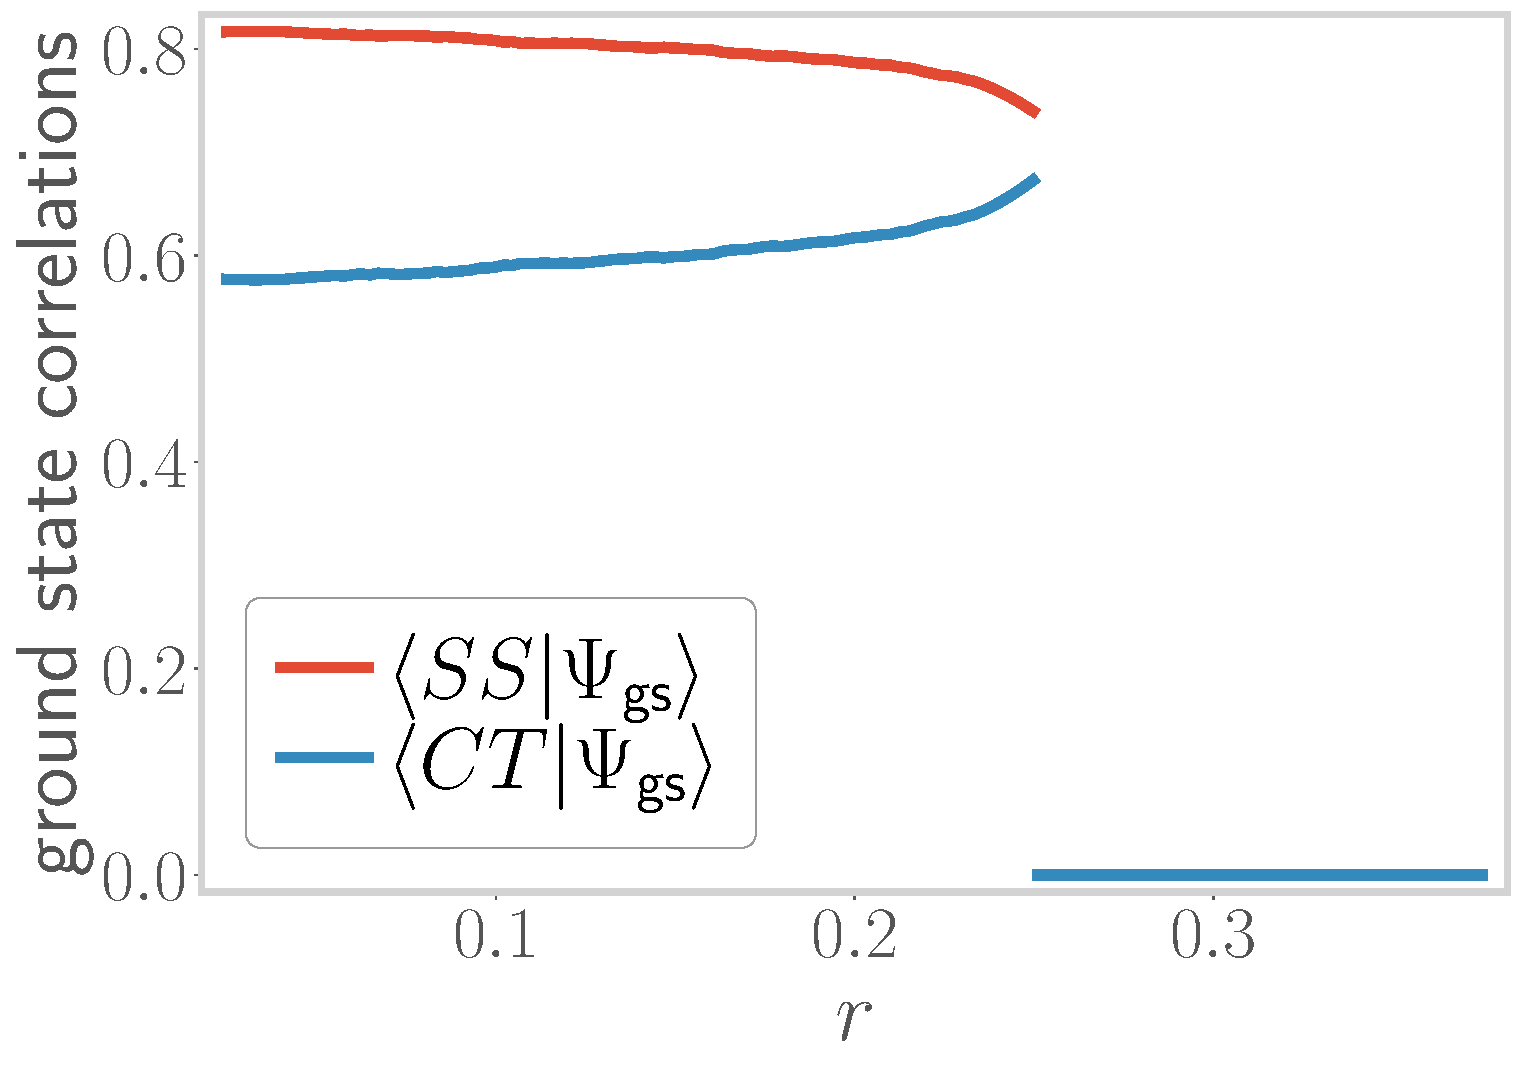
\includegraphics[width=0.6\textwidth]{corrs_gs.pdf}
}
\end{frame}

\begin{frame}{}
\section{Nature of the Transition}
\end{frame}

\begin{frame}{Gapping of the impurity spectral function}
\begin{minipage}{0.25\textwidth}
\begin{itemize}
\nitem Broad central peak at \(|U_b| \ll J/4\)
\end{itemize}
\end{minipage}
\hspace{\fill}
\begin{minipage}{0.45\textwidth}
\begin{itemize}
\nitem Correlated \alert{three peak} structure at \(|U_b| \lesssim J/4\)\\[10pt]
\end{itemize}
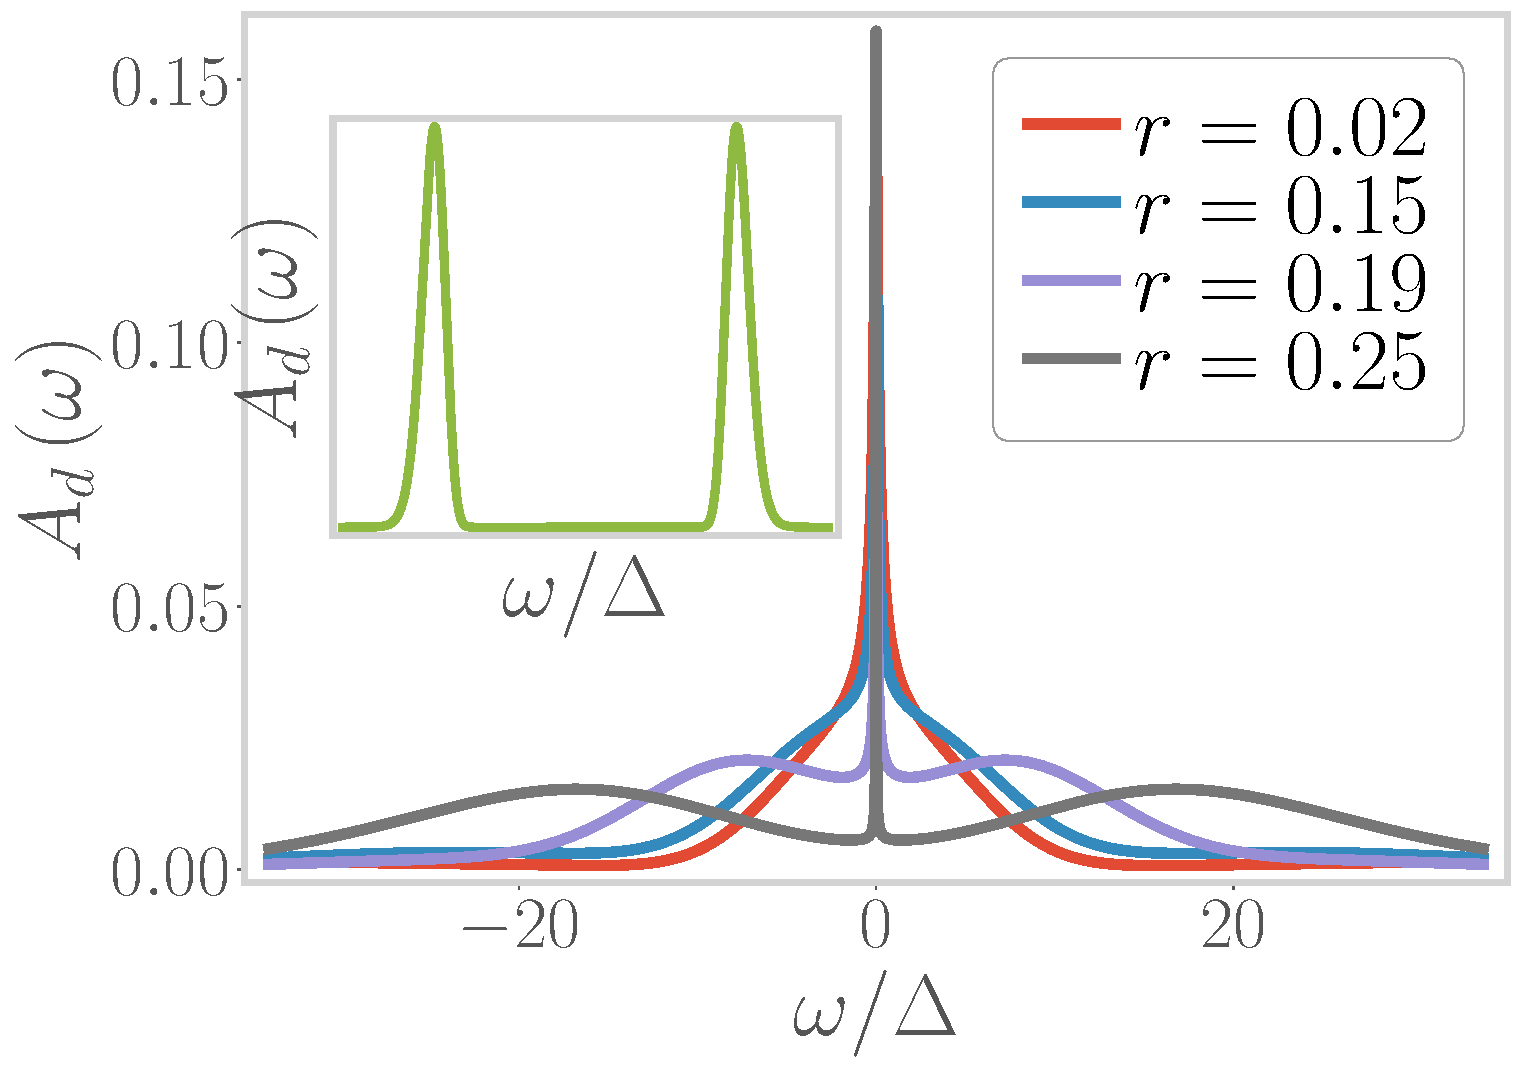
\includegraphics[width=\textwidth]{Add.pdf}
\end{minipage}
\hspace{\fill}
\begin{minipage}{0.25\textwidth}
\begin{itemize}
\nitem hard central \alert{gap} for  \(|U_b| > J/4\)
\end{itemize}
\end{minipage}

\end{frame}

\begin{frame}{Destruction of the Kondo cloud}
\centering
The Kondo cloud \alert{weakens, and is destroyed} at the transition.

\vspace*{\fill}

\begin{minipage}{0.4\textwidth}
\begin{itemize}
	\nitem vanishing of impurity-bath correlations
\end{itemize}
\end{minipage}
\hspace*{\fill}
\begin{minipage}{0.4\textwidth}
\begin{itemize}
	\nitem transfer of entanglement into the bath
\end{itemize}
\end{minipage}

\vspace*{\fill}

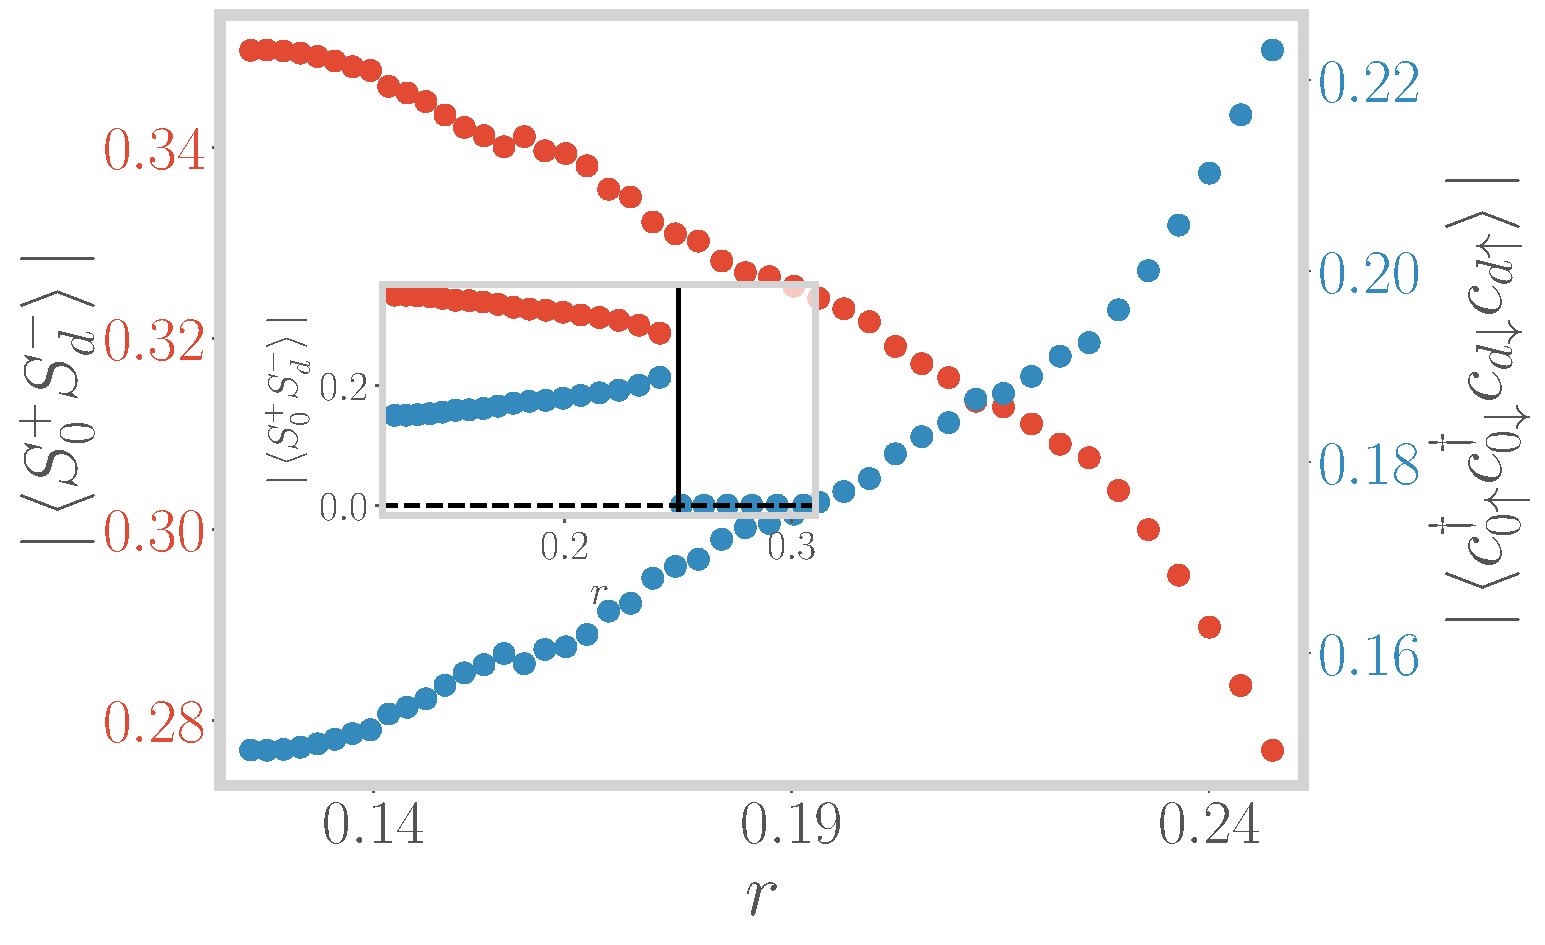
\includegraphics[width=0.45\textwidth]{pairing.pdf}
\hspace*{\fill}
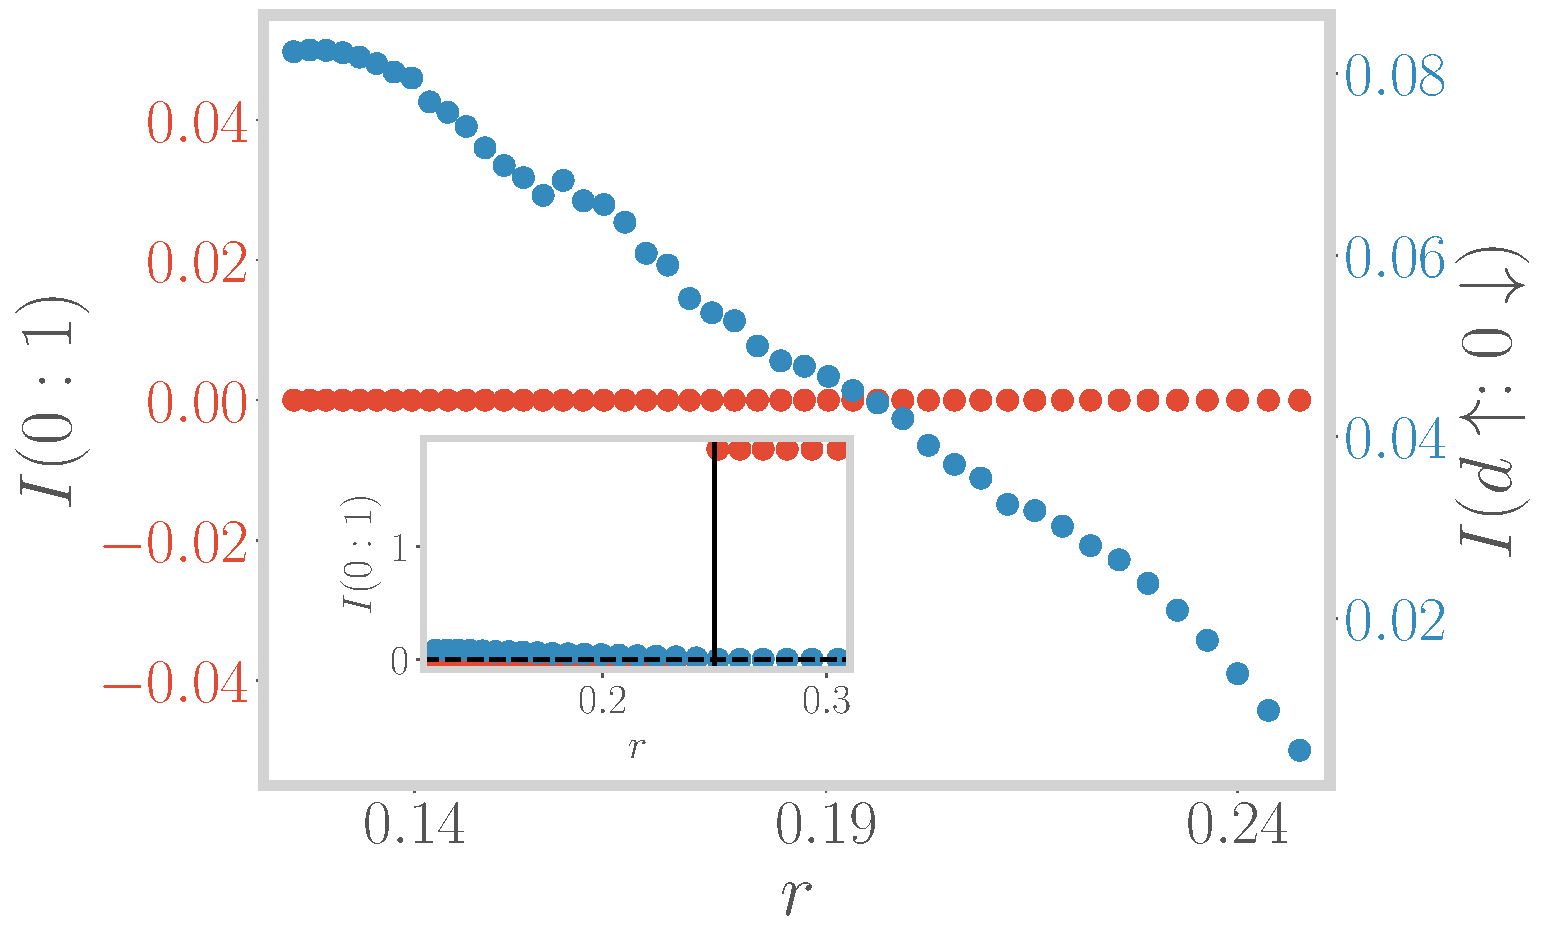
\includegraphics[width=0.45\textwidth]{I_r.pdf}
\end{frame}

\begin{frame}{Growth of pairing fluctuations in the bath}
\centering
\alert{Subdominant pairing fluctuations}, near the transition...

\vspace*{\fill}

\begin{minipage}{0.42\textwidth}
\begin{itemize}
	\nitem growth of fluctuations in Cooper channel, at the cost of spin-flip fluctuations
\end{itemize}
\end{minipage}
\hspace*{\fill}
\begin{minipage}{0.4\textwidth}
\begin{itemize}
	\nitem mutual information within the bath maximised after transition
\end{itemize}
\end{minipage}

\vspace*{\fill}

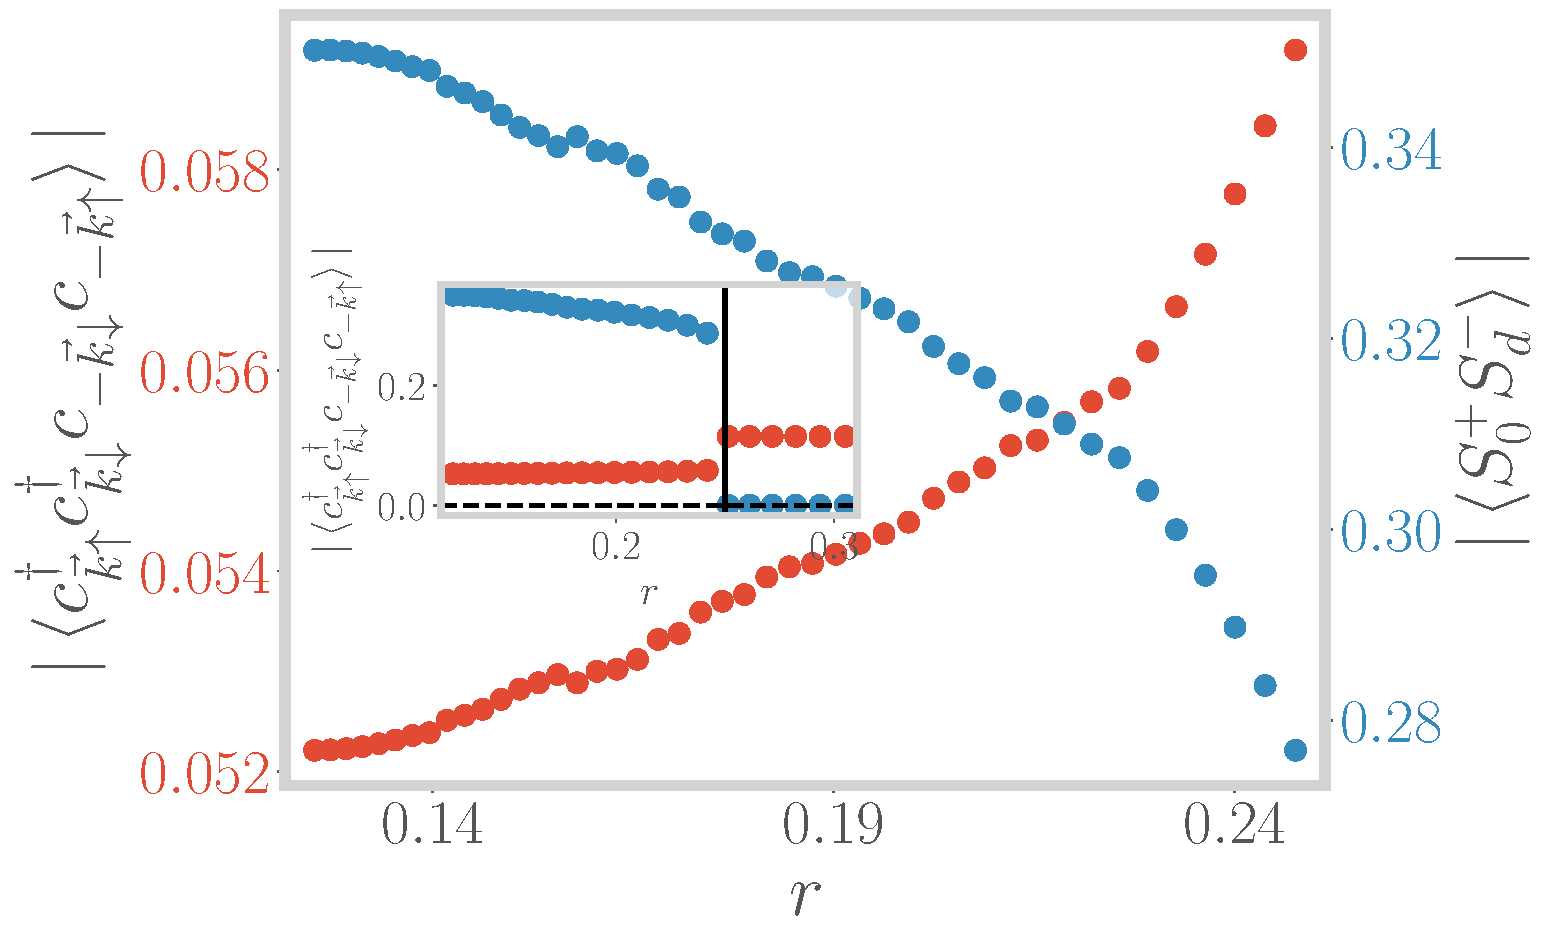
\includegraphics[width=0.45\textwidth]{spinflip-pairing.pdf}
\hspace*{\fill}
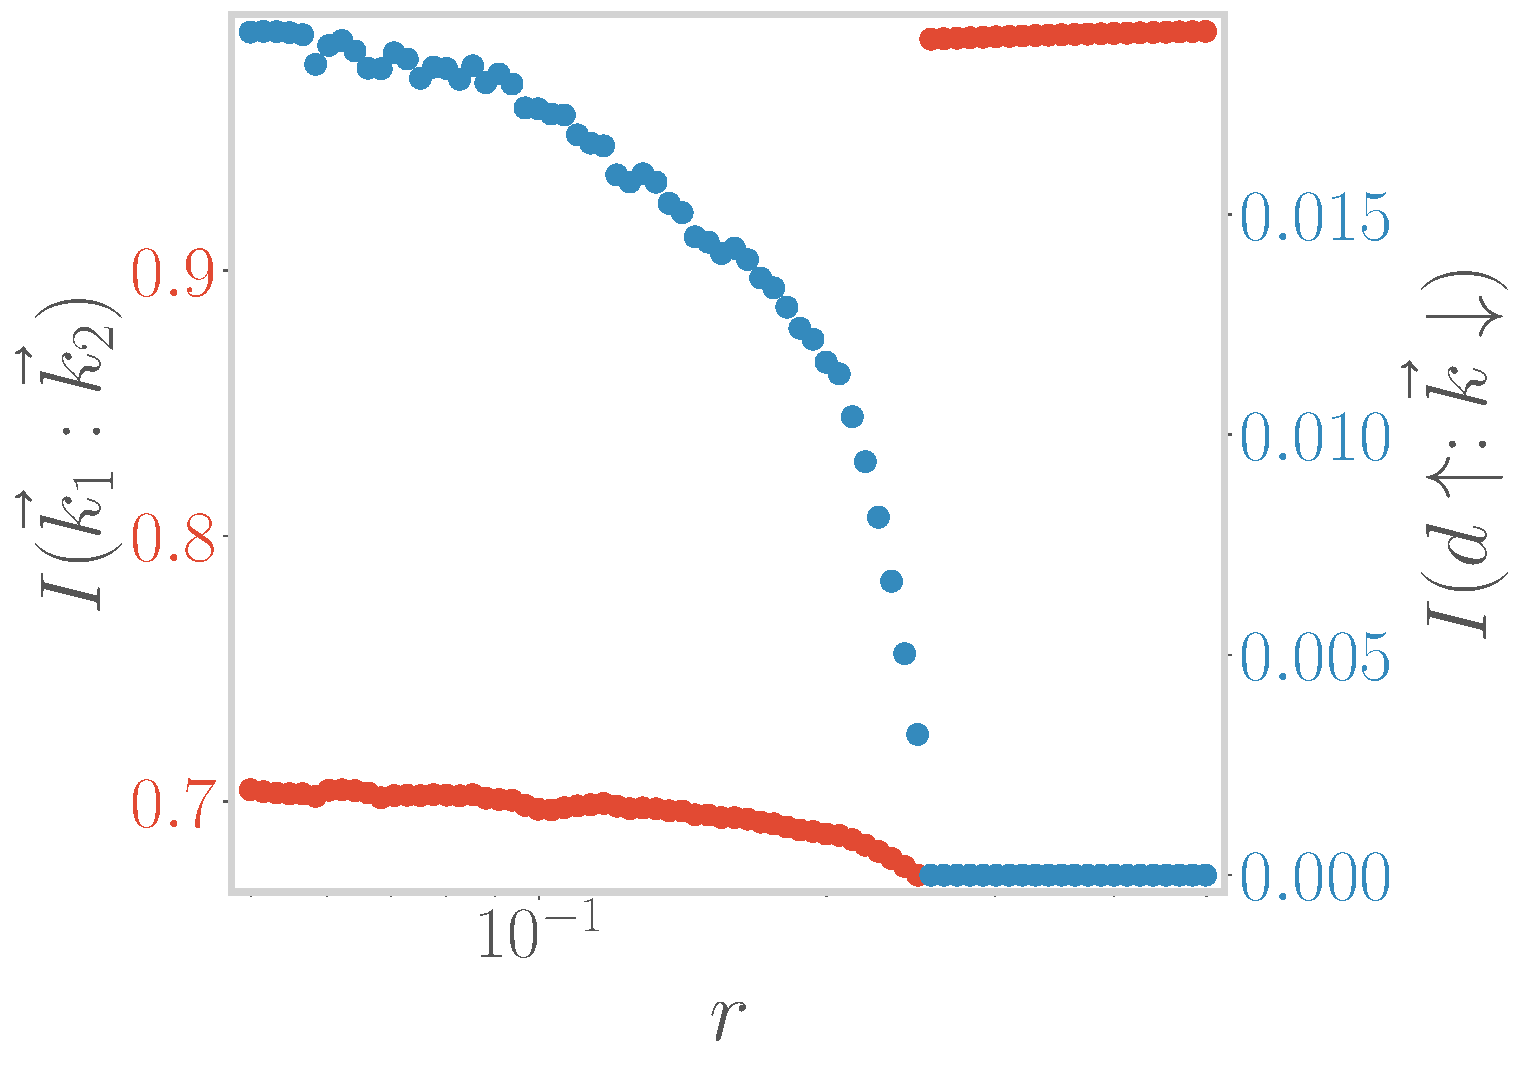
\includegraphics[width=0.45\textwidth]{I_k.pdf}
\end{frame}

\begin{frame}{}
\section{Universal Theory near the Transition}
\end{frame}
\begin{frame}{Minimal effective model for the transition}
\centering
\begin{minipage}{0.65\textwidth}
\begin{itemize}
	\nitem For \(|U_b| \lesssim J/4\), central peak and side peaks are \alert{well-separated} \\[10pt]
	\nitem \alert{Integrate out} charge fluctuations through Schrieffer-Wolff transformation
\[H_\text{eff} = \tilde J \vec{S}_d\cdot\vec{S}_0 - U_b\left(\hat n_{0 \uparrow} - \hat n_{0 \downarrow}\right)^2 + H_\text{K.E.}\]
\[ \text{RG equation for } \tilde J: ~ \Delta \tilde J \sim \tilde J \left( \tilde J  + 4U_b \right) \]
\end{itemize}
\end{minipage}
\hspace*{\fill}
\begin{minipage}{0.3\textwidth}
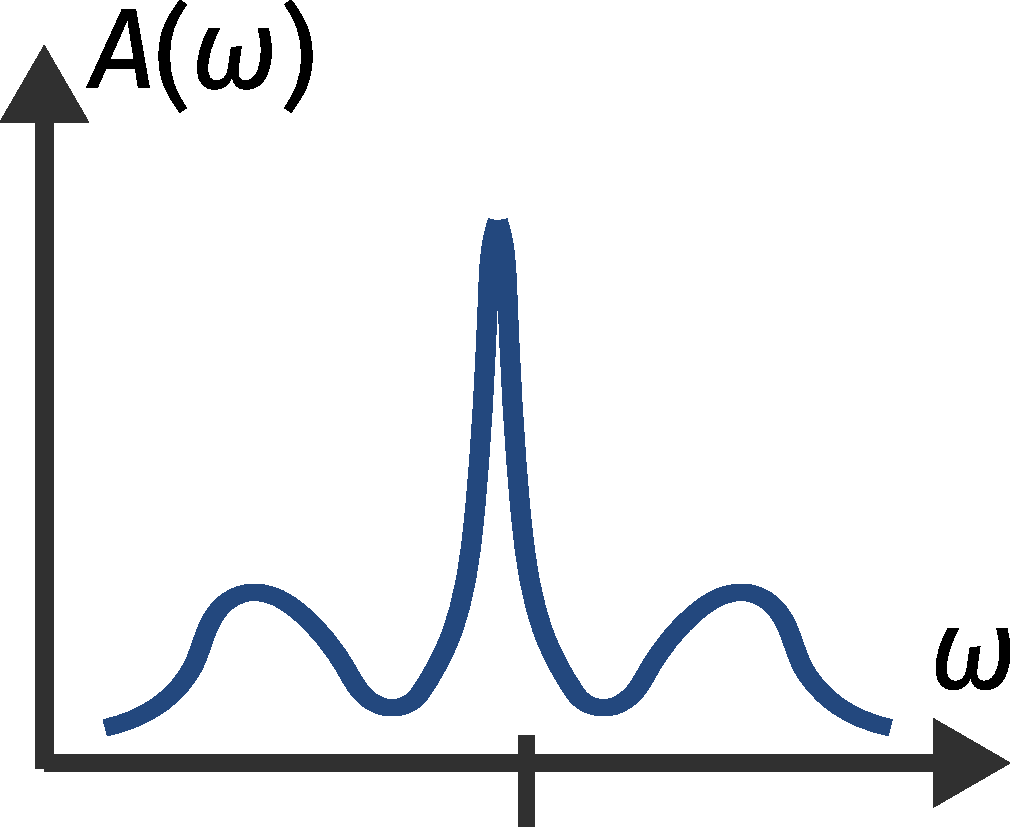
\includegraphics[width=\textwidth]{sf-2.pdf}
\end{minipage}

\begin{itemize}
\nitem \alert{captures} the criticality, and the strong-coupling and local moment phases
\end{itemize}

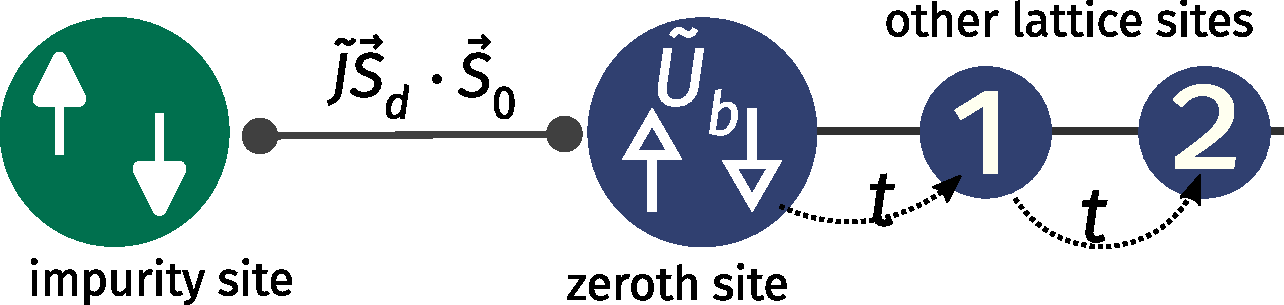
\includegraphics[width=0.7\textwidth]{universal-theory.pdf}

\vspace*{\fill}

Suggests that \alert{$J$ and $U_b$ are the minimal \& universal ingredients} for transition!

\end{frame}

\begin{frame}{Capturing the level crossing at the transition from a two-site model}

\begin{itemize}
	\nitem Obtain two-site model by taking \alert{zero bandwidth} limit\\[10pt]
	\nitem spectrum shows \alert{level crossing} between singlet and local moment states
\end{itemize}

\vspace*{\fill}

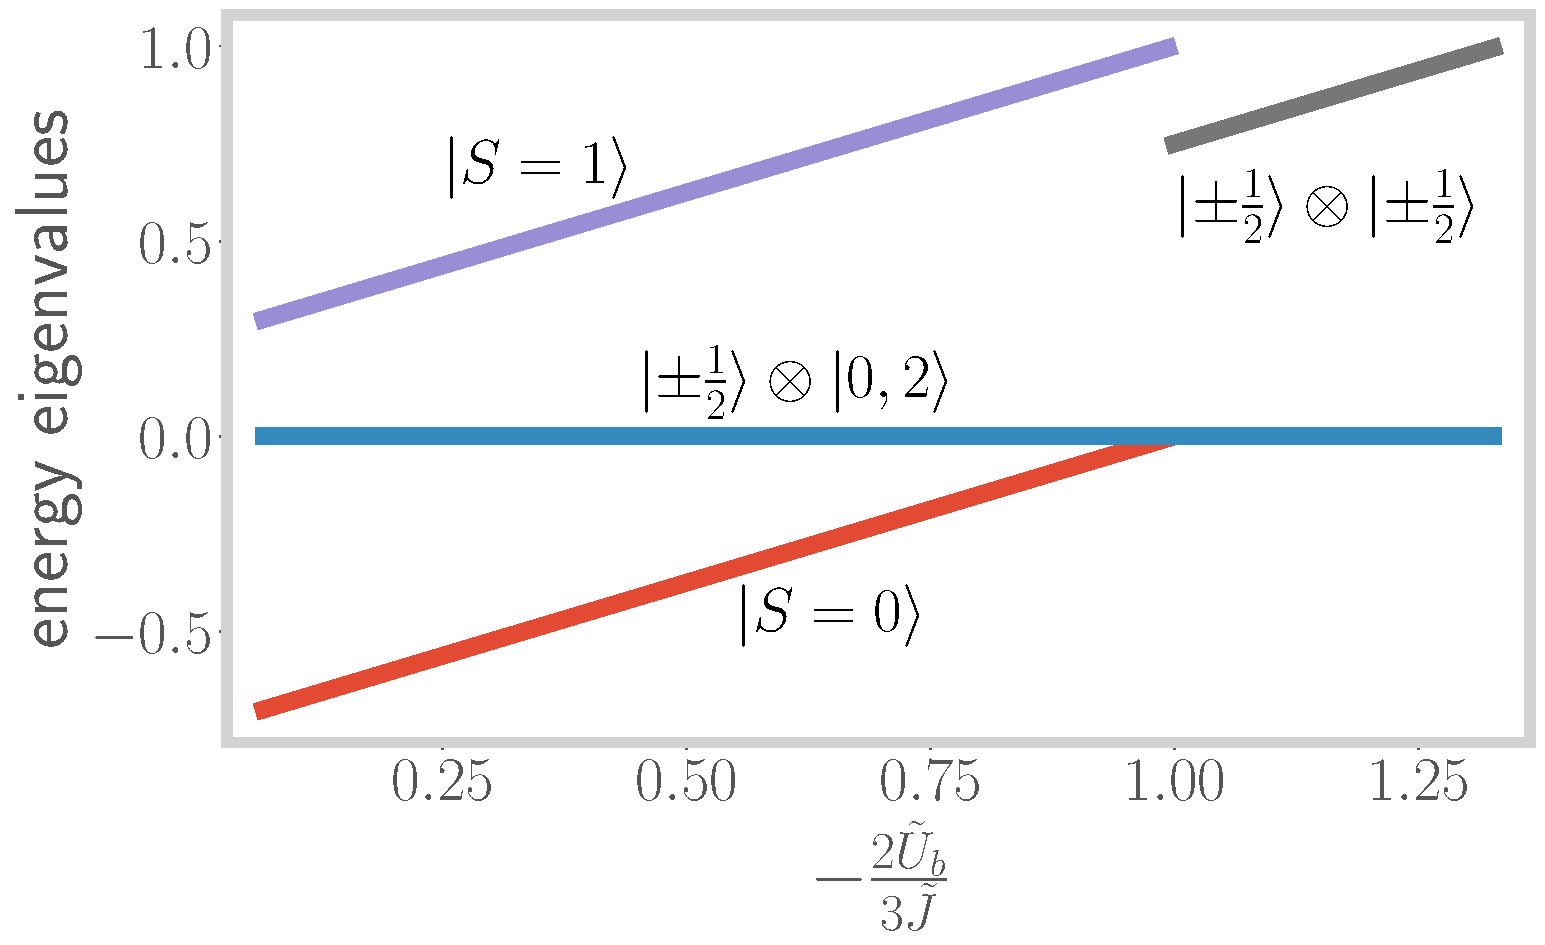
\includegraphics[width=0.5\textwidth]{twosite_spectrum.pdf}
\end{frame}

\begin{frame}{}
\section{Insights into DMFT}
\end{frame}

\begin{frame}{Extended SIAM in the context of DMFT}
\centering
\hspace*{-20pt}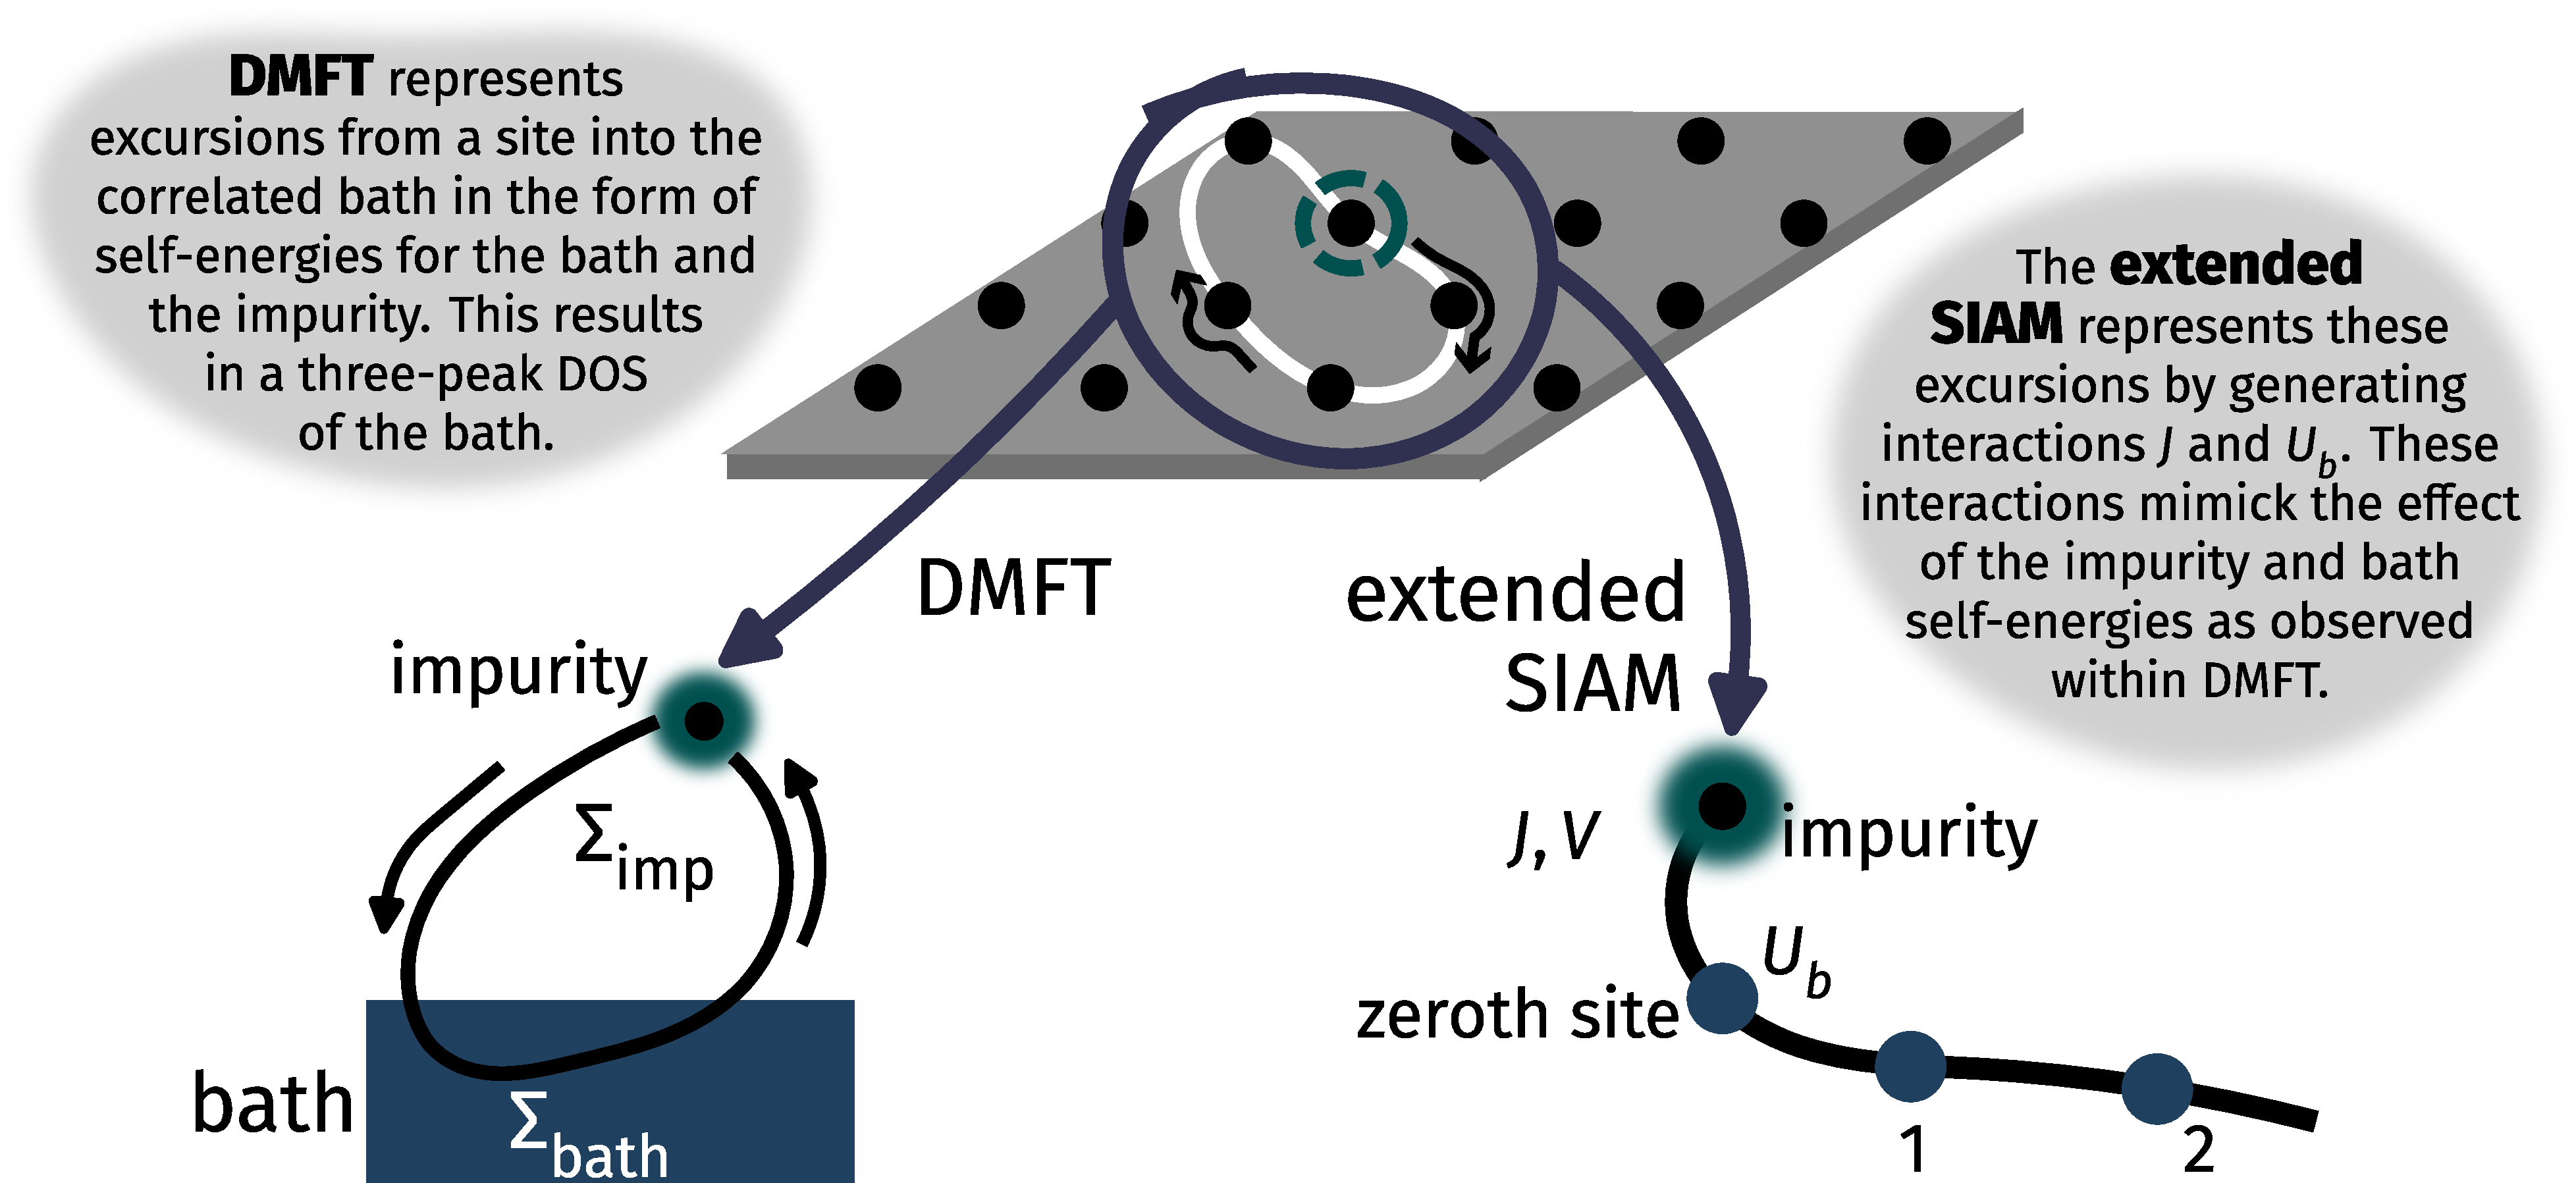
\includegraphics[width=1.1\textwidth]{contrast.pdf}
	
\end{frame}
\begin{frame}{Equivalence of the impurity site and the bath zeroth site}
\footcite{moeller_1995}
\begin{itemize}
\only<1>{
	\nitem \alert{Integrate out impurity site} from fixed point Hamiltonian via a single URG transformation\\[10pt]
\nitem Generates additional correlation $U_0$ on zeroth site
\vspace*{\fill}
\begin{center}
	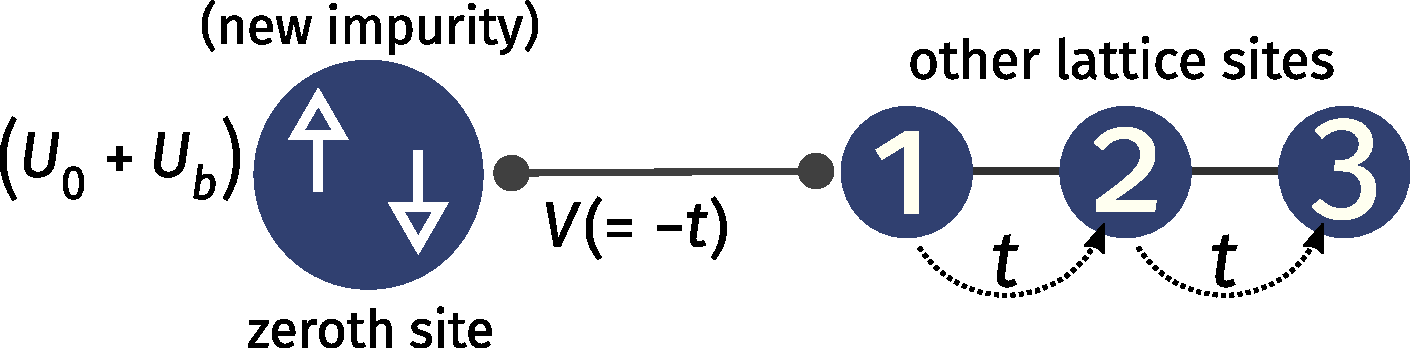
\includegraphics[width=0.6\textwidth]{decouple-impurity.pdf}\\[10pt]
\end{center}
\nitem \(J\) is relevant and the largest scale \(\longrightarrow\) \alert{repulsive correlation}:
\[U_0 + U_b \simeq J > 0\]
}
\only<2>{
\nitem \(J\) acts a \alert{symmetrisation mechanism} between impurity and zeroth sites\\[10pt]
\nitem \alert{Coherent} spin-flip scatterings ensure similarity of spectral functions\\[10pt]
\begin{center}
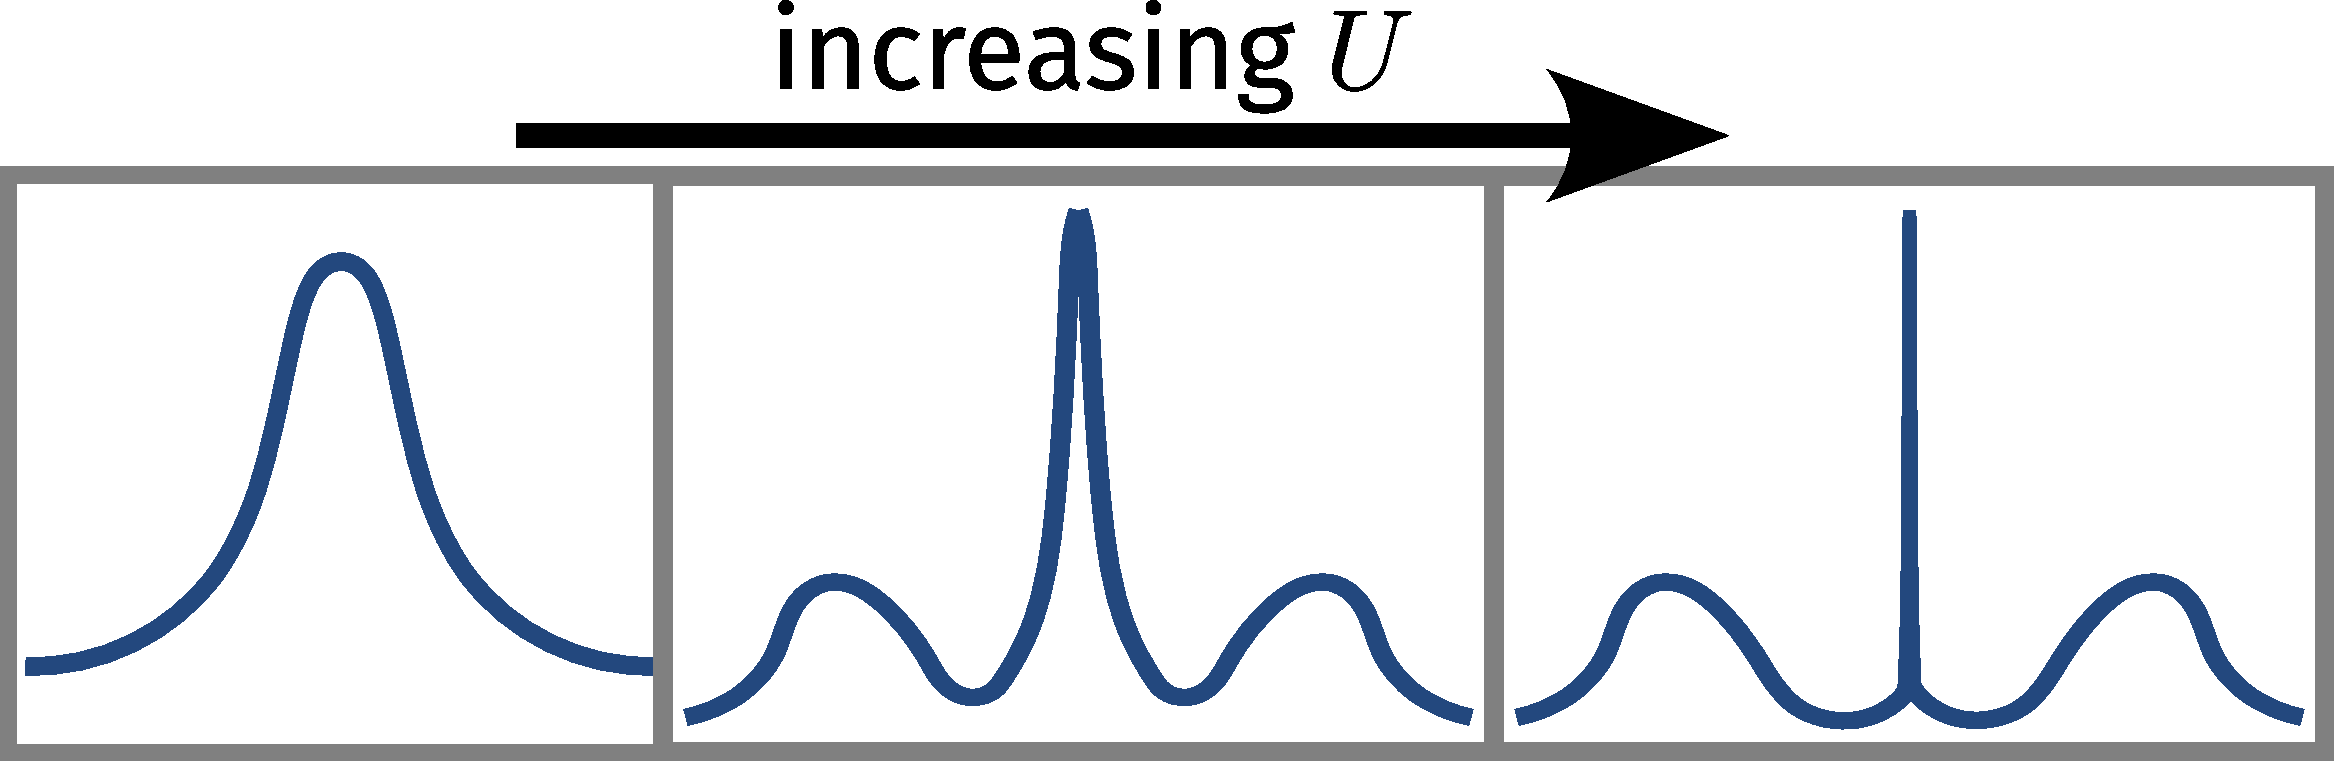
\includegraphics[width=0.5\textwidth]{standard-siam.pdf}\\[5pt]
\end{center}
}
\end{itemize}
\only<2>{
\vspace*{\fill}
{\bf \large Essence of \alert{self-consistency}: Equivalence of impurity and zeroth sites!}
}
\end{frame}


\begin{frame}{Observation of a coexistence region}
\only<1>{
\begin{itemize}
\begin{minipage}{0.45\textwidth}
\nitem DMFT observes a \alert{coexistence region} near the critical point, for \(U_{c1} < U < U_{c2}\)\\[10pt]
\nitem Insulating when coming in from the insulator, metallic when coming in from the metal
\end{minipage}
\hspace*{\fill}
\begin{minipage}{0.49\textwidth}
\begin{center}
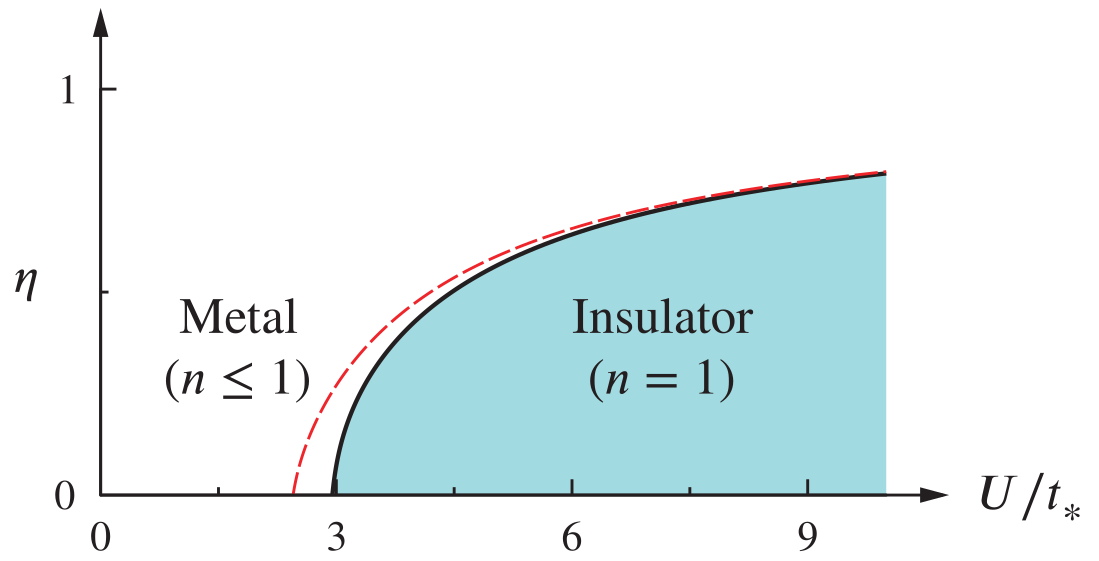
\includegraphics[width=\textwidth]{coexistence.png}\\
\footnotesize{(D.E. Logan and M.R Galpin 2016 JPCM 28 025601) }\\[10pt]
\end{center}
\end{minipage}

\vspace*{\fill}

\nitem \alert{True} transition believed to occur at \(U_{c2}\)\\[10pt]
\nitem Mott gap appears discontinuously after the transition
\end{itemize}
}
\only<2->{
{\bf \large \alert{Can be explained} heuristically using the two site spectrum}\\[10pt]
\vspace*{\fill}
\begin{itemize}
\only<2>{\nitem Initial point is when the side peaks get separated (near-zeroes in the spectral function)}
\only<3>{\nitem \(U_{c2}\) is the point where the levels cross}
\only<4>{\nitem Coming from \(U > U_{c2}\), \alert{adiabatic continuity} allows DMFT to stay on the local moment state...}
\only<5>{\nitem For \(U < U_{c1}\), local moment state is too unstable, \alert{relaxes} to the true ground state.}
\only<6>{\nitem For \(U > U_{c1}\), charge sector separated by large \(U\), leads to the \alert{discontinuous} appearance of finite gap}
\end{itemize}

\vspace*{\fill}
\begin{center}
\only<2>{
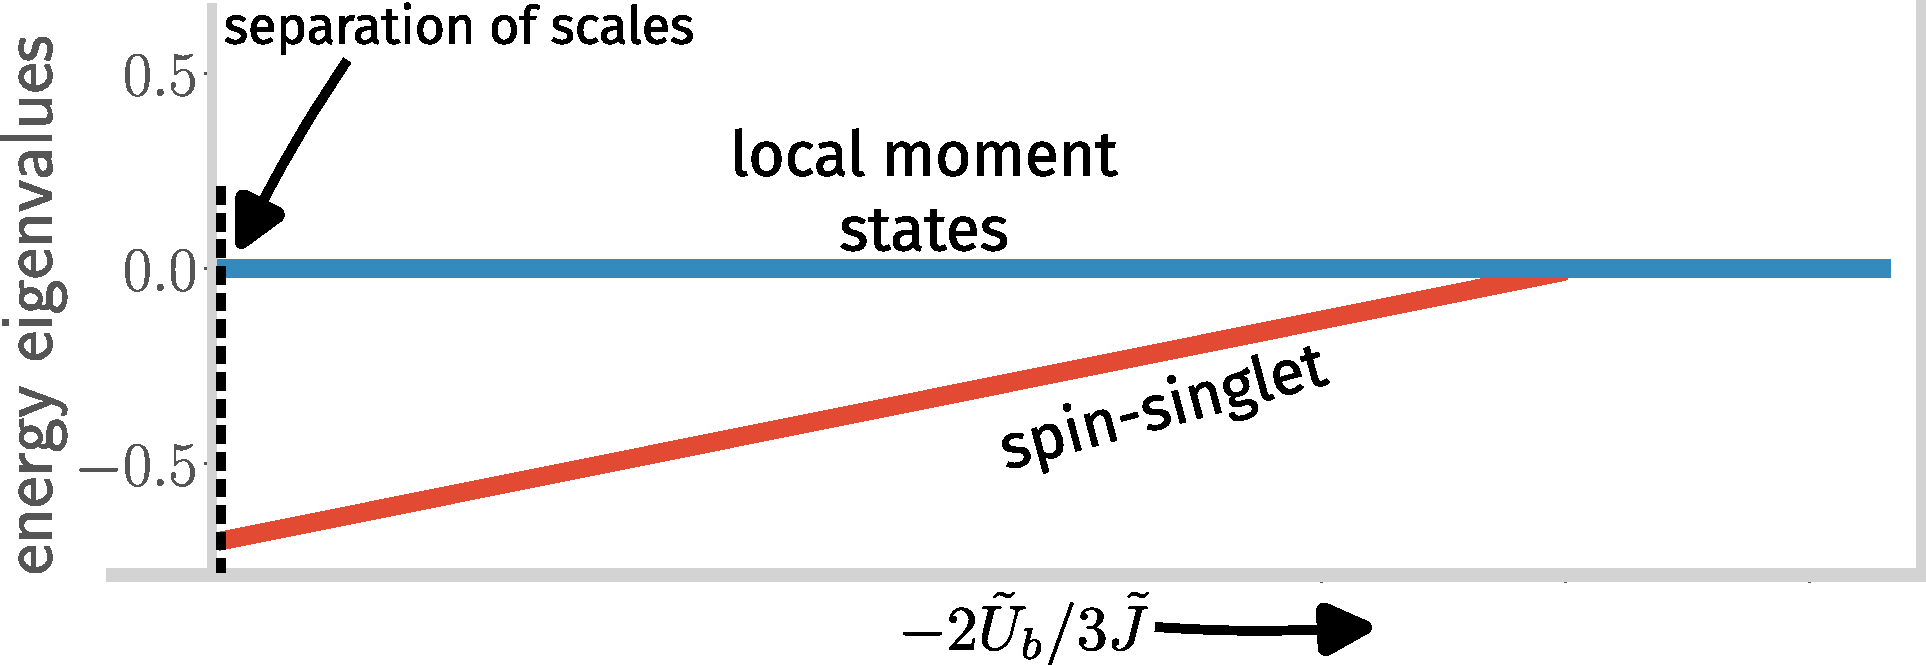
\includegraphics[width=0.6\textwidth]{coexistence-explain.pdf}
\hspace*{\fill}
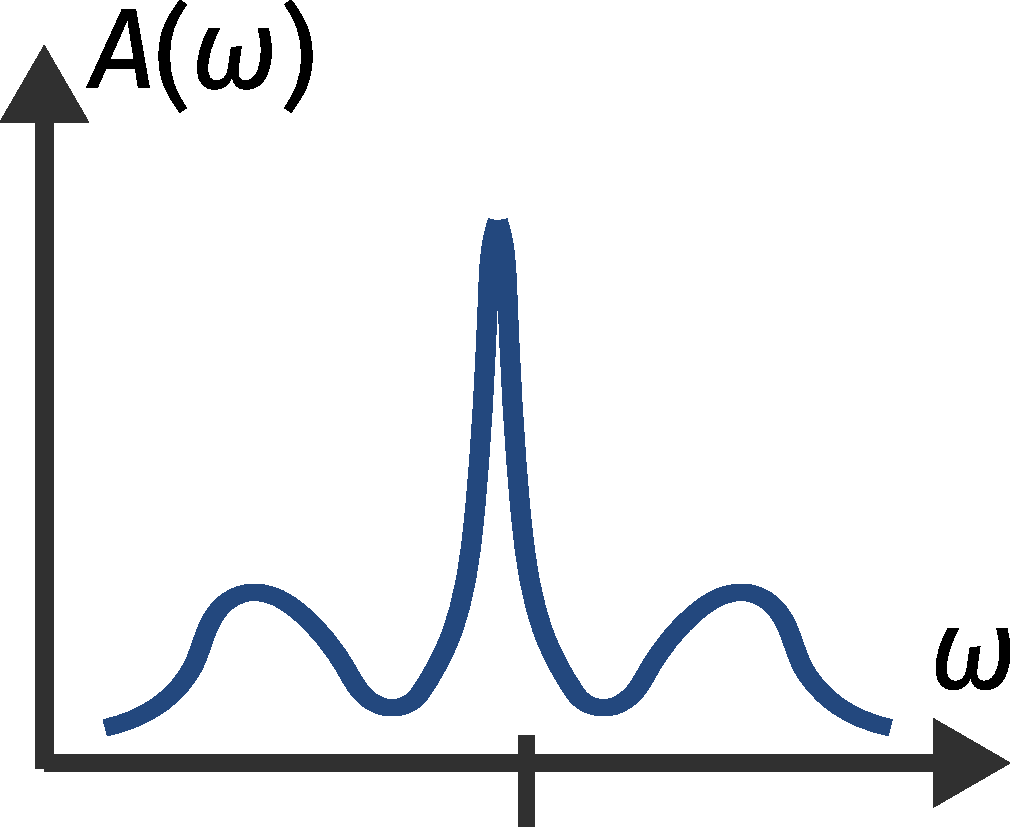
\includegraphics[width=0.25\textwidth]{sf-2.pdf}
}
\only<3>{
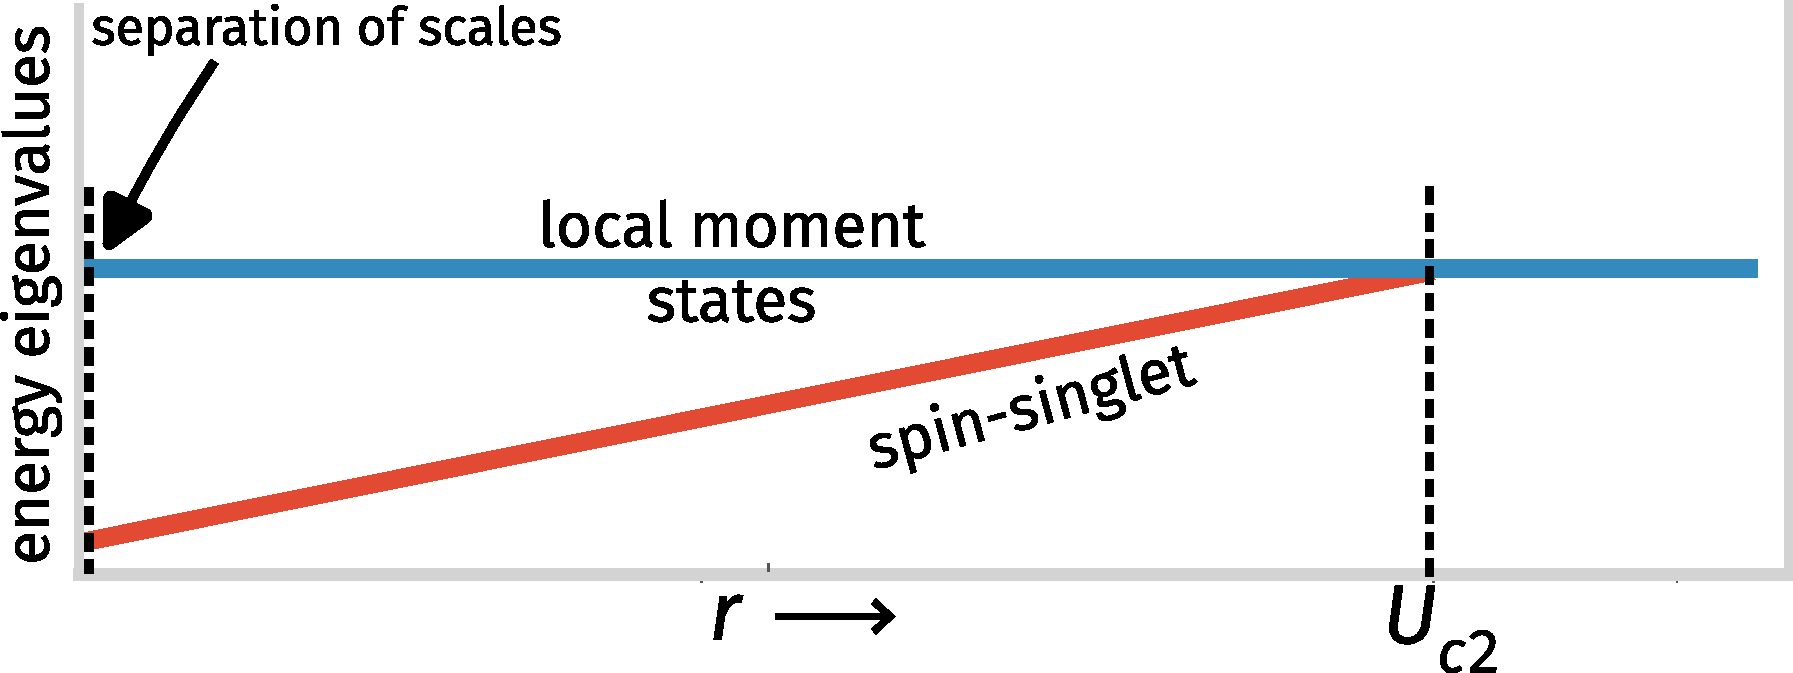
\includegraphics[width=0.6\textwidth]{coexistence-explain1.pdf}
\hspace*{\fill}
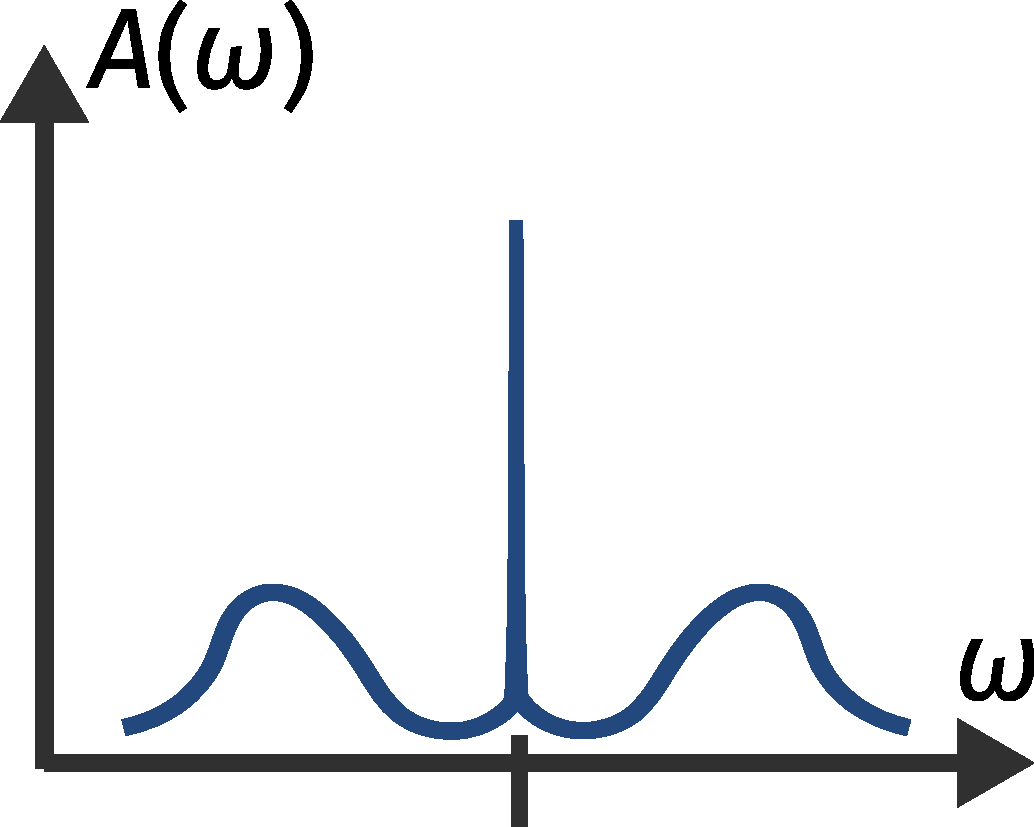
\includegraphics[width=0.25\textwidth]{sf-3.pdf}
}
\only<4>{
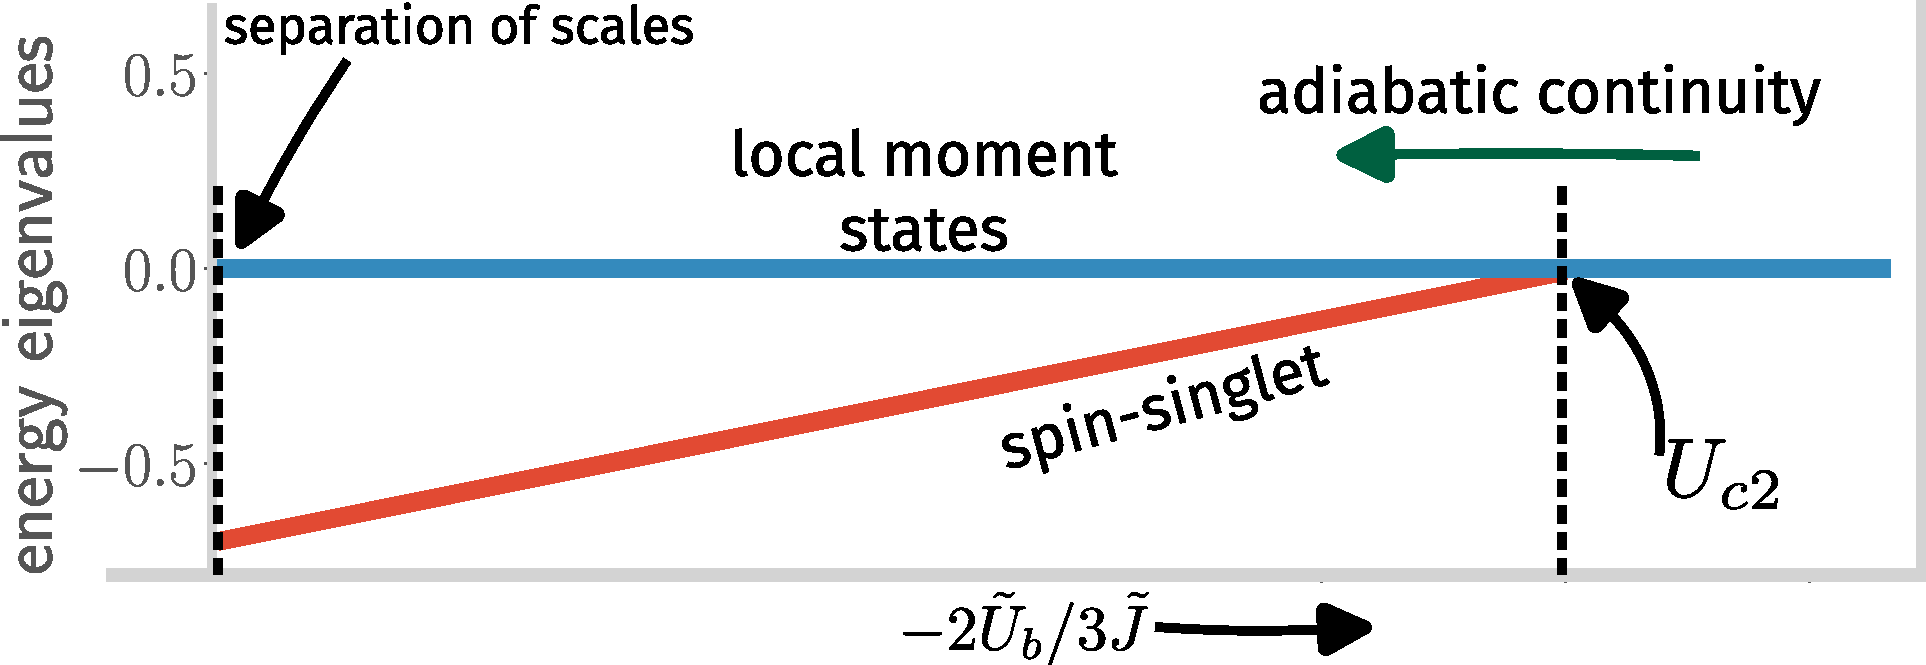
\includegraphics[width=0.6\textwidth]{coexistence-explain2.pdf}
\hspace*{\fill}
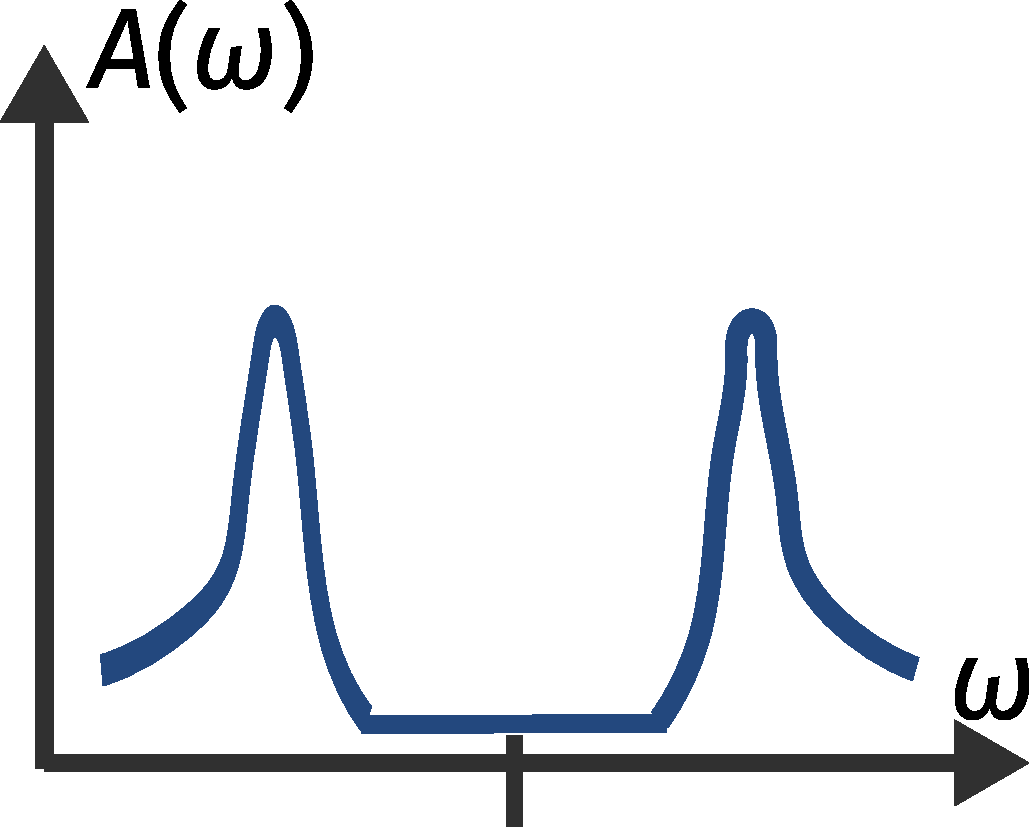
\includegraphics[width=0.25\textwidth]{sf-4.pdf}
}
\only<5>{
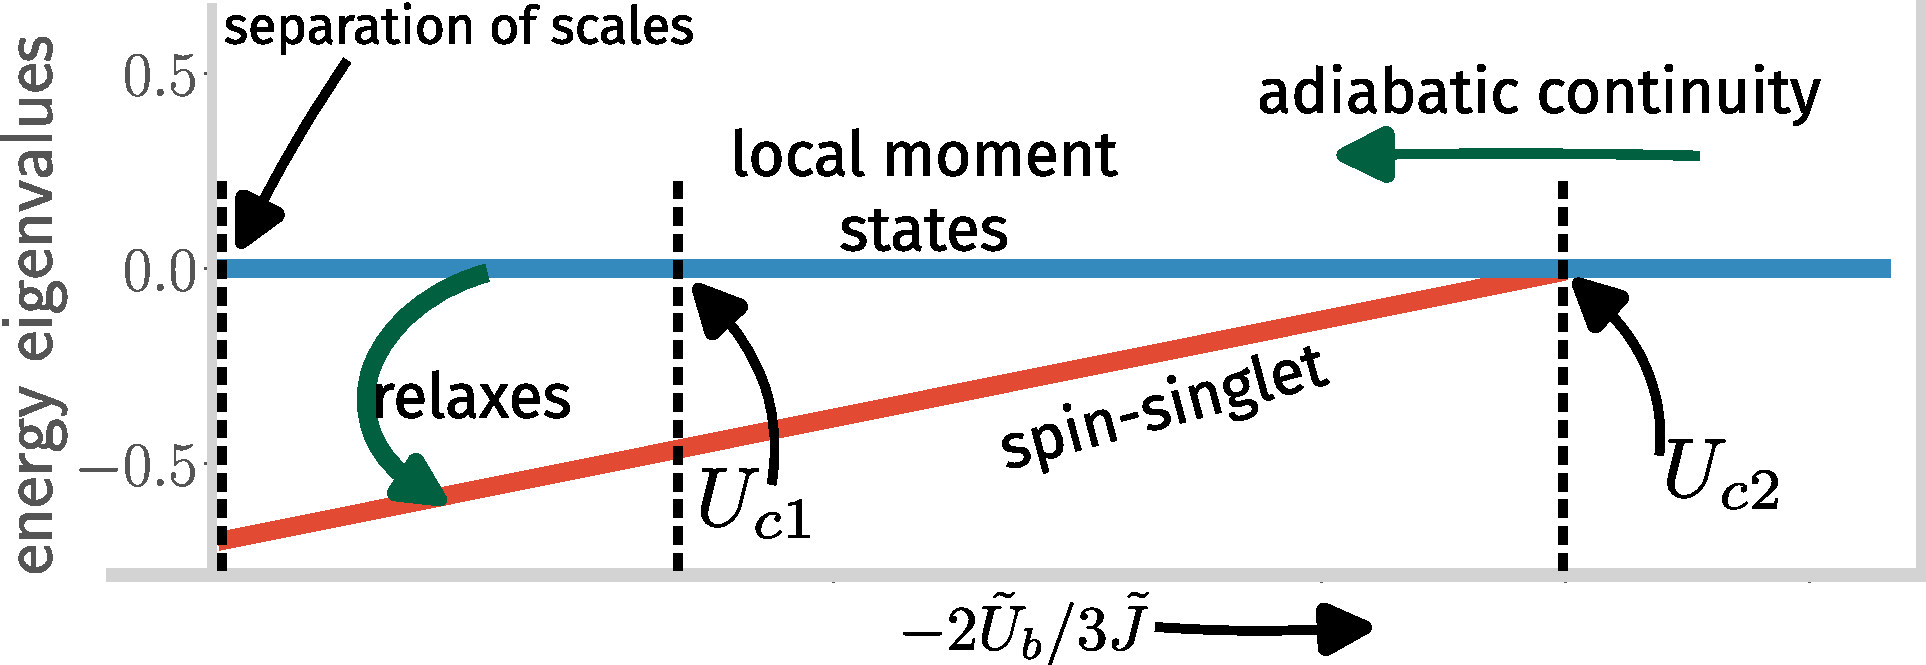
\includegraphics[width=0.6\textwidth]{coexistence-explain3.pdf}
\hspace*{\fill}
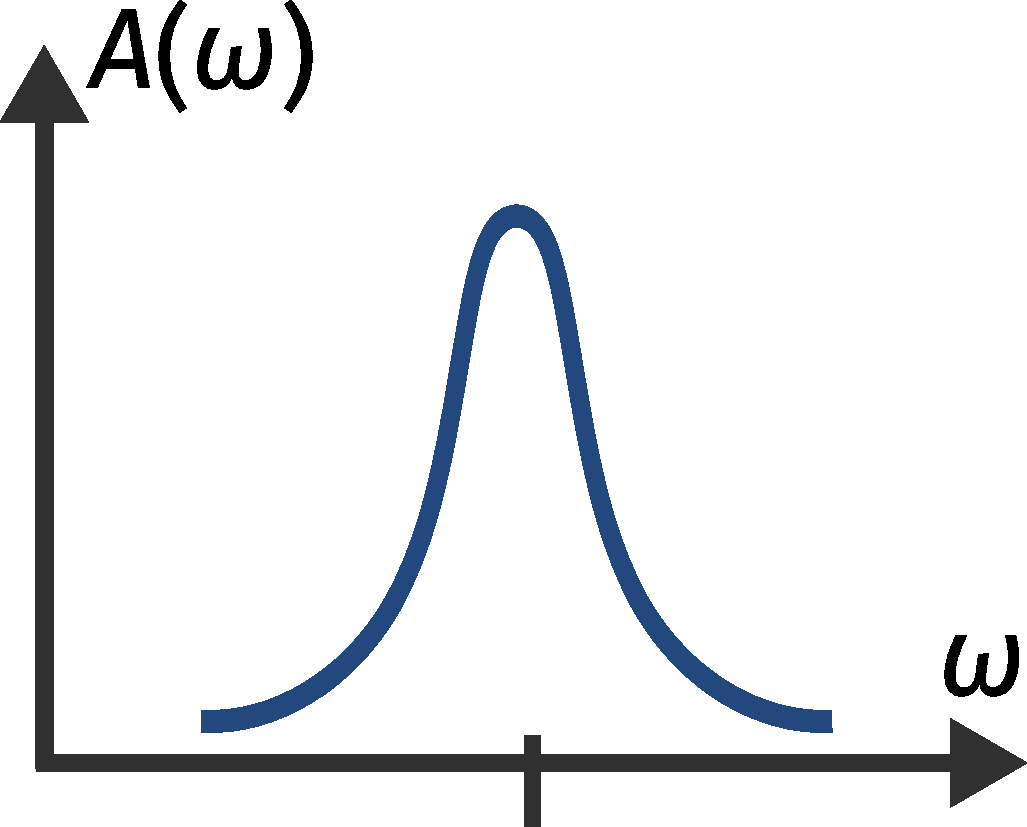
\includegraphics[width=0.25\textwidth]{sf-1.pdf}
}
\only<6>{
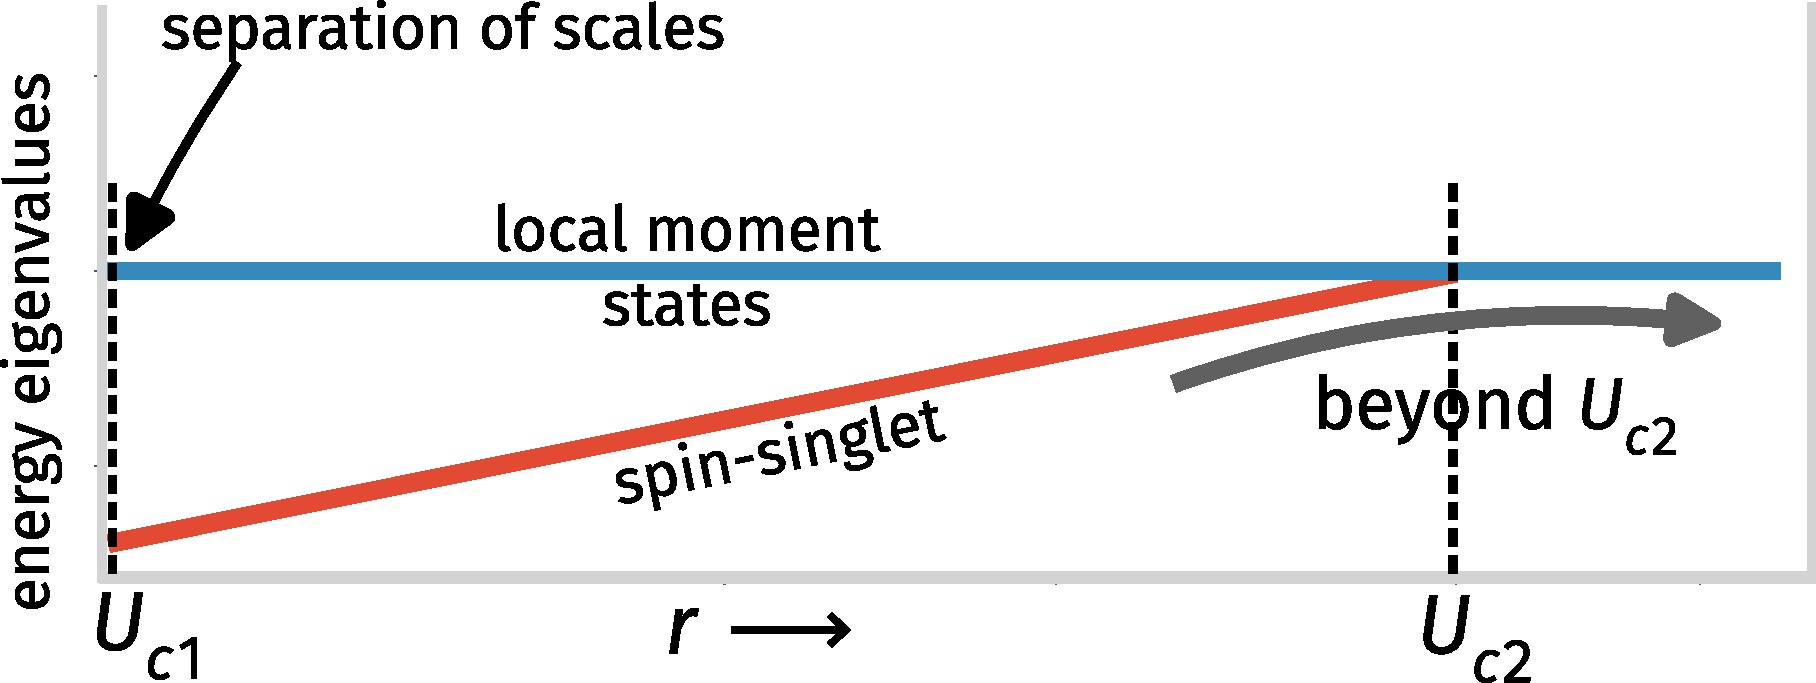
\includegraphics[width=0.6\textwidth]{coexistence-explain4.pdf}
\hspace*{\fill}
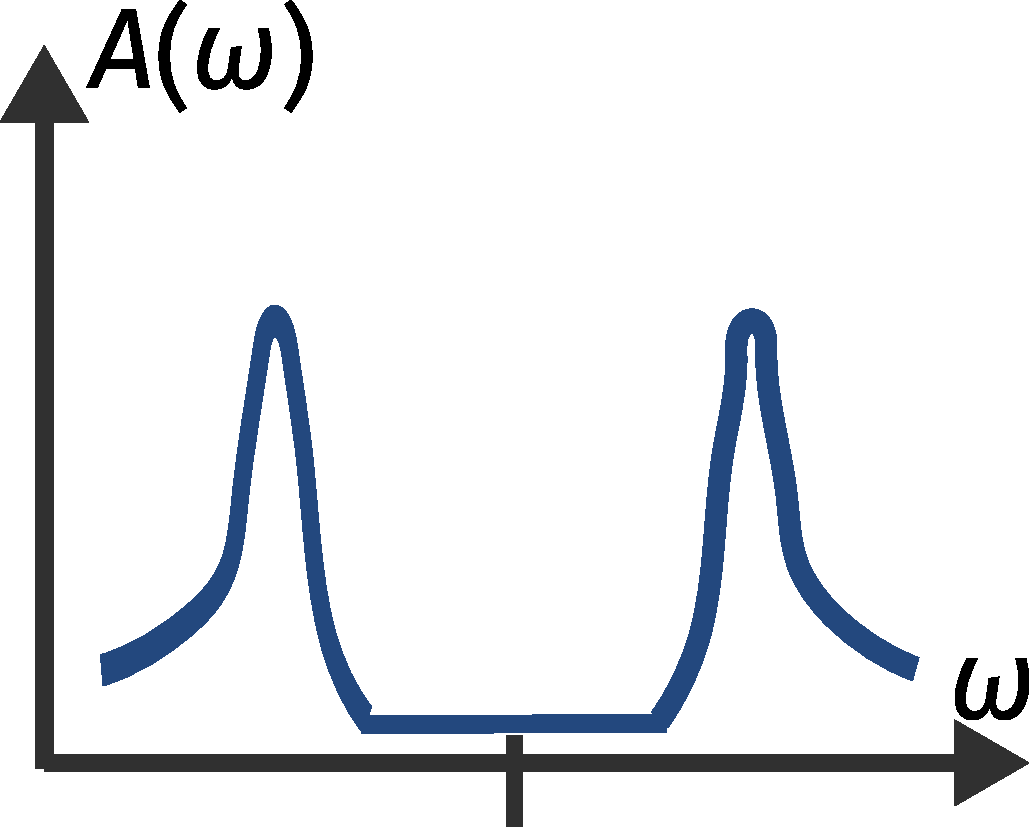
\includegraphics[width=0.25\textwidth]{sf-4.pdf}
}
\end{center}
}
\end{frame}

\begin{frame}{Comparison against NRG-DMFT correlation functions}
\only<1>{
\large{\alert{Poor Man's scaling} of the effective Kondo model}\hspace*{\fill}\small{\it [K. Held, R. Peters, and A. Toschi. PRL 2013]}\\[10pt]
\begin{itemize}
\nitem shows \alert{quantitative} agreement with NRG-DMFT (crossover scale and kinks in self-energy)\\[5pt]
\nitem Suggests that the minimal model can capture \alert{spin susc.}\\[10pt]
\begin{center}
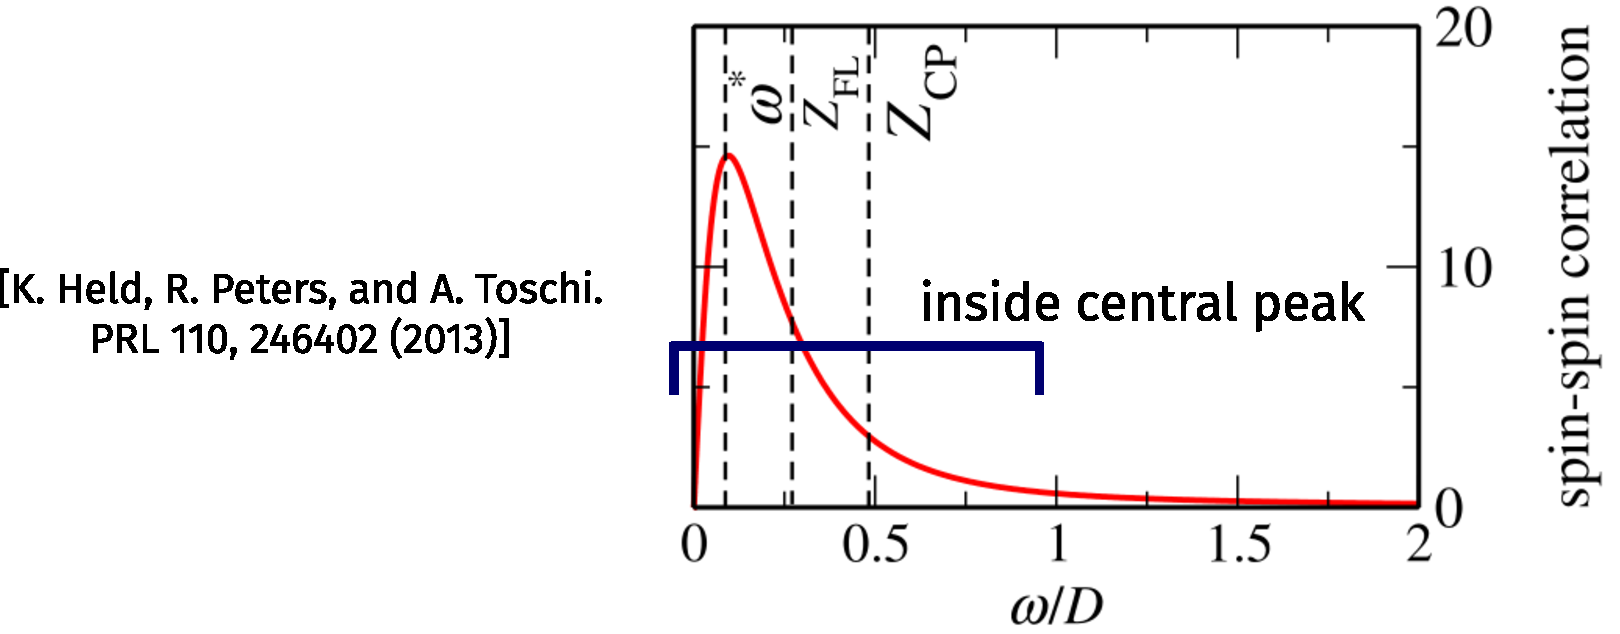
\includegraphics[width=0.5\textwidth]{spin-sus.pdf}\\[5pt]
\end{center}
\nitem Our \(J-U_b\) model \alert{goes further} by capturing physics beyond the transition
\end{itemize}
}
\only<2>{
\large{\alert{Doublon-holon correlators} of the Hubbard model}\hspace*{\fill}\small{\it [S. B. Lee, J. v Delft, and A. Weichselbaum. PRL 2017]}\\[10pt]
\begin{minipage}{0.3\textwidth}
Lee et. al show \alert{peaks} in \\[5pt]
doublon-holon correlators\\[5pt]
near zero energy \\[5pt]
within the central peak.
\end{minipage}
\hspace*{\fill}
\begin{minipage}{0.65\textwidth}
\begin{center}
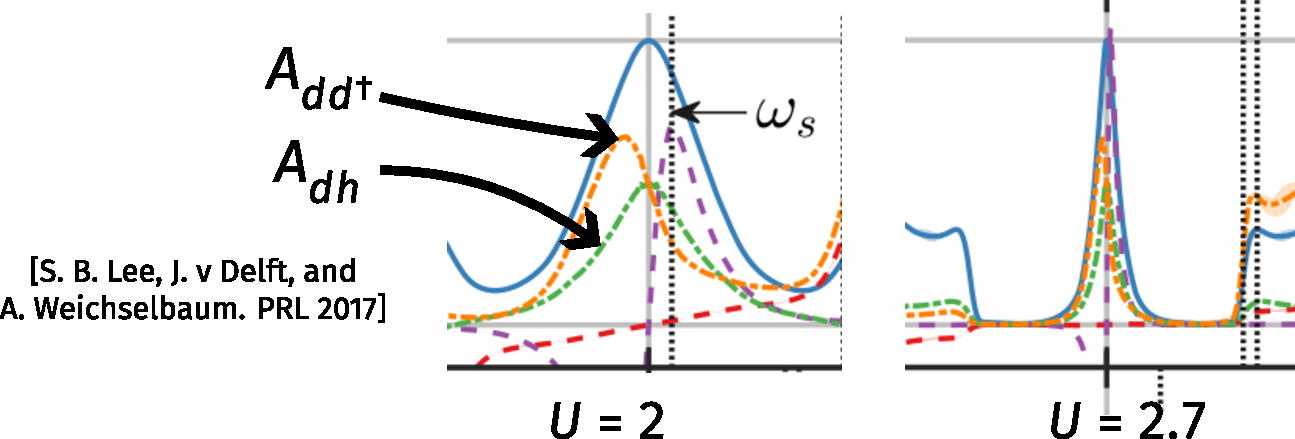
\includegraphics[width=\textwidth]{doublon-holon-correlators.pdf}
\end{center}
\end{minipage}

We find support for this in the form of \alert{increasing ground-state charge correlations and overlap}.\\[5pt]
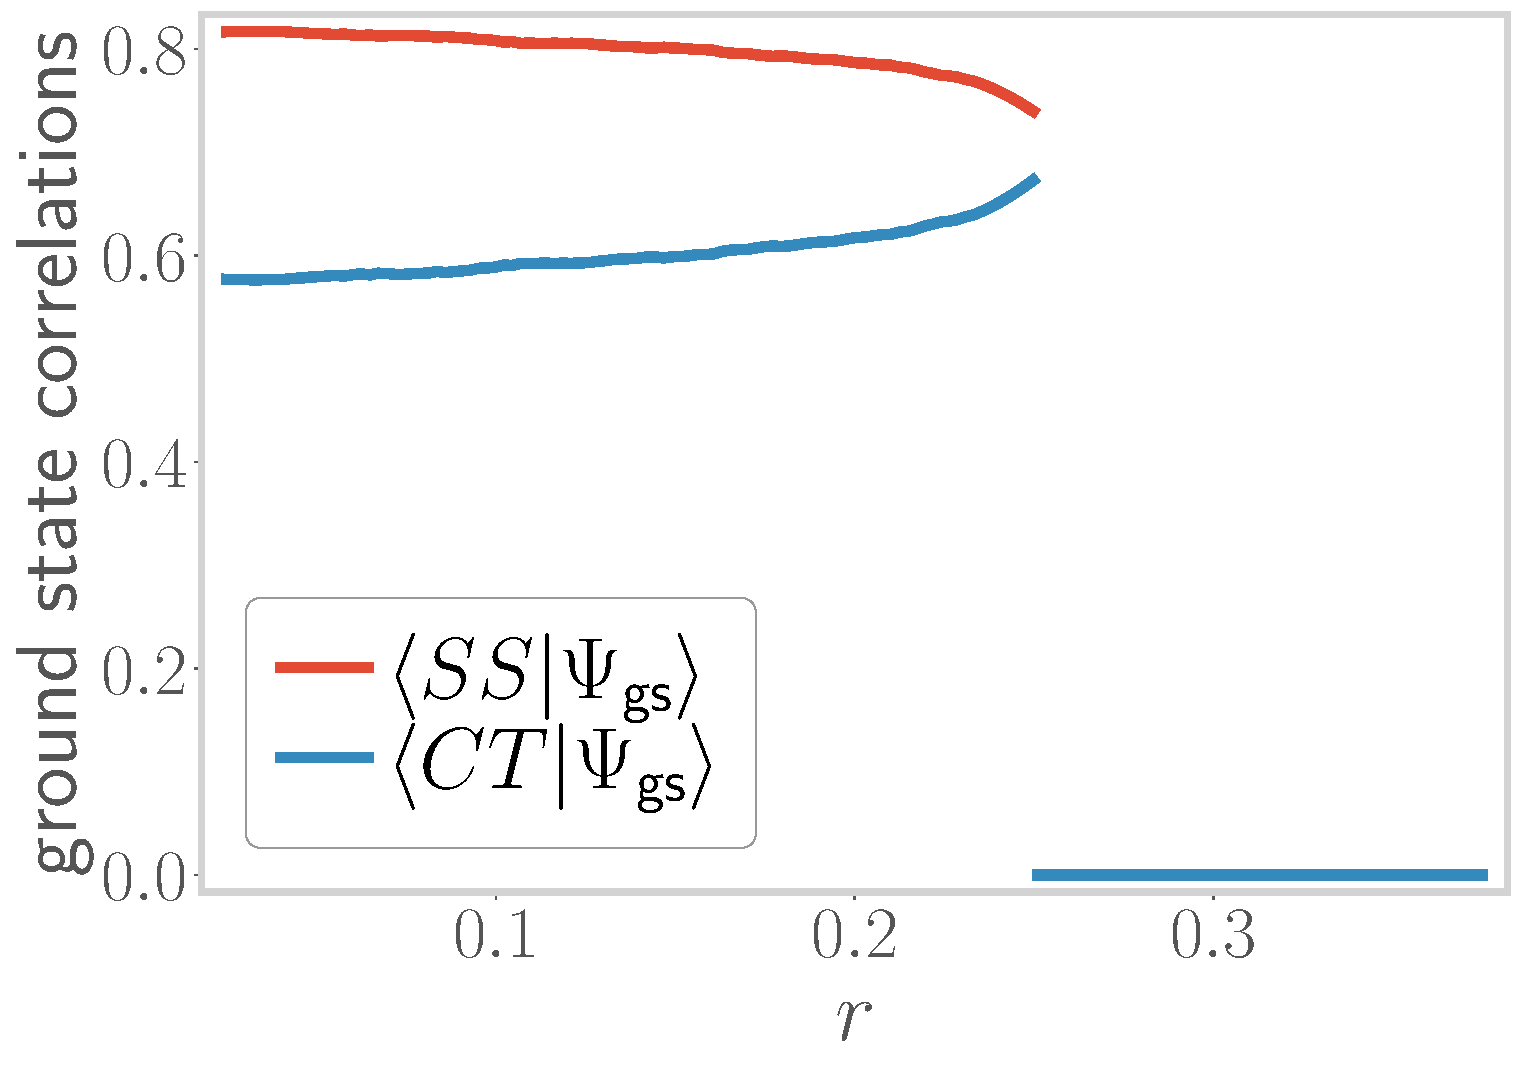
\includegraphics[width=0.4\textwidth]{corrs_gs.pdf}
\hspace*{\fill}
\includegraphics[width=0.4\textwidth]{pairing.pdf}
}
\end{frame}

\begin{frame}{}
\section{Low-energy excitations of the bath}
\end{frame}

\begin{frame}{Effect on the local Fermi liquid}
What about the \alert{low-energy excitations} of the bath, that lie above the singlet ground state?
\begin{itemize}
\nitem treat hopping between singlet and bath as perturbation 
\begin{center}
\includegraphics[width=0.6\textwidth]{perturbation.pdf}
\end{center}
\nitem Up to fourth order, charge sector becomes repulsive...
	\[H_\text{eff} = \frac{2t^4}{\tilde J\left(3\tilde J/4 + \tilde U_b \right)^2}\left[\hat n_{1 \uparrow}\hat n_{1 \downarrow} + \text{p-h}\right]  + H_\text{K.E.}\]
\nitem FL term blows up towards transition, signaling \alert{breakdown} of Fermi liquid theory and loss of adiabaticity.
\end{itemize}
\end{frame}

\begin{frame}{Effect on the local Fermi liquid}
\footcite{held_2013}
Vanishing of the \alert{Kondo scale} \(T_K\) towards the transition
\vspace*{\fill}

\begin{itemize}
	\nitem Kondo temperature scale $T_K$ can be obtained from the \(J-U_b\) model, but with a Lorentzian DOS in the bath, \(\rho = \rho_0 \Gamma^2/(D^2 + \Gamma^2)\).\\[10pt]
	\nitem Near the transition \(r = -U_b/J_0 \to \frac{1}{4}\), the fixed-point momentum energy scale \(D^*\) can be approximated as
	\[D^* = D_0 \exp \left[\frac{\left( 2\omega + U_b + J_0/2 \right)^2}{8U_b\rho_0 \Gamma^2}\ln |1 - 4r|\right], ~ ~ D_0 = \text{UV cutoff}~.\]\\[5pt]
	\nitem Kondo temperature can be defined as \(T_K = \hbar \Lambda^*/k_B\), vanishes towards the critical point
	\[T_K = \frac{D_0}{k_B} \exp \left[\frac{\left( 2\omega + U_b + J_0/2 \right)^2}{8U_b\rho_0 \Gamma^2}\ln |1 - 4r|\right]\]
\end{itemize}
\end{frame}

\begin{frame}{Effect on the local Fermi liquid}
	How do the imaginary part of \alert{self-energy} \(\Sigma\) and the \alert{quasiparticle residue} behave near the transition?
	\vspace*{\fill}

\begin{itemize}
	\nitem Following the renormalised perturbation theory approach of Hewson~\footcite{hewson1993,coleman2015}, \(\text{Im}\left[\Sigma(\omega)\right] \) is
	\[\text{Im}\left[\Sigma(\omega)\right] \sim u^2 \omega^2, ~ ~ u = \frac{2t^4}{\tilde J\left(3\tilde J/4 + \tilde U_b \right)^2}\]
	\nitem As \(r \to 0\), \(u \to \infty\), signalling a vanishing lifetime of the quasiparticles\\[10pt]
	\nitem Quasiparticle residue \(Z\) for 1-particle excitations is proportional to \(T_K\):
	\[Z \sim T_K\]
	\[Z \to 0 \text{ as }r \to 0\]
\end{itemize}
\end{frame}


\begin{frame}{Broad conclusions}
\begin{itemize}
	\nitem The extended SIAM appears to capture the DMFT transition and \alert{self-consistency}.\\[10pt]
	\nitem The key ingredient is a \alert{competition} between Kondo screening physics and a local attractive correlation in the bath.\\[10pt]
	\nitem Crucial feature of the journey is the enhancement of \alert{pairing fluctuations} in the bath - leads to destruction of Kondo cloud.\\[10pt]
	\nitem An emergent self-consistency is achieved through the qualitative similarity of the spectral functions of the impurity and zeroth sites.\\[10pt]
	\nitem  SOMETHING ABOUT THE FINAL CALCULATIONS (MAYBE NON-FERMI LIQUID PHYSICS)
\end{itemize}	
\end{frame}

\begin{frame}{}
\section{Future Prospects}
\end{frame}

\begin{frame}{Future Prospects}
\begin{itemize}
	\nitem The extended SIAM can be improved by considering \alert{multiple impurities} and general impurity \alert{filling}.\\[20pt]
	\nitem We are developing a new \alert{tiling-based auxiliary model method} can used for studying other models of strong-correlations as well as topologically active or flat band systems.\\[20pt]
	\nitem The URG can be applied to \alert{heavy-fermion materials} towards a study of phase diagram and unconventional superconductivity, as well as Kondo insulators.\\[20pt]
	\nitem Interacting systems in a magnetic field is also a potential area of study, specifically \alert{fractional Chern insulators} (e.g. the fractional quantum hall effects).
\end{itemize}
\end{frame}


\begin{frame}{Acknowledgements}

\flushleft
Gracious thanks to\\[10pt]
\begin{itemize}
	\nitem my collaborators \alert{S. Patra, A. Mukherjee, Prof. A. Taraphder} and \alert{Prof. N. S. Vidhyadhiraja},\\[10pt]
	\nitem my RPC members \alert{Prof. Ritesh Singh} and \alert{Prof. Anandamohan Ghosh} for instructive feedback,\\[10pt]
	\nitem \alert{Prof. H. Casini, Prof. N. Banerjee} and \alert{Shibendu G. Chowdhury} for very fruitful discussions, and\\[10pt]
	\nitem IISER Kolkata for funding.
\end{itemize}

\end{frame}

\appendix

\begin{frame}[allowframebreaks]{References}
\printbibliography[heading=none]
\end{frame}

\begin{frame}{}
\section{Other Projects}
\end{frame}

\begin{frame}{}
\section{Theory for the single-channel Kondo cloud}
\begin{minipage}{0.55\textwidth}
	\small{{\bf Phys. Rev. B 105, 085119}\\[10pt]
Anirban Mukherjee, \alert{Abhirup Mukherjee}, N. S. Vidhyadhiraja, A. Taraphder, and Siddhartha Lal}
\end{minipage}
\hspace*{\fill}
\begin{minipage}{0.4\textwidth}
	\includegraphics[width=\textwidth]{kondo-effect.pdf}
\end{minipage}
\end{frame}

\begin{frame}{Theory for the single-channel Kondo cloud}
\footcite{kondo1964resistance,wilson1975,andreiKondoreview,hewson1993,nozieres1974fermi,anderson1970,tsvelickKondoreview,affleck1993exact,Goldhaber-Gordon1998,Borzenets2020,sakai_osamu_shimizu,costi_hewson_1990,nozaki2012,affleck1995conformal}

\begin{minipage}{0.49\textwidth}
\centering
\begin{itemize}
\nitem spectral function \& magnetic susceptibility
\end{itemize}

\vspace*{10pt}

\includegraphics[width=0.8\textwidth]{chi_parts.pdf}
\end{minipage}
\begin{minipage}{0.49\textwidth}
\centering
\includegraphics[width=0.8\textwidth]{entropy_therm.pdf}

\vspace*{10pt}

\begin{itemize}
\nitem local Fermi liq. \& orthogonality catastrophe
\nitem thermal entropy
\end{itemize}
\end{minipage}

\end{frame}

\begin{frame}{}
\section{Role of degeneracy in the multi-channel Kondo problem}
\begin{minipage}{0.55\textwidth}
	\small{{\bf arXiv:2205.00790}\\[10pt]
Siddhartha Patra, \alert{Abhirup Mukherjee}, Anirban Mukherjee, N. S. Vidhyadhiraja, A. Taraphder, Siddhartha Lal}
\end{minipage}
\hspace*{\fill}
\begin{minipage}{0.4\textwidth}
	\includegraphics[width=\textwidth]{stargraph.pdf}
\end{minipage}
\end{frame}

\begin{frame}{Role of degeneracy in the multi-channel Kondo problem}
\footcite{Noz_blandin_1980,Tsvelick_weigmann_mchannel_1985,affleck1993exact,Gan_mchannel_1994,affleck_1991_overscreen,emery_kivelson,bulla_1998}

\begin{enumerate}
	\only<1>{\nitem Intermediate-coupling RG fixed point Hamiltonian and \alert{degenerate} ground states
	\nitem Degree of compensation, magnetization and susceptibility show \alert{incomplete screening}}
	\only<2>{\nitem Local \alert{marginal Fermi liquid} within the low-energy excitations of the bath
\nitem \alert{Duality} relations constrain the RG flows of the MCK model}
\end{enumerate}
\vspace*{\fill}

\only<1>{
\includegraphics[width=0.4\textwidth]{CentralFieldChiPowerlaw.pdf}
\hspace*{\fill}
\includegraphics[width=0.4\textwidth]{discmagimpgen.pdf}
}

\only<2>{
\includegraphics[width=0.7\textwidth]{duality.pdf}
}

\end{frame}

\begin{frame}{}
\section{Entanglement scaling in free fermions: holography \& topology}

\begin{minipage}{0.3\textwidth}
	\includegraphics[width=\textwidth]{figures/Matroshka.png}
\end{minipage}
\hspace*{\fill}
\begin{minipage}{0.5\textwidth}
\includegraphics[width=\textwidth]{figures/holography.pdf}
\end{minipage}

\end{frame}

\begin{frame}{Entanglement scaling in free fermions: holography \& topology - Summary}
\hspace*{-40pt}
\begin{minipage}{0.65\textwidth}
\begin{itemize}
	\nitem Under coarse-graining or fine-graining in \(k-\)space, entanglement of free Dirac fermions shows hierarchical onion-like structure.\\[10pt]
	\nitem Entanglement scaling can be used to define distances, leads to additional spatial dimension \(\longrightarrow\) holography.\\[10pt]
	\nitem Emergent distances and curvature can be related to RG beta function; the sign of the curvature is topological.\\[10pt]
	\nitem Pole structure of the entanglement tracks the Luttinger volume - invariant under the scaling transformations.
\end{itemize}
\end{minipage}
\hspace*{5pt}
\begin{minipage}{0.41\textwidth}
\includegraphics[width=\textwidth]{figures/A_mi.pdf}
\includegraphics[width=\textwidth]{curvature-pos.pdf}
\end{minipage}
\hspace*{-40pt}
\end{frame}



\begin{frame}{Creating subsystems}
	\[\text{Free Dirac fermions on torus:}~ ~ ~ k_x^n = \frac{2\pi }{L_x} n,~ ~ n \in \mathbb{Z};~~~ \text{define \alert{sparsity}} = \Delta n = 1\]
	\alert{Simplest} choice: the entire set
	\[\text{sparsity} = 1 \longrightarrow n \in \left\{-N,-(N-1),-(N-2),\ldots,-1,0,1,\ldots,N-2,N-1,N\right\} \]
	\alert{Coarser} choices: increase sparsity
	\[\text{sparsity} = 2 \longrightarrow n \in \left\{-N,-(N-2),-(N-4),\ldots,-2,0,2,\ldots,N-4,N-2,N\right\} \]
	\[\text{sparsity} = 4 \longrightarrow n \in \left\{-N,-(N-4),-(N-8),\ldots,-4,0,4,\ldots,N-8,N-4,N\right\} \]
	\centering
	\vspace*{\fill}
	\includegraphics[width=0.4\textwidth]{figures/A_mi.pdf}
	\hspace*{\fill}
	\includegraphics[width=0.25\textwidth]{figures/subsystem-torus.pdf}
\end{frame}

\begin{frame}{Subsystem entanglement entropy: Entanglement hierarchy}
\footcite{Calabrese_2004,Casini_2005,Arias_2015,Chen_2017,Murciano_2020}
\begin{minipage}{0.5\textwidth}
\[S_{\mathcal{A}_z(j)} = f_z(j) c \alpha L_x - c \log \big|2\sin\left(\pi f_z(j)\phi\right)\big|\]
\[i < j, ~ ~ S_{i\cup j} =
	\begin{cases}
	S_{i}, ~ ~ z > 0\\
	S_{j}, ~ ~ z < 0
	\end{cases}
\]
\end{minipage}
\begin{minipage}{0.45\textwidth}
\includegraphics[height=0.3\textheight]{figures/Matroshka.png}
\includegraphics[height=0.3\textheight]{figures/nested.png}
\end{minipage}

\vspace*{\fill}

\begin{itemize}
	\nitem 
presents a \alert{hierarchy} of entanglement \(\longrightarrow\) EE distributed across RG steps\\
RG transformation \(\longrightarrow\) reveals entanglement

\vspace*{\fill}
\nitem distribution of entanglement also present in \alert{multipartite} entanglement
\end{itemize}

\end{frame}

\begin{frame}{Mutual information = distance}
\footcite{van2010building,lee2016,anirban_mott_2022,lee2010,lee2014,qi2013,lee2016,anirbanurg1,anirbanurg2,ryu2006,ryu2006aspects,nozaki2012}
\alert{Mutual information}: ~ \(I^2(A:B) \equiv S(A) + S(B) - S(A \cup B)\) ~ ~ ~ (non-negative)\\[10pt]

	\begin{minipage}{0.5\textwidth}
	Define distances using mut. info.
	\[x_z(j) = \log t_z(j),~ ~ ~y_z(j) = \log t_z(j \pm 1)\]
	\[v_z(j) \equiv \Delta y_z(j)/\Delta x_z(j), ~~ v^\prime = \Delta v_z(j)/\Delta x_z(j)\]
	\[\text{Curvature as well:} ~ ~ ~\kappa_{z}(j) = \frac{v^\prime_z(j)}{\left[1 + v_z(j)^2\right]^\frac{3}{2}}\]
	\end{minipage}
	\begin{minipage}{0.49\textwidth}
		\includegraphics[width=\textwidth]{curvature-pos.pdf}
	\end{minipage}
\end{frame}

\begin{frame}{RG evolution = emergent distance}
	\footcite{maldacena1999large,ryu2006aspects,holzhey_1994}
\begin{itemize}
	\nitem Distances and curvature can be related to an RG \alert{beta function}\\[10pt]
	\nitem Amounts to an \alert{explicit demonstration} of the holographic principle\\[10pt]
	\nitem Sign of curvature is \alert{topological}, can be written in terms of winding numbers\\[10pt]
\end{itemize}
	
\end{frame}

\begin{frame}{Topological nature of geometry-independent term}
	\footcite{luttinger1960ground,luttinger1960fermi,oshikawa2000topological,seki2017topological,anirbanurg1,Heath_2020}
	\[S_{\mathcal{A}_z(j)} = f_z(j) c \alpha L_x - \underbrace{c \log \big|2\sin\left(\pi f_z(j)\phi\right)\big|}_{=Q(\phi),\text{geometry-independent term}}\]
	\begin{itemize}
	\nitem \(Q(\phi)\) is periodic in the flux \(\phi\), ~ \(\phi=1\) transports a charge across Fermi surface\\[10pt]
	\nitem pole structure of \(\left(\sin \frac{\pi}{4} - |\sin\left(\pi f_z(j)\right)\phi|\right)^{-1}\) counts number of states \(\longrightarrow\) tracks Luttinger volume\\[10pt]
	\nitem Luttinger volume is topological, so is \(Q(\phi)\); \(Q(\phi)\) can be expressed in terms of winding numbers
	\end{itemize}
	
\end{frame}

\end{document}
